\documentclass[a4paper,11pt]{article}

\usepackage[utf8]{inputenc}
\usepackage[T1]{fontenc}
\usepackage[english]{babel}
\usepackage{amsmath, amsfonts, amssymb}
\usepackage{stmaryrd}
\usepackage[english,onelanguage,boxed]{algorithm2e}
\usepackage{graphicx}
\usepackage{color}
\usepackage{dsfont}
\usepackage{subfigure}
\usepackage{geometry}
\usepackage{amsthm}
% \usepackage{fullpage}

% raccourci pour Position Du Probleme
\newcommand{\subfigPDP}[2]{
 \subfigure[#1]{\includegraphics[width=40mm]{#2}}
 }
\newcommand{\arrowPDP}{{\raisebox{15\height}{\scalebox{1}{$\longrightarrow$}}}}

%les theoremes dans le style theoreme
\theoremstyle{plain}
\newtheorem{prop}{Proposition}
\newtheorem{thm}{Theorem}
\newtheorem{lem}{Lemma}
\newtheorem{corollaire}{Corollary}
%les theoremes dans le style definition
\theoremstyle{definition}
\newtheorem{Def}{Definition}
\newtheorem{pte}{Property}
%les theoremes dans le style definition
\newtheorem*{remarque}{Remark}
\newtheorem*{remarques}{Remarks}

\newcommand{\affinite}[1]{\left(\begin{array}{c c|c} #1 \end{array}\right)}
\newcommand{\pmatrice}[1]{\begin{pmatrix} #1 \end{pmatrix}}

\newcommand{\pgcd}{\wedge}
\newcommand{\ppcm}{\vee}

\newcommand{\red}[1]{\textcolor{red}{#1}}
\newcommand{\blue}[1]{\textcolor{blue}{#1}}
\newcommand{\green}[1]{\textcolor{green}{#1}}

\newcommand{\Chi}{\raisebox{.40ex}{\ensuremath{\chi}}}

\newcommand{\bloc}[2]{\ \\ \underline{#1 :}\\ #2 \ \\}
\DeclareMathOperator{\sgn}{sign}

%partieHugoraccourci
\usepackage{amsfonts}
\usepackage{graphicx}
\usepackage{stmaryrd}
\usepackage{nccmath}
\usepackage[english]{babel}
\selectlanguage{english} 
\newcommand{\A}[0]{{\cal A}}
\newcommand{\C}[0]{{\cal C}}
\newcommand{\se}[1]{\medbreak \medbreak \section{#1}}
\newcommand{\sse}[1]{\medbreak \subsection{#1}}
\newcommand{\ssse}[1]{\subsubsection{#1}}
\newcommand{\sssse}[1]{\paragraph*{#1}}
%\newcommand{\Def}[0]{\ssse{Définition}}
\newcommand{\The}[0]{\ssse{Théorème}}
\newcommand{\Pro}[0]{\ssse{Propriété}}
\newcommand{\Exo}[1]{\sse{Exercice #1}}
\newcommand{\Que}[1]{\ssse{Question #1}}
\newcommand{\llb}[0]{\llbracket}
\newcommand{\rrb}[0]{\rrbracket}
\newcommand{\dd}[0]{\txt{d}}
\newcommand{\ssi}[0]{\Leftrightarrow}
\newcommand{\ra}[0]{\rightarrow}
\newcommand{\Ra}[0]{\Rightarrow}
\newcommand{\la}[0]{\leftarrow}
\newcommand{\La}[0]{\Leftarrow}
\newcommand{\txt}[1]{\textrm{#1}}
\newcommand{\ol}[1]{\overline{#1}}
\newcommand{\ul}[1]{\underline{#1}}
\newcommand{\mb}[1]{\mathbb{#1}}
\newcommand{\abs}[1]{|#1|}
\newcommand{\iso}[0]{\simeq}
\newcommand{\dr}[0]{\partial}
\newcommand{\floor}[1]{\lfloor #1\rfloor}
 \newcommand{\BlockIf}[1]{\KwSty{Start If} \\ #1 \\ \KwSty{End If}}
 \newcommand{\BlockElseIf}[1]{\KwSty{Start Else If} \\ #1 \\ \KwSty{End Else If}}
 \newcommand{\BlockElse}[1]{\KwSty{Start Else} \\ #1 \\ \KwSty{End Else}}
%finpartie

\newcommand{\Gcal}{\mathcal{G}}

\newenvironment{algorithme}{\begin{algorithm}[H]}{\end{algorithm}}


\newcommand{\xbf}{\mathbf{x}}
\newcommand{\ybf}{\mathbf{y}}
\newcommand{\zbf}{\mathbf{z}}
\newcommand{\ubf}{\mathbf{u}}
\newcommand{\vbf}{\mathbf{v}}
\newcommand{\wbf}{\mathbf{w}}
\newcommand{\cbf}{\mathbf{c}}


\DeclareMathOperator{\supp}{supp}
\DeclareMathOperator{\sinc}{sinc}
\DeclareMathOperator{\Sp}{Sp}
\DeclareMathOperator{\Tr}{Tr}



% \setcounter{secnumdepth}{5} % ajouter des \paragraph et \subparagraph
% \setcounter{tocdepth}{5} % pour que les \paragraph et \subparagraph apparaissent au sommaire



\begin{document}
   	\begin{titlepage}
	\begin{center}
	\vspace*{\fill}

		\vspace{0.3cm}
		{\huge A high quality method to resample an image by a homography}\\
		\vspace{1.5cm}
	\today
	\vspace{1.5cm}


		\large
			\emph{Authors:}\\
			Simon Barazer,\\
			Jean-Thomas De La Roche Saint-André,\\
			Hugo Moeneclaey, \\
			Shmuel Rakotonirina--Ricquebourg
		
\medbreak
\medbreak
\medbreak
\medbreak
\medbreak
\medbreak

	%	\large
	%		\emph{Under the supervision of:}\\ 
	%		Jean-Michel Morel \\
	%		Enric Meinhardt-Llopis
		


%	\vfill
	\end{center}
   	\section*{Abstract}
   		% contient l'abstract
This article presents a new  image homographic resampling method which decomposes the homography into three mappings. Two of them are affine transforms for which standard optimal resampling methods exist. The last mapping is a special homography which is itself decomposed into  two unidimensional mappings, resampling each row and  each column independently. This new method is compared with preexisting methods, such as the Ripmap.





%Cet article présente une nouvelle méthode de ré-échantillonnage d'une image par une homographie en décomposant cette dernière en plusieurs transformations, affines et homographiques. En passant par des affinités qu'on peut traiter de manière bien plus efficace que les homographies, on se ramène donc au traitement d'une famille d'homographies particulières : ces homographies seront unidirectionnelles, au sens où elles conservent les verticales, et pourront se décomposer en deux applications unidimensionnelles (qui traitent chaque ligne ou chaque colonne indépendamment). Les résultats obtenus en utilisant cette décomposition sont comparés avec les méthodes déjà existantes, notamment le Ripmap.


	\end{titlepage}
	\tableofcontents
		\section*{Acknowledgement}
		% On met les remerciements

We thank Jean-Michel Morel and Enric Meinhardt-Llopis for valuable suggestions and corrections.
%Merci à Jean-Michel Morel et à Enric Meinhardt-Llopis pour nous avoir si bien encadrés durant notre stage.
 %Jean-Thomas
	\section*{Introduction}%Jean-Thomas
		% contient l'introduction

A homography is a projective mapping on the plane simulating the effect  on an image of a camera rotation around its optical center. 



Therefore homographies are systematically used in computer graphics for texturing scenes in video games and animation \cite{heckbert1983texture}, and in image  processing for panoramic image stitching \cite{brown2007automatic}. It is not easy to resample an image by a homography because it may involve a zoom-in or a zoom-out depending on the area of the image. Aliasing and over-blur must also be avoided. Because of the necessity of zooming-out some parts, splines can't be used systematically for the resampling. In the current technology, homographies are often resampled by the Mipmap method \cite{williams1983pyramidal} which is described in appendix \ref{Mipmap_pseudo_code_jt} or by variants of this method. Sometimes Mipmap is combined with multiple-sample anisotropic filtering  \cite{barkans1997high}. The use of the Mipmap makes it possible to zoom-out some parts of the image; however it sometimes produces a considerable aliasing. Other filters such as the Elliptic Weighted Average (EWA) directly convolve the image with a Gaussian filter \cite{greene1986creating}. Unfortunately Gaussian filtering is known to create aliasing and to overblur. Besides this filter is isotropic in the warped coordinates, and it incorrectly filters out corner frequencies in the spectrum. In addition the use of the EWA filter takes a considerable time, even if faster algorithms based on Mipmapping have been developped \cite{mccormack1999feline,huttner1999fast}. The new resampling method presented in this article will be compared (in the experimental part) to an anisotropic variant of the Mipmap : the Ripmap \cite{akenine2008real} which is described in appendix \ref{Ripmap_pseudo_code_jt}.

	An efficient method to resample affine transforms, which are a particular case of homographies, has been recently developped in \cite{szeliski2010high}. This paper presents a new method which makes it possible to resample any homography thanks to a decomposition of the homography involving affine transforms. It permits to reuse the above mentioned efficient affine resampling. Compared to the Ripmap, our new method reduces blur and aliasing. It is nevertheless slightly slower.
	
	Part \ref{szeliski_section} presents the affine resampling method which will be used in our  proposed decomposition.
		
	Part \ref{decomp_geo_hom} describes the proposed geometric decomposition of homographies and details how to resample the special homography coming from that decomposition.
	
	Part \ref{experiences} compares the new resampling method to pre-existing ones and shows that the new one reduces blur and aliasing.
	
	Algorithms decribing the new method, as well as a description of Mipmaping and Ripmaping are given in appendix.	

	\section{Sampling affine maps}
		\label{Exposition_du_probleme}
		\label{szeliski_section}
		% contient une description du fonctionnement de Szeliski, pour préciser qu'on possède une méthode "parfaite" dans le cas des affinités

%Le traitement par décomposition des homographies utilise une méthode de traitement des affinités. Elle est présentée dans la partie ci-dessous.

Affine maps are a particular case of homography for which there exists an efficient anti-aliasing method, and which will be used later to resample all homographies.

\subsection{Principle}
	
	This multi-pass resampling method has been introduced by Szeliski, Winder et Uyttendaele \cite{szeliski2010high}. It has been designed to minimize aliasing.

	%Le principe de cette méthode est d'abord de se ramener à des affinités qui n'agissent que selon une direction (affinités de la forme $\pmatrice{a_0 & a_1 & t\\ 0 & 1 & 0}$ ou $\pmatrice{1 & 0 & 0\\ a_1 & a_0 & t}$). Par abus de langage, on parlera de \emph{shear}, bien qu'il s'agisse de la composée d'un cisaillement, d'une dilatation unidirectionnelle et d'une translation, tous dans la même direction. Chacun des \emph{shears} est ensuite effectué en trois étapes : un sur-échantillonnage dans la direction transverse, un \emph{shear} et un sous-échantillonnage dans la direction transverse.
	
	Its principle is to bring back the problem to a particular case of affine map, called shear, which only act in one direction (its matrix form is $\pmatrice{a_0 & a_1 & t\\ 0 & 1 & 0}$ or $\pmatrice{1 & 0 & 0\\ a_1 & a_0 & t}$). Each shear is computed in three steps : an upsampling, a shear and a downsampling.
	
	%Le principe de la méthode est en fait de choisir le facteur de sur-échantillonnage suffisamment grand pour que l'opération globale se fasse sans \emph{aliasing}, i.e. sans repliement du spectre (figures \ref{szeliski_decompoNaive} et \ref{szeliski_decompoSzeliski}).
	
\noindent 	The aim is to choose the upsampling factor large enough so that the global operation avoids aliasing (figures \ref{szeliski_decompoNaive} et \ref{szeliski_decompoSzeliski}).
	\label{label_des_deux_prems_fig_de_szeli}
	\begin{figure}
		\centering
		\subfigure[Spectrum of the initial image]{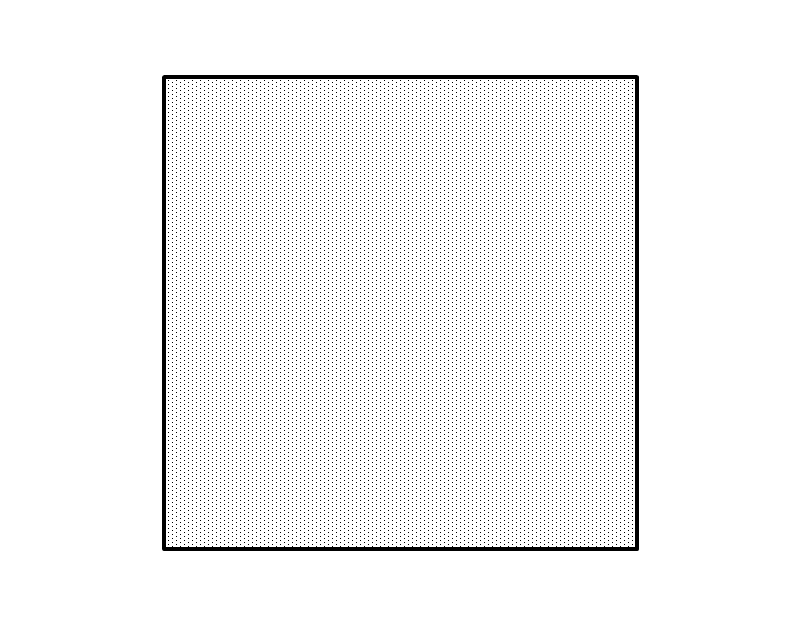
\includegraphics[scale=0.5]{szeliski_naiveEntree.png}}
		\subfigure[Spectrum of the final image : aliasing]{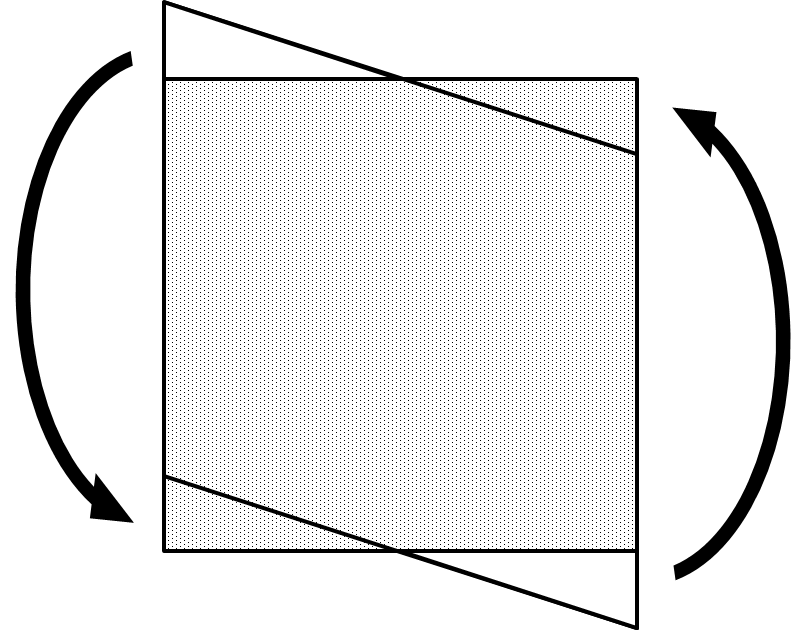
\includegraphics[scale=0.5]{szeliski_naiveSortie.png}}
		\caption{Spectrum of a naive resampling by a shear (cf. partie \ref{label_des_deux_prems_fig_de_szeli})}
		\label{szeliski_decompoNaive}
	\end{figure}
		
	\begin{figure}
		\centering
		\subfigure[Spectrum of the initial image]{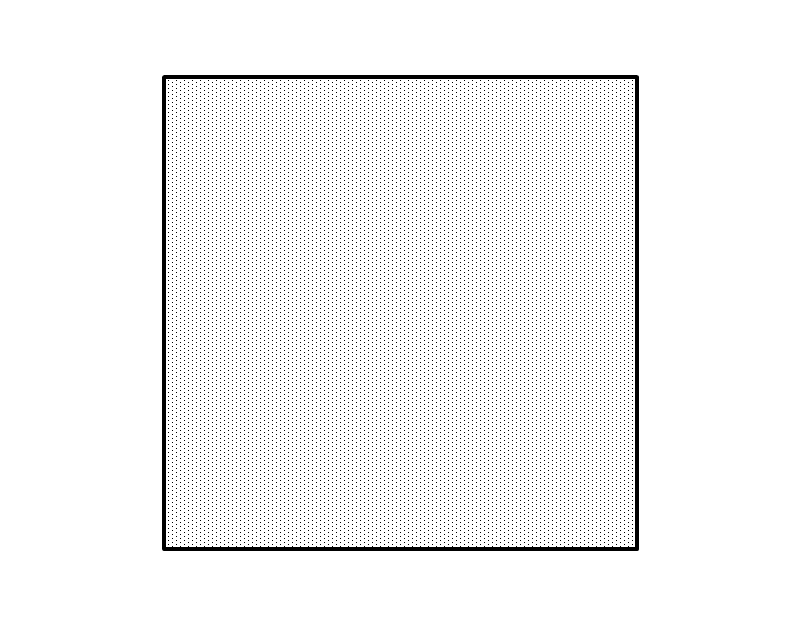
\includegraphics[scale=0.5]{szeliski_szeliskiEntree.png}}
		\subfigure[Spectrum of the image after upsampling]{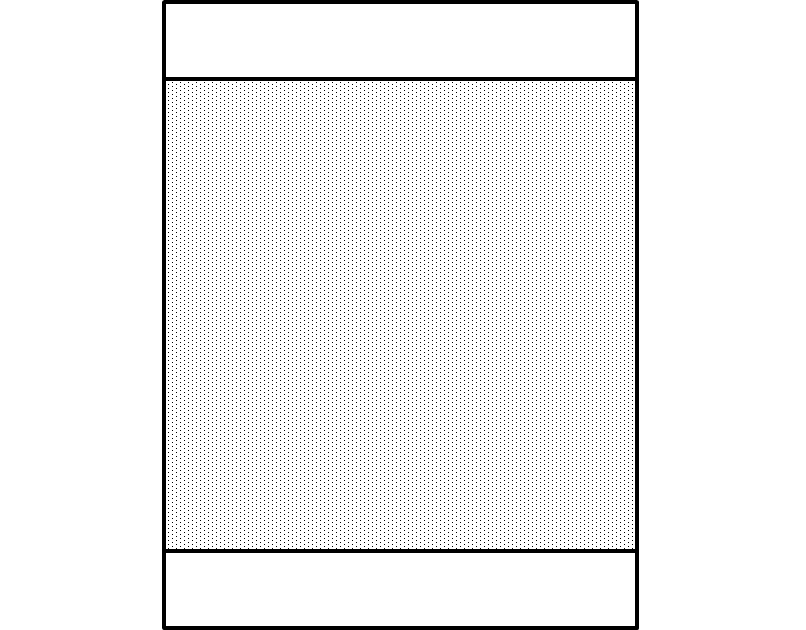
\includegraphics[scale=0.5]{szeliski_szeliskiSurechantillonnage.png}}
		\subfigure[Spectrum of the image after an upsampling and a shear]{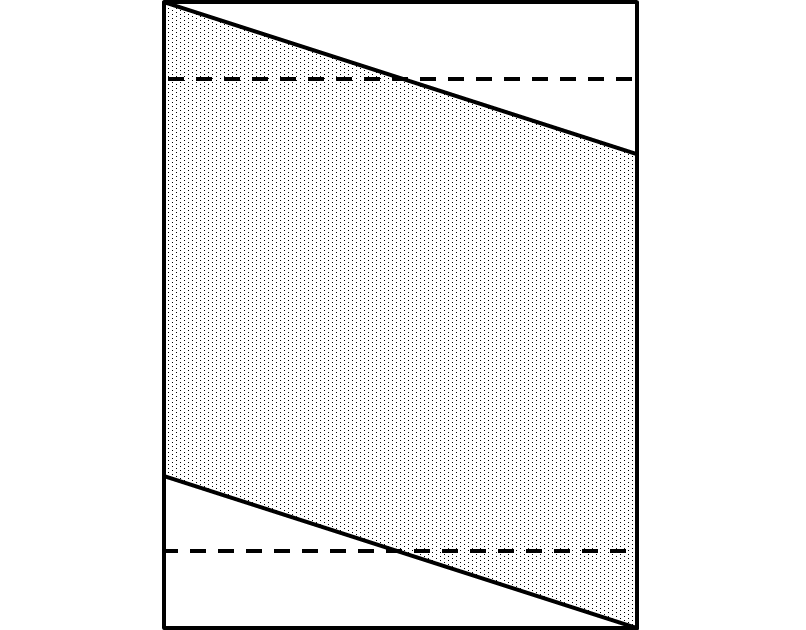
\includegraphics[scale=0.5]{szeliski_szeliskiShear.png}}
		\subfigure[Spectrum of the final image (after an upsampling, a shear and a downsampling, coupled with a low-pass filter)]{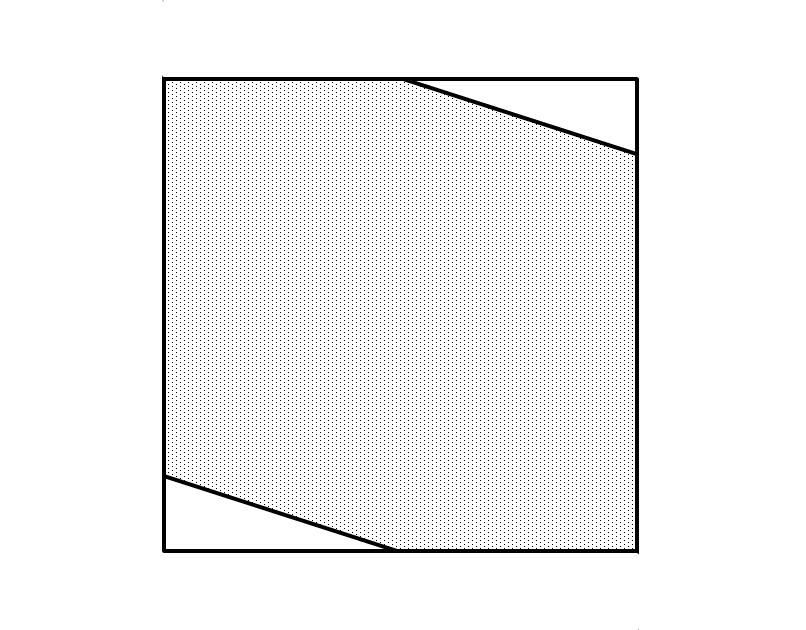
\includegraphics[scale=0.5]{szeliski_szeliskiSortie.png}}
		\caption{Spectrum of an image, resampled by a shear with the multi-pass resampling method (cf. section \ref{label_des_deux_prems_fig_de_szeli}). See the experiment of figure \ref{experiments_decompoSzeliski_sinc} }
		\label{szeliski_decompoSzeliski}
	\end{figure}
	
	%Ces trois opérations sont toutes des \emph{shears} (éventuellement réduits à une dilatation) et seront nommées $\mathcal R$ ; selon qu'elles modifient l'image verticalement (en laissant l'abscisse inchangée) ou horizontalement (en laissant l'ordonnée inchangée), on parlera de $\mathcal R_v$ ou de $\mathcal R_h$ . Ces opérations $\mathcal R$ sont réalisées par une convolution par un noyau d'interpolation, en l'occurrence une fonction de type \emph{raised cosine-weighted sinc}, pour pouvoir atténuer, voire supprimer, les fréquences au-delà d'un certain seuil.
	
\noindent 	Those three operations are all shears (eventually reduced to a dilation) and will be called $\mathcal R$ ; depending on what direction they modify (vertically or horizontally), they will be denoted by $\mathcal R_v$ or $\mathcal R_h$. Each operation $\mathcal R$ is performed by convolving the image by an interpolation kernel, namely a raised cosine-weighted sinc, to attenuate or delete frequences beyond a threshold.
	
	\begin{equation}
	h : x \mapsto \sinc(\frac{x}{T})\frac{\cos(\frac{\pi\beta x}{T})}{1-\frac{4\beta^2x^2}{T^2}}
	\label{szeliski_definition_raisedCosineWeightedSinc}
	\end{equation}
	Here, the period $T$ is equal to one (the pixel size).
	The parameter $\beta$, called roll-off factor, is a crucial choice. If $\beta$ is around $0.36$ (which is the parameter used for most experiments in appendix), the support of $h$ can be reasonably approximated as contained in $[-4,4]$. In that way, the convolution reduces to a sum of nine terms (figure \ref{szeliski_plotRaisedCosine}), as long as the support is not modified.
	
	
%	Le paramètre $\beta$, intitulé \emph{roll-off factor}, peut varier. En prenant $\beta$ autour de $0.36$ (paramètre utilisé pour la plupart des expériences en annexe), on peut considérer que le support de $h$ est compris dans $[-4,4]$, et donc réduire la convolution à une somme d'au plus neuf termes (figure \ref{szeliski_plotRaisedCosine}), tant que le support du filtre n'est pas modifié.
	\label{label_figure_dom_reel_fourier_jt}
	\begin{figure}
		\centering
		\subfigure[Space domain]{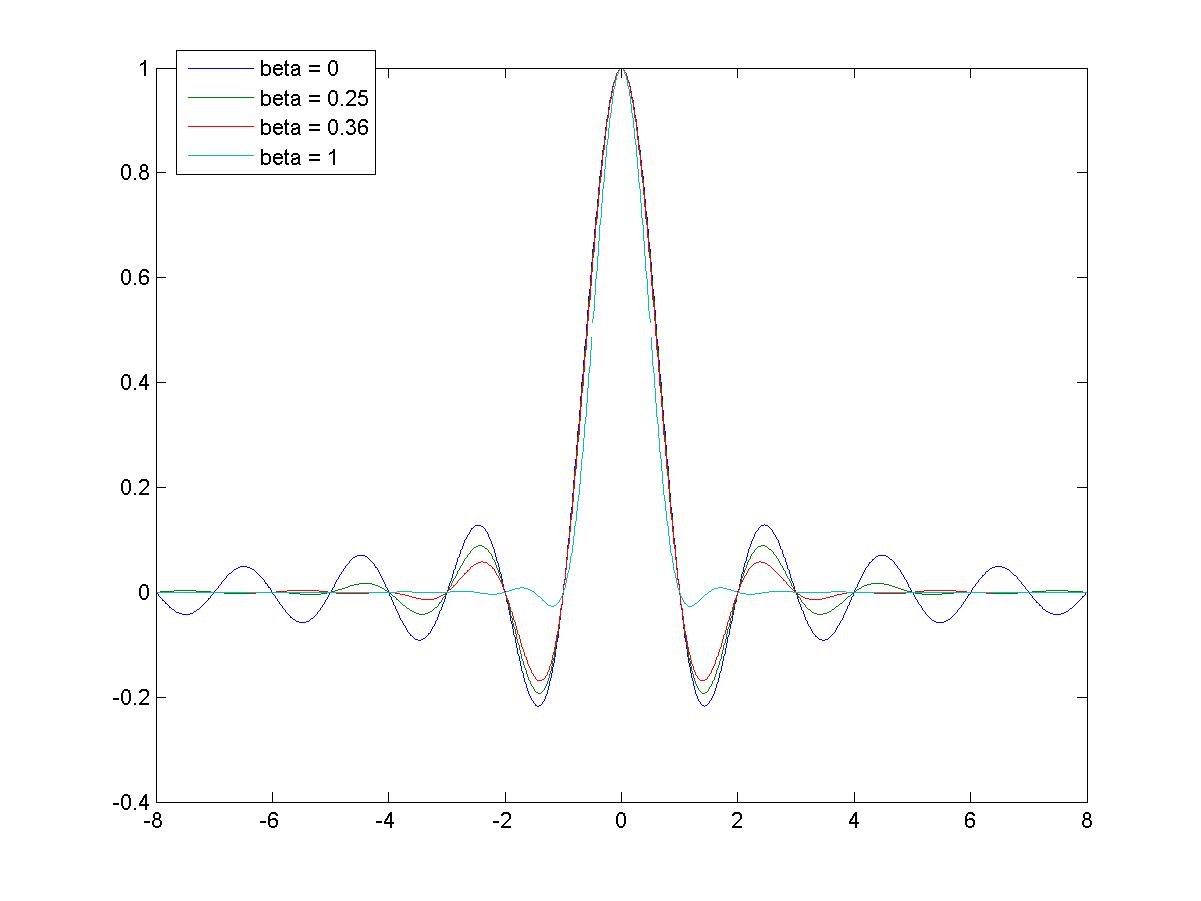
\includegraphics[scale=0.3]{raisedCosine-weightedSinc.jpg}}
		\subfigure[Frequency domain]{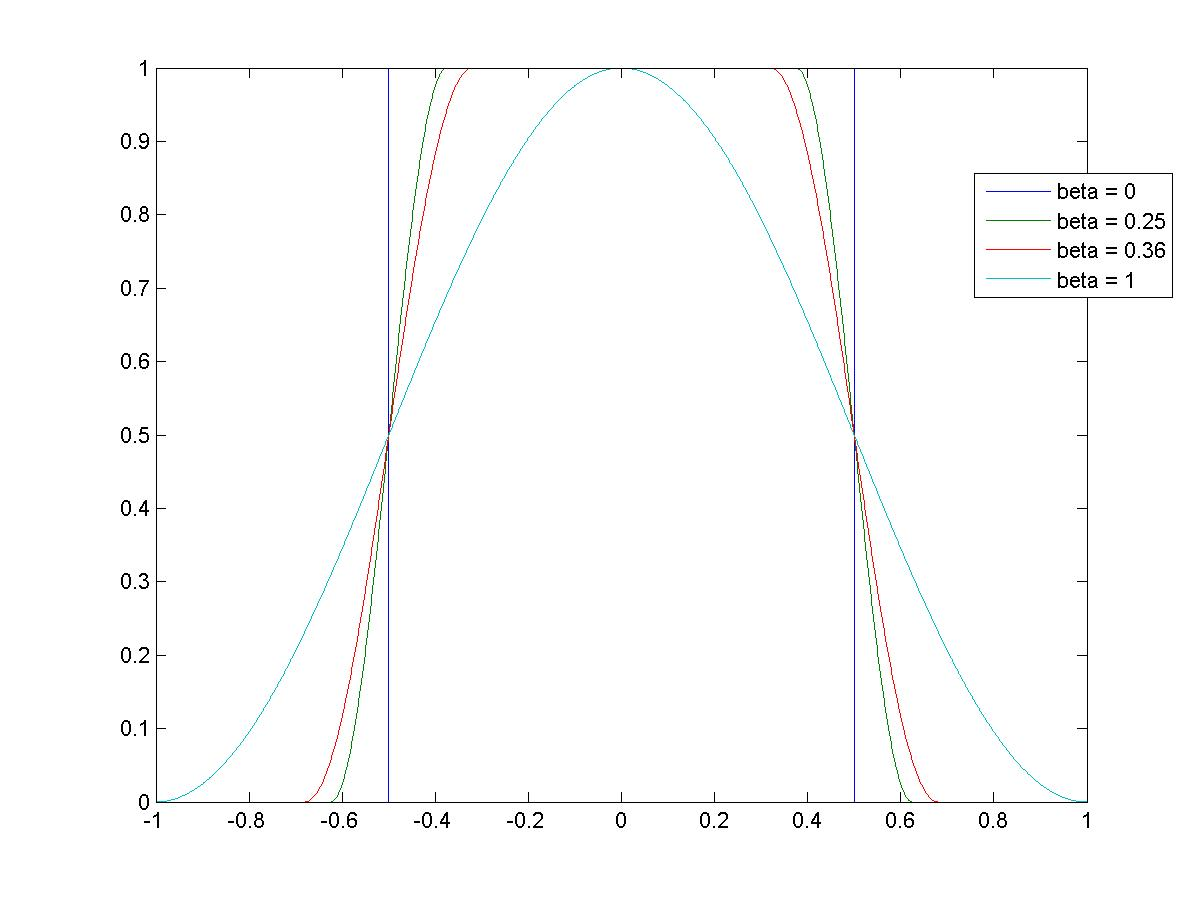
\includegraphics[scale=0.3]{raisedCosine-weightedSinc_spectrum.jpg}}
		\caption{Representations of the \emph{raised cosine-weighted sinc} filter for various values of the parameter $\beta$ (cf. section \ref{label_figure_dom_reel_fourier_jt})}
		\label{szeliski_plotRaisedCosine}
	\end{figure}
	
\noindent	In practice, the support of the filter may vary, depending on the zoom factor $s$, hence the formula to convolve with $h$ (here horizontally) is 
	\begin{equation}
	img_f[i][j] = \displaystyle{\sum_k}h\left(\frac{a_0i+a_1j+t-k}{s}\right)img[k][j]
	\label{formule_convolution_discrete}
	\end{equation}
	where $img_f$ is the output image and $img$ the input image.
	
	
%	En pratique, le support du filtre est adaptatif, et dépend d'un facteur de zoom $s$, d'où la formule de convolution par $h$ (ici convolution selon les abscisses) :
%	où $img_f$ est l'image finale et $img$ l'image initiale.
	
	
\noindent	Multiplying by $s$ the size of support of the filter function (by calling $h(\frac{x}{s})$ instead of $h(x)$, with $s\geq 1$) divides by $s$ the bandwidth of this filter. This protects against aliasing during downsamplings. The coefficient $s$ also depends on the maximal preserved frequencies $u_{max}$ and $v_{max}$ which will be defined in definition \ref{szeliski_def_maximal_preserved_frequencies}.
	
%	En multipliant par $s$ la taille du support du filtre (en appelant $h(\frac{x}{s})$ au lieu de $h(x)$, avec $s\geq 1$), on divise par $s$ la largeur de la bande passante de ce filtre. Cela permet, lors d'un sur-échantillonnage, d'avoir une protection contre l'\emph{aliasing}. Le coefficient $s$ dépend aussi des \emph{fréquences conservées maximales} $u_{max}$ et $v_{max}$ qui seront définies et expliquées plus loin.
	
	The algorithms \ref{szeliski_rh} and \ref{szeliski_rv} dealing with the $\mathcal R_h$ and $\mathcal R_v$ operations are obtained by applying \eqref{formule_convolution_discrete} for every $i$ and $j$ in the output image. \label{szeliski_rv_rh_section}
	
%	En appliquant la formule précédente pour toutes les valeurs de $i$ et $j$ de l'image d'arrivée, on obtient les algorithmes \ref{szeliski_rh} et \ref{szeliski_rv} traitant les opérations $\mathcal R_h$ et $\mathcal R_v$. \label{szeliski_rv_rh_section}
	
	\noindent It is possible in that way to compute $\mathcal R$ and therefore any shear  in three steps and without aliasing. Since any affine map can be decomposed in two shears (proposition \ref{propositionDecompositionAffinite}), any affine map can be processed without aliasing (algorithm \ref{szeliski_affine}).
	
%	On est ainsi capable d'effectuer, en trois étapes $\mathcal R$ et sans \emph{aliasing}, tous les \emph{shears}. Or une affinité se décompose toujours en deux \emph{shears} (proposition \ref{propositionDecompositionAffinite}), on peut donc toujours traiter une affinité quelconque, et ce, sans \emph{aliasing} (algorithme \ref{szeliski_affine}).

	\begin{prop}
	For a fixed image size, the multi-pass resampling method \cite{szeliski2010high} prevents aliasing while preserving as much of the spectrum as possible. %SHMUEL RELIT STP, je ne savais pas traduire
%	Le méthode multi-étapes \cite{szeliski2010high} empêche le repliement du spectre tout en conservant le maximum du spectre.
	\end{prop}
	\begin{proof}
	The effect of the different steps on the spectrum is presented in figure \ref{szeliski_decompoSzeliski} and experimentally verified in figure \ref{experiments_decompoSzeliski_sinc}.
	
\noindent	The downsampling is processed without aliasing by expanding the support of the filter $h$.
	\end{proof}
	
	%\begin{proof}
%	L'effet des différentes étapes sur le spectre est présenté en figure \ref{szeliski_decompoSzeliski} et vérifié en pratique figure \ref{experiments_decompoSzeliski_sinc}.
	
%	Le sous-échantillonnage est effectué sans repliement grâce à un élargissement du support du filtre $h$ (support adaptatif).
	%\end{proof}


	\emph{A priori} this method decomposes any affine map into six steps of type $\mathcal R$ (three per shear). In fact it is possible to merge some of these steps $\mathcal R$ if they act in the same direction. The decomposition can then be reduced to four steps $\mathcal R$ : a vertical up-sampling, a horizontal shear, a vertical shear and finally a horizontal downsampling.
	
%	Cette méthode semble donc décomposer une affinité en six opérations $\mathcal R$ (trois pour chacun des deux \emph{shears}) ; en pratique, il est possible de réunir certains $\mathcal R$, s'ils sont dans la même direction. La décomposition peut alors se réduire à quatre opérations $\mathcal R$ : un sur-échantillonnage vertical, un \emph{shear} horizontal, un \emph{shear} vertical puis enfin un sous-échantillonnage horizontal.
	
\subsection{Steps of the algorithm}
	\label{szeliski_affine_section}
	
	The details of the multi-pass resampling algorithm for an affine map are described in this section. The corresponding algorithms can be found in appendix (algorithms \ref{szeliski_affine} and following).
	
	Let $A$ be the matrix of the inverse affine map of the one supposed to be processed. Let us denote

\[A = \pmatrice{a_{00} & a_{01} & t_0\\ a_{10} & a_{11} & t_1}\]

%	On détaille donc ici les étapes de l'algorithme de traitement d'une affinité par cette méthode multi-étape. Le pseudo-code correspondant est présent en annexe (algorithmes \ref{szeliski_rh}, \ref{szeliski_rv} et \ref{szeliski_affine}).
	
%	On suppose avoir reçu en entrée une image à modifier et la matrice $A$ correspondant à l'affinité inverse de celle à effectuer : l'antécédent du point $(i,j)$ de l'image de sortie se situe donc en $A(i,j)$ sur l'image d'entrée.
	
%	On notera
	
	\subsubsection{A useful transposition}
		\label{szeliski_transpoOpt_section}
		
		The shear is at risk of compressing the image on a few pixels and then expanding it (e.g. when $A$ is a rotation of angle $\frac{\pi}{2}$), this is called the \emph{bottleneck problem} \cite{wolberg1990digital}. To prevent this problem, the image and the matrix can be transposed. Setting
		
%	Les $\mathcal R$ peuvent, si l'affinité est par exemple une rotation d'angle $\frac{\pi}{2}$, compresser l'image sur peu de pixels puis tenter de la dilater ; cet effet est un \emph{bottleneck problem} déjà connu \cite{wolberg1990digital}.
		
	%	On effectue donc éventuellement une transposition (de l'image et de la matrice) pour éviter cet effet : en notant
		\[\hat a_{00} = \frac{a_{00}}{\sqrt{a_{00}^2+a_{11}^2}},\]
		\[\hat a_{01} = \frac{a_{01}}{\sqrt{a_{00}^2+a_{11}^2}},\]
		\[\hat a_{10} = \frac{a_{10}}{\sqrt{a_{10}^2+a_{11}^2}},\]
		\[\hat a_{11} = \frac{a_{11}}{\sqrt{a_{10}^2+a_{11}^2}},\]
		%on transpose dans le cas où $|\hat a_{00}|+|\hat a_{11}|<|\hat a_{01}|+|\hat a_{10}|$.
		the transposition should be applied when $|\hat a_{00}|+|\hat a_{11}|<|\hat a_{01}|+|\hat a_{10}|$.
		This procedure is detailed in algorithm \ref{szeliski_transpoOpt}.
		%Cette transposition correspond à l'algorithme \ref{szeliski_transpoOpt}.
		
	\subsubsection{Decomposition of $A$}
		\label{szeliski_decompositionDeA_section}
		\label{szeliski_frequencesMax_section}
		
		\begin{Def}
		\label{szeliski_def_maximal_preserved_frequencies}
		The maximal preserved frequencies $u_{max}$ and $v_{max}$ are the horizontal and vertical frequencies beyond which the spectrum will be erased by the application of $A$.
		
		They are defined in the frequency domain by figure \ref{uMax_vMax} ; in this definition, the spectrum has been normalized on the square $[-1,1]^2$. Thus, $(u_{max},v_{max})\in [0,1]^2$.
		\end{Def}
		
		Frequencies beyond the maximal preserved frequencies can be filtered out without altering the output spectrum. 
		
%		On introduit les fréquences conservées maximales $u_{max}$, $v_{max}$ : ce sont les fréquences, horizontales et verticales, au delà desquelles les fréquences seront effacées par l'application de $A$ ; elles sont donc définies dans le domaine de Fourier par la figure \ref{uMax_vMax}. Les fréquences au-delà de $u_{max}$ horizontalement et de $v_{max}$ verticalement peuvent donc être filtrées, cela ne changera pas le spectre de sortie. Ces définitions se font après après avoir ramené le spectre sur le carré $[-1,1]^2$.
		
		\begin{figure}
		\centering
		\subfigure[Spectrum of the input image]{
\includegraphics[scale=0.5]{uMax_vMax_spectreEntree.png}}
		\subfigure[Spectrum of the output image]{
\includegraphics[scale=0.5]{uMax_vMax_spectreSortie.png}}
		\subfigure[Spectrum of the input image]{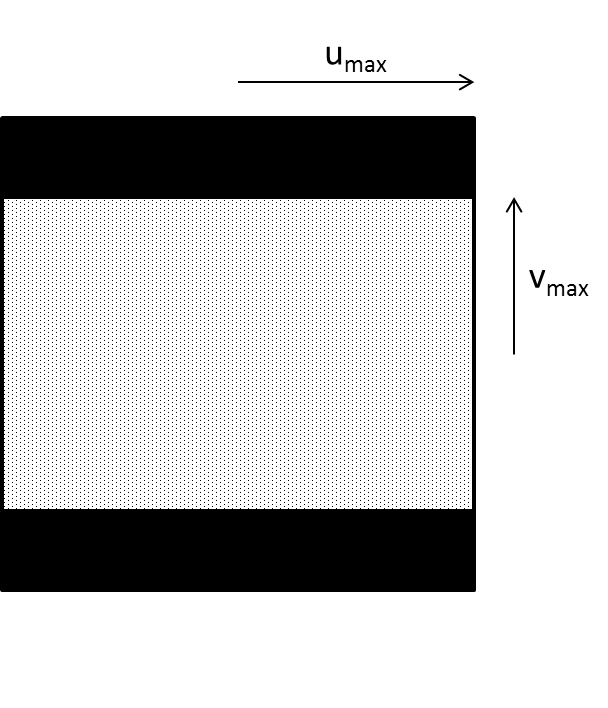
\includegraphics[scale=0.5]{uMax_vMax_spectreUtile.png}}
		\caption{Maximal preserved frequencies (definition \ref{szeliski_def_maximal_preserved_frequencies}). The black areas correspond to the frequencies erased by the application of the affine map}
		\label{uMax_vMax}
		\end{figure}
		
 
		 The frequencies $u_{max}$ and $v_{max}$ can be computed by finding the intersection of the input spectrum (that is to say the square $[-1,1]^2$) with the inverse image of the square by $^t\!A$ Indeed applying $^t\!A$ in the frequency domain is equivalent to applying $A^{-1}$ in the spatial domain. As before $A$ is the inverse of the map applied to the input image. The algorithms \ref{szeliski_intersectionsVerticales} and \ref{szeliski_intersectionsHorizontales} compute the intersection of a segment (which bounds are $(U_1,V_1)$ and $(U_2,V_2)$) with one of the sides of the square $[-1,1]^2$. Both algorithms are used in algorithm \ref{pseudo-code_umax_vmax} to compute $u_{max}$ and $v_{max}$.


		%En pratique, $u_{max}$ et $v_{max}$ s'obtiennent en intersectant le spectre d'entrée (le carré $[-1,1]^2$) et l'image réciproque du carré $[-1,1]^2$ par $^t\!A$ (qui correspond à l'opération dans Fourier ; comme précédemment $A$ désigne l'inverse de l'affinité qu'on applique à l'image). Les algorithmes \ref{szeliski_intersectionsVerticales} et \ref{szeliski_intersectionsHorizontales} réalisent l'intersection d'un segment (d'extrémités $(U_1,V_1)$ et $(U_2,V_2)$) et d'un côté du carré $[-1,1]^2$. L'algorithme \ref{pseudo-code_umax_vmax} s'appuie sur ces algorithmes pour calculer $u_{max}$ et $v_{max}$.
		
		From $A$'s coefficients and the values of $u_{max}$ and $v_{max}$, the coefficients of the vertical upsampling and the horizontal one can be deduced \cite{szeliski2010high} as follows,
		\[r_v \geq \max (1,|a_{01}|u_{max}+\min (1,|a_{11}|v_{max})),\]
		\[r_h \geq \max (1,|a_{10}/a_{11}|r_vv_{max}+\min (1,|b_0|u_{max})).\]

		%À partir des coefficients de $A$ et des valeurs de $u_{max}$ et $v_{max}$, on peut en déduire les coefficients de sur-échantillonnage verticaux et horizontaux nécessaires \cite{szeliski2010high} :
		%\[r_v \geq \max (1,|a_{01}|u_{max}+\min (1,|a_{11}|v_{max}))\]
		%\[r_h \geq \max (1,|a_{10}/a_{11}|r_vv_{max}+\min (1,|b_0|u_{max}))\]

\noindent		By geometric considerations, one can always reduces the upsamplings to $r_h \leq 3$ and $r_v \leq 3$. Indeed, in both unidirectional mappings (those splitted into three $\mathcal R$), $r_h$ and $r_v$ can be reduced to three, thanks to the filtering which attenuates the frequencies beyond $u_{max}$ and $v_{max}$ respectively. Figure \ref{rvleq3} presents this geometric reasoning applied to a mapping on columns (which corresponds to a mapping on rows in the frequency domain).

		%Pour des raisons géométriques, on peut toujours réduire les sur-échantillonnages à $r_h \leq 3$ et $r_v \leq 3$. En effet, pour chacune des deux opérations unidirectionnelles (celles qui seront décomposées en trois $\mathcal R$), le $r_h$ (respectivement $r_v$) peut être réduit à 3, grâce au filtrage qui atténue les fréquences au delà de $u_{max}$ (respectivement $v_{max}$). La figure \ref{rvleq3} présente ce raisonnement géométrique pour une opération sur les colonnes (qui se traduit par une opération sur les lignes dans le domaine de Fourier).
		
		\begin{figure}
		\centering
		\subfigure[$r_v$ not bounded]{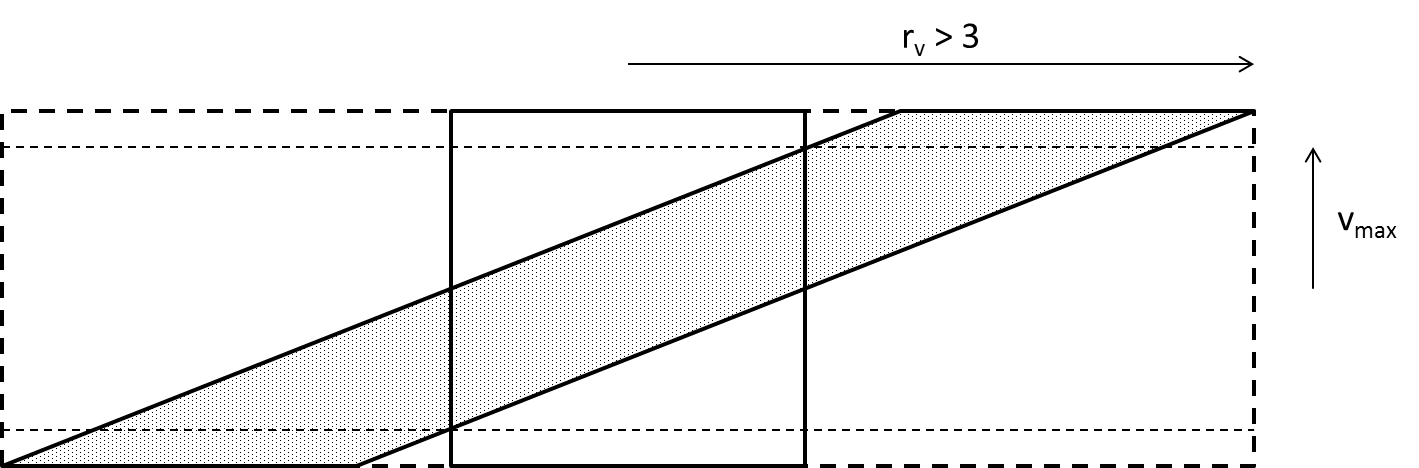
\includegraphics[width=120mm]{rvleq3_notrvleq3.png}}
		\subfigure[$r_v$ bounded by 3 ; the fact the horizontal spacings are unchanged has been used]{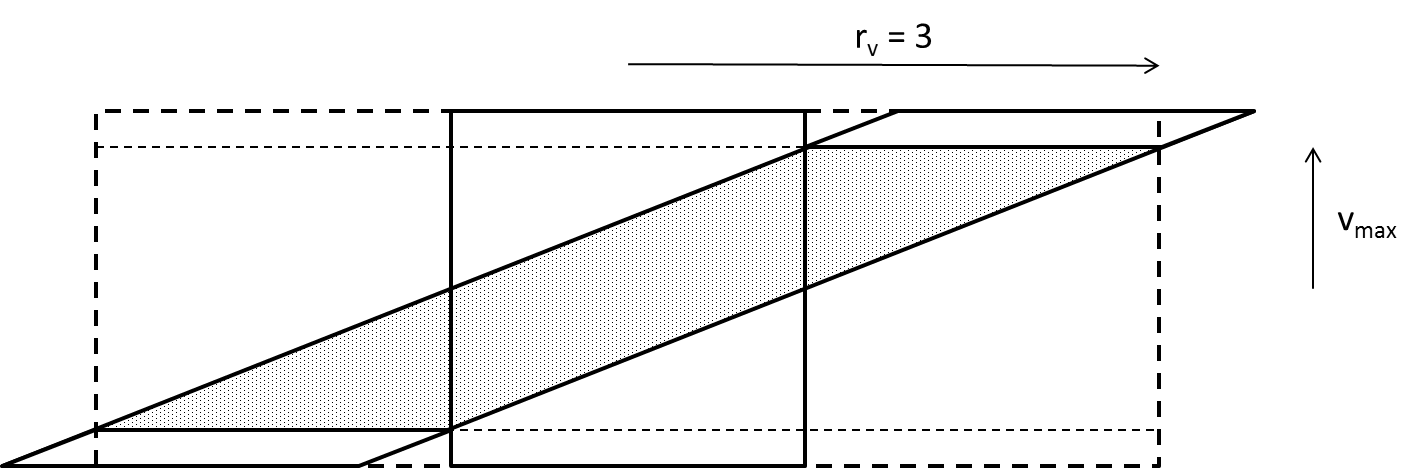
\includegraphics[width=120mm]{rvleq3_rveq3.png}}
		\caption{Reduction of $r_v$ down to $r_v \leq 3$. Beyond $v_{max}$, the frequencies are filtered out. We done by $s$ the parameter of the filter which reduces the bandwidth. Then the value of $r_v$ required to avoid aliasing can be reduced. We can take for $r_v$ the ratio of the length of the dotted rectangle (which is the spectrum after the upsampling) to that of the square (which is the initial spectrum)}
		\label{rvleq3}
		\end{figure}


		\begin{prop}
		\label{propositionDecompositionAffinite}
		Let $A$ be an affine transform given by its projective form, $A = \pmatrice{a_{00} & a_{01} & t_0\\ a_{10} & a_{11} & t_1\\ 0&0&1}$. Then $A$ can be decomposed as follows,
		%Soit $A$ une affinité donnée sous forme projective : $A = \pmatrice{a_{00} & a_{01} & t_0\\ a_{10} & a_{11} & t_1\\ 0&0&1}$.
		%$A$ se décompose de la manière suivante :
		\[
			A = 
			\pmatrice{1 & 0 & 0\\ 0 & \frac{a_{11}}{r_v} & 0\\ 0 & 0 & 1}
			\pmatrice{\frac{b_{0}}{r_h} & \frac{a_{01}}{r_v} & t_2\\ 0 & 1 & 0\\ 0 & 0 & 1}
			\pmatrice{1 & 0 & 0\\ \frac{a_{10}r_v}{a_{11}r_h} & r_v & \frac{t_1r_v}{a_{11}}\\ 0 & 0 & 1}
			\pmatrice{r_h & 0 & 0\\ 0 & 1 & 0\\ 0 & 0 & 1}
		\]
where $b_0 = a_{00} - \frac{a_{01}a_{10}}{a_{11}}$ and $t_2 = t_0 - \frac{a_{01}t_1}{a_{11}}$.
\end{prop}
	\subsubsection{The $\mathcal R$ mappings}
	%\subsubsection{Applications des $\mathcal R$}
		
		All that remains is to to describe the implementation of the four $\mathcal R$ mapping. For each one, the first step is to keep in memory all the values of $h(\frac{k+\varphi}{s})$ where $h$ is the  apodized sinc function defined by \eqref{szeliski_definition_raisedCosineWeightedSinc} and

		%Il ne reste qu'à appliquer les quatre opérations $\mathcal R$.
		%Pour chacune, on commence par stocker les différentes valeurs de $h(\frac{k+\varphi}{s})$ où :
		
\begin{itemize}
		\item $\varphi \in  \left\lbrace\frac{l}{2^b}, l \in \llbracket 0,2^b-1\rrbracket \right\rbrace$ with $b$ the number of precision bits needed.
		\item $k$ is an integer such that $\frac{k}{s}$ is in the support of $h$ ($h(x)$ being nearly zero if $|x|$ is large enough, one assumes that $h$ is compactly supported).
		\end{itemize}
		Thus all the values of $h$ used for the convolution can be easily found.



%\begin{itemize}
%		\item $\varphi$ parcourt $2^b$ nombres rationnels de $[0,1]$ avec $b$ le nombre de bit de précision voulu
%		\item $k$ parcourt les entiers tels que $\frac{k}{s}$ soit dans le support de $h$ ($h(x)$ étant presque nul quand $|x|$ est assez grand, on suppose %$h$ à support compact)
%		\end{itemize}
%		On a ainsi accès rapidement à toutes les valeurs de $h$ qui peuvent être nécessaires à la convolution.
%shmuel
	\section{Irregular sampling for a homography}
		\label{decomp_geo_hom}
		\subsection{Geometric decomposition}
			\label{DecompositionGeometrique}
			The new method for homography resampling is based on the decomposition of a homography interpreted as a result on an image of a motion in space of the camera. The section below presents that decomposition (theorem \ref{thepropdecomp} and corollary \ref{thecorollairedecomp}).


%La nouvelle méthode de traitement des homographies repose sur la décomposition d'une homographie qui permet d'interpréter cette dernière en terme de mouvement de caméra. La partie ci-dessous présente cette décomposition.

\ssse{Modeling camera motion}
%\ssse{Modélisation de mouvement de caméra}
\label{mouv_de_camera}

In this section we define the geometric model of a pinhole camera, and show that when its application is restricted to a plane, it can be interpreted as a planar homography. Conversely we shall see that any planar homography can be interpreted in that way. In the pinhole model, the camera is reduced to a projection from the 3D space  onto a plane trough rays passing by a focus $F$,  as illustrated in figure \ref{shmdecomp}.

%On étudie ici un cas a priori particulier d'homographie $h$ : les homographies que l'on peut interpréter comme un mouvement de caméra idéale. On montrera par la suite que c'est en fait un cas général.

%Nous modéliserons la situation en supposant que la scène filmée est plane. Cela suppose que l'on filme une surface soit sans aucun relief, soit avec un relief négligeable devant la distance à la caméra, afin qu'il ne soit pas perceptible. La figure \ref{shmdecomp} illustre la modélisation utilisée pour la caméra idéale. La caméra idéale se modélise donc par la projection d'un plan sur un autre en passant par un foyer $F$, en négligeant les lentilles ou les dispositifs correcteurs présents dans les caméras réelles.

\begin{figure}[h!]

\centering
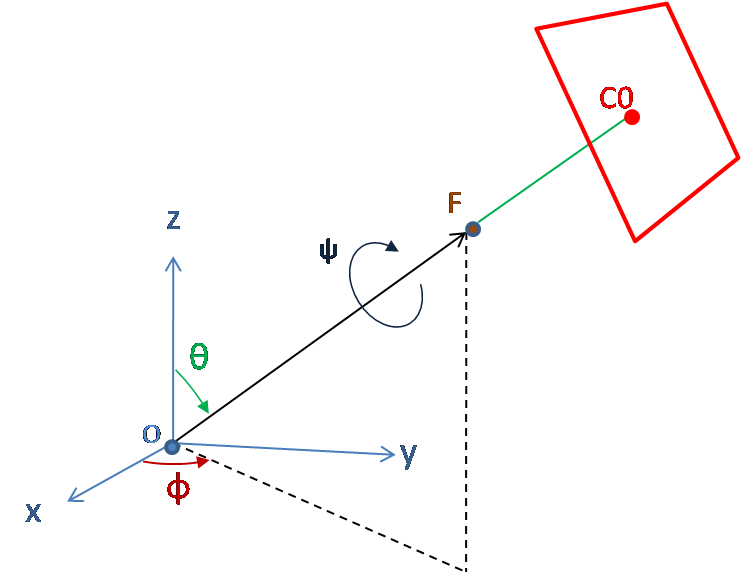
\includegraphics[width=10cm]{shema_decomp.png}
\caption{Parameterization of a pinhole camera taking an image of the $(x,y)$ plane. $F$ is the focus of the camera, the red plane is the image plane of the camera.  One point of the image plane is obtained by the projection of a point of the plane $(x,y)$ through the point $F$. (cf. part \ref{mouv_de_camera})}
\label{shmdecomp}
\end{figure}

We consider the Euclidean space $\mathbb{R}^3$ with origin $O=(0,0,0)$ and its canonical basis denoted by $(\xbf_0,\ybf_0,\zbf_0)$.
%On se place dans l'espace vectoriel $\mathbb{R}^{3}$ on note $O$ l'origine $(0,0,0)$ et $(\xbf_0,\ybf_0,\zbf_0)$ la base canonique.
\begin{itemize}
\item Let $F$ and $C_0$ be two distinct points in $\mathbb{R}^{3}$.
\item Let $\mathcal{P}$ be the affine plane through $C_0$ and of normal vector $\overrightarrow{FC_0}$.
\item Let $\wbf$ be the vector $\frac{\overrightarrow{FC_0}}{|| \overrightarrow{FC_0}||}$
\item Let $\delta$ be the distance $|| \overrightarrow{FC_0}||$
\end{itemize}

\begin{Def}
With the above notation, we call projective mapping  and denote by $H$  the map associating with every point $X$ in $\mathbb{R}^3$ the intersection point of the straight line $(X, F)$ with the plane $\mathcal{P}$. This map has for parameters $F, \wbf$ and $\delta$.
\label{DefProjective}
%L'application projective $H$, est l'application qui à un point $X$ de $\mathbb{R}^{3}$ associe le point d'intersection entre la droite $(XF)$ et le plan $\mathcal{P}$. $H$ dépend du triplet $(F,\wbf,\delta)$.
\end{Def}

\begin{remarque}
$F$ is the focus of the camera and the plane $\mathcal{P}$ is the camera plane, on which the image contained in the plane $(x,y)$ is projected. The optical axis of the camera is the straight line $(FC_0)$ directed by $\wbf$, $\delta$ is the focal distance..
\end{remarque}

We shall denote by $\mathcal{P}'$ be the affine plane of $\mathbb{R}^{3}$ containing $F$ and parallel to the plane $\mathcal{P}$.
\begin{lem}
The projective mapping  $H$ of definition \ref{DefProjective} is defined on $\mathbb{R}^3 \setminus \mathcal{P}'$ and
\begin{equation}
H(X) = C_0 +  \delta \frac{\overrightarrow{XF}-(\overrightarrow{XF}\cdot \wbf )\wbf}{\wbf \cdot \overrightarrow{XF}}. 
\label{formul_lem_app_proj}
\end{equation}
\label{lem_app_proj}
\end{lem}

\begin{figure}[h!]

\centering
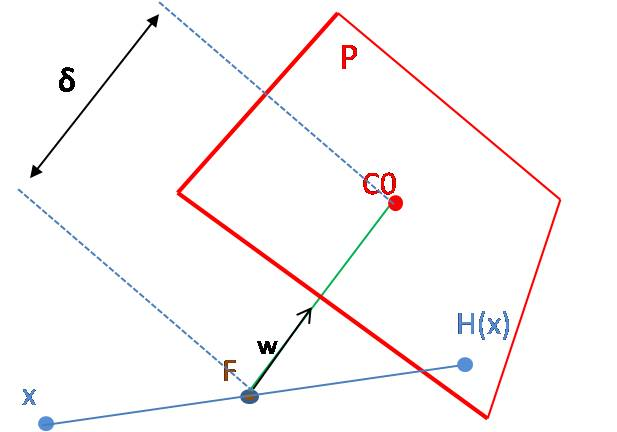
\includegraphics[width=10cm]{schema_lemme_1_bis.jpg}
\caption{Illustration of lemma \ref{lem_app_proj}}
\label{shmlemme1}
\end{figure}

%JEN SUIS LALALALALALLALALALA
\begin{proof}
If $X\in \mathbb{R}^3 \setminus \{F\}$ the straight ligne $(XF)$ and meets $\mathcal{P}$ if and only if it is not parallel to  $\mathcal{P}$ and therefore if and only if $X\in \mathbb{R}^3 \setminus \mathcal{P}'$. In that case, there exists $t_X\in \mathbb{R}$ such that
\begin{equation}
H(X)=X+t_{X}\overrightarrow{XF}.
\end{equation}
So
\begin{equation}
\overrightarrow{FH(X)} = (t_X-1)\overrightarrow{XF}
\label{formule_H}
\end{equation}
As $H(X)\in \mathcal{P}$
\begin{equation*}
\overrightarrow{FH(X)}\cdot \wbf =\delta.
\end{equation*}
Using this and \eqref{formule_H}, we obtain 
\begin{equation*}
t_{X}=1+\frac{\delta}{\wbf \cdot \overrightarrow{XF}},
\end{equation*}
 Then it can be deduced using this and \eqref{formule_H} that
 \begin{equation*}
 \overrightarrow{FH(X)}=\frac{\delta}{\wbf \cdot \overrightarrow{XF}}\overrightarrow{XF},
 \end{equation*}
 so that
 \begin{equation*}
 H(X)=C_0-\overrightarrow{FC_0}+\frac{\delta}{\wbf \cdot \overrightarrow{XF}}\overrightarrow{XF}.
 \end{equation*}
 Since $\overrightarrow{FC_0}=\delta\wbf$, it can be deduced that
\begin{equation*}
H(X) = C_0 +  \delta \frac{\overrightarrow{XF}-(\overrightarrow{XF}\cdot \wbf )\wbf}{\wbf \cdot \overrightarrow{XF}}.
\end{equation*}
\end{proof}


\begin{remarque}
The plane $\mathcal{P}'$ is the blindspot of the camera ; in the case of a real camera, that blindspot should include also the half space "behind" the camera..
\end{remarque}


\begin{Def} 
We shall denote by $P$ the canonical plane $(O,\xbf_0,\ybf_0)$.
We shall call target point the intersection point of the straight line $(FC_0)$ and of the plane $P$. This target point exists if and only if $(FC_0)$ is not parallel to $\mathcal{P}$. When it exists we will denote it by $X_v$ and we have
\begin{equation*}
X_v=F-\wbf \delta',~~~~~~\delta'=\frac{\overrightarrow{OF}\cdot \zbf_0}{\wbf \cdot \zbf_0}.
\label{formule_point_vise}
\end{equation*}
\label{point_vise}
\end{Def}


\begin{remarque}
If the target point does not exist, this means that it is at infinity and that the camera targets the horizon.
\end{remarque}


In all that follows we assume that the camera has its target point in $P$.

\begin{Def}
We call projective planar mapping $H^*$ related to $H$ the restriction of $H$ to $P\setminus (\mathcal{P}'\cap P)$. 
If $\wbf \perp P $, then $H^*$ is defined on $P$. Otherwise $H^*$ is defined on $P\setminus D$ where $D$ is the straight line
\begin{equation*}
D=\left\{ X\in P | \overrightarrow{XF}\cdot \wbf = 0\right\}.
\end{equation*}
\end{Def}

\begin{remarque}
We can interpret the situation as follows: the scene is a fully planar image $P$ photographed by the pinhole camera $H$.  Then, from a point $X\in P$ of the filmed scene, the mapping $H^*$ returns the point in $P_2$ which is its image by the camera. The straight line $D'=\{ X \in \mathcal{P} | \overrightarrow{XF} \cdot \zbf_0 =0 \}$ is called the horizon of $H^*$.
\end{remarque}

From now on we associate with the affine plane $\mathcal{P}$ a direct normalized basis $(C,\ubf,\vbf)$. 

\begin{Def}
 The homography related with $H^*$ in the basis $(C,\ubf,\vbf)$ is the mapping
\begin{equation}
h : (x,y)  \mapsto \left( \overrightarrow{CH^*(X)}\cdot \ubf , \overrightarrow{CH^*(X)}\cdot \vbf \right)
\label{formule_homographie_H}
\end{equation}
with $X=x~\xbf_0 + y~\ybf_0 $.
\label{def_homographie_H}
\end{Def}

Let $D,D'$ be the straight lines in $\mathbb{R}^2$ obtained when $P$ and $\mathcal{P}$ have the basis $(O,\xbf,\ybf)$ and $(C,\ubf,\vbf)$. Then $h:\mathbb{R}^2  \setminus D \mapsto \mathbb{R}^2  \setminus D'$ is a bijective mapping.

%\begin{remarque}
%From a point $X\in P$ of coordinates $(x,y)$, the mapping $h$ returns the coordinates of the point $H^*(X)$ of the numeric image coming from the camera. 
%\end{remarque}

\begin{Def}
\label{decompogeo_def_angles}
Let $(\phi , \theta ,\psi )$ be the three Euler angles defining the orientation of the basis $(\ubf,\vbf,\wbf)$ with respect to the basis $(\xbf_0,\ybf_0,\zbf_0)$ (figure \ref{img_angles}) :
\begin{itemize}
\item $\phi$ is the first rotation around the axis $(X_v ,\zbf_0)$
\item $\theta$ is the second rotation around the axis $(X_v , \ybf_2 )$
\item $\psi$ is the third rotation around the axis $(X_v , \wbf )$
\end{itemize}
\end{Def}

\begin{figure}
\centering
\subfigure[rotation of angle $\phi$]{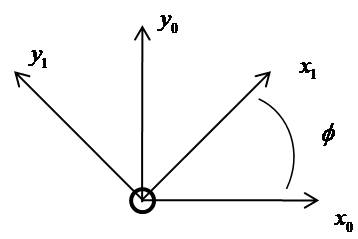
\includegraphics[width=5cm]{graphe1.jpg}}
\subfigure[rotation of angle $\theta$]{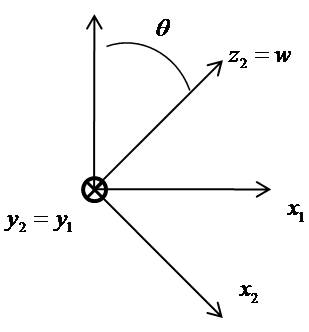
\includegraphics[width=5cm]{graphe2.jpg}}
\subfigure[self rotation (of angle $\psi$)]{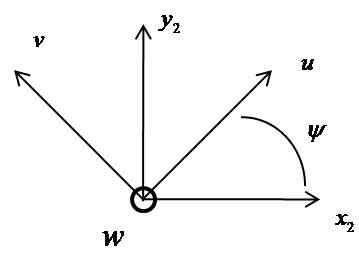
\includegraphics[width=5cm]{graphe3.jpg}}
\caption{Euler angles between the bases $(\ubf,\vbf,\wbf)$ and $(\xbf_0,\ybf_0,\zbf_0)$ (definition \ref{decompogeo_def_angles})}%j'ai vérifié, bases est le pluriel de basis
\label{img_angles}
\label{decompgeo_rotationPropre}
\end{figure}

In what follows we set $\cbf= \left (\overrightarrow{C_0 C}\cdot \ubf , \overrightarrow{C_0 C}\cdot \vbf \right)$ and $\xbf_v=\left( \overrightarrow{O X_v}\cdot \ubf , \overrightarrow{O X_v}\cdot \vbf \right )$.\\

 \begin{Def}
We call unidirectional homography a mapping $h:\mathbb{R}^{2} \ra \mathbb{R}^{2}$ defined by
\begin{equation*}
h(x,y)=\left ( \frac{ax+p}{rx+t} , \frac{cy+p}{rx+t} \right)
\end{equation*}
where $a,p,c,q,r,t$ are reals numbers.
\label{homo_uni_direc}
\end{Def}

\begin{prop}
Let $h$ be a planar homography as specified in Definition \ref{formule_homographie_H}. Then $h$ can be factorized as follows
\begin{equation}
h = \tau_{\cbf}   \circ R_{\psi} \circ z_{\frac{\delta}{\delta'}} \circ h_{\theta,\delta'} \circ R_{\phi} \circ \tau_{\xbf_v},
\label{formul_decomp}
\end{equation}
where $R_\alpha$ denotes the planar rotation of angle $\alpha$, $z_\lambda$ is the zoom of factor $\lambda$, $\tau_\ybf$ is the translation by the vector $-\ybf$ and $h_{\theta,\delta'}$ is the unidirectional homography (see definition \ref{homo_uni_direc}) defined by
\begin{equation}
h_{\theta,\delta'}(x,y)=\left(\frac{-cos(\theta)x}{1-\frac{sin(\theta)}{\delta'}x} ,\frac{-y}{1-\frac{sin(\theta)}{\delta'}x}\right).
\label{mise_perspective}
\end{equation}
\label{prop_decomp}
\end{prop}








\begin{proof}
Using \eqref{formule_homographie_H}, definition \ref{def_homographie_H} and \eqref{formul_lem_app_proj} of lemma \ref{lem_app_proj}, we have
\begin{equation*}
h((x,y))=\left( \delta \frac{\overrightarrow{XF}\cdot \ubf}{\overrightarrow{XF} \cdot \wbf} +\overrightarrow{CC_0 } \cdot \ubf, \delta \frac{\overrightarrow{XF}\cdot \vbf}{\overrightarrow{XF} \cdot  \wbf}+\overrightarrow{CC_0 }\cdot \vbf \right).
\end{equation*}
where $X=x \xbf_0 + y \ybf_0 $. By introducing the target point $X_v$ (see \eqref{formule_point_vise} of definition \ref{point_vise}) and the translation $\tau_c$ we have
\begin{equation}
(\tau_\cbf^{-1} \circ h)((x,y)) = \left ( -\delta \frac{\overrightarrow{X_vX}\cdot \ubf}{\delta' -\overrightarrow{X_vX} \cdot \wbf},-\delta \frac{\overrightarrow{X_vX}\cdot \vbf}{\delta' -\overrightarrow{X_vX} \cdot \wbf} \right).
\label{decomp_formul_intermediaire_1}
\end{equation}

\noindent We define an intermediate basis $(\xbf_1 ,\ybf_1 ,\zbf_1)$  $(\xbf_2 ,\ybf_2 ,\zbf_2)$, in order to decompose the three rotations $\phi,\theta,\psi$ (figures \ref{img_angles} and \ref{decompgeo_rotationPropre} ). Then we have
\begin{equation*}
\ubf=\cos(\psi)\xbf_{2}+\sin(\psi)\ybf_{2} ,  \vbf=-\sin(\psi)\xbf_{2}+\cos(\psi)\ybf_{2} \text{ and } \wbf=\zbf_2.
\end{equation*}

\noindent Denoting by $R_{s}$ the rotation of angle $s$ and using  \eqref{decomp_formul_intermediaire_1}, we obtain
\begin{equation*}
(\tau_{\cbf}^{-1} \circ h)((x,y)) = R_{\psi}\left(\frac{\delta \overrightarrow{X_v X}\cdot \xbf_{2} }{\delta'-\zbf_2 \cdot \overrightarrow{X_v X}},\frac{\delta \overrightarrow{X_v X}\cdot \ybf_{2}}{\delta'-\zbf_2 \cdot \overrightarrow{X_v X}}  \right).
\end{equation*}
Let $i$ be the mapping such that $i(x,y)=x \xbf_0 + y \ybf_0$. Since $i(\xbf_v)=\overrightarrow{O X_v}$ we have
\begin{equation*}
(R_{\psi}^{-1} \circ \tau_{\cbf}^{-1}  \circ h)((x,y))=\delta \left(\frac{-i(\tau_{\xbf_v} ((x,y)))\cdot \xbf_{2} }{\delta'-\zbf_2 \cdot i(\tau_{\xbf_v} ((x,y)))},\frac{-i(\tau_{\xbf_v} ((x,y)))\cdot \ybf_{2}}{\delta'-\zbf_2 \cdot i(\tau_{\xbf_v} ((x,y)))}  \right) 
\end{equation*}
Since $\zbf_{2}=cos(\theta)\zbf_{1}+sin(\theta)\xbf_{1}$, $\xbf_{2}=cos(\theta)\xbf_{1}-sin(\theta)\zbf_{1}$ (figure \ref{img_angles}) and $\zbf_{1}\perp P_{1}$, we have
\begin{equation*}
(R_{\psi}^{-1} \circ \tau_{\cbf}^{-1}  \circ h)((x,y))=\frac{\delta}{\delta'}\left(\frac{-\cos(\theta)i(\tau_{\xbf_v} ((x,y)))\cdot \xbf_{1} }{1-\frac{sin(\theta)}{\delta'}\xbf_{1}\cdot i(\tau_{\xbf_v}((x,y)))}, \frac{-i(\tau_{\xbf_v} ((x,y)))\cdot \ybf_{1}}{1-\frac{sin(\theta)}{\delta'}\xbf_{1}\cdot i(\tau_{\xbf_v}((x,y)))}  \right) 
\end{equation*}
Let $h_{\theta,\delta'}$ be defined by
\begin{equation*}
h_{\theta,\delta'}(x',y')=\left(\frac{-\cos(\theta)x'}{1-\frac{\sin(\theta)}{\delta'}x'} ,\frac{-y'}{1-\frac{\sin(\theta)}{\delta'}x'}\right)
\end{equation*}
Then
\begin{equation*}
(R_{\psi}^{-1} \circ \tau_{\cbf}^{-1} \circ h)((x,y))= \frac{\delta}{\delta'}h_{\theta,\delta'}\left ( i(\tau_{\xbf_v}((x,y))) \cdot \xbf_{1}, i(\tau_{\xbf_v}((x,y))) \cdot \ybf_{1}\right).
\end{equation*}
\label{figure_de_rotations_18}
Since $\xbf_{1}=\cos(\phi)\xbf_{0}+\sin(\phi)\ybf_{0}$ et $\ybf_{1}=-\sin(\phi)\xbf_{0}+\cos(\phi)\ybf_{0}$ (figure \ref{img_angles}), we have

\begin{eqnarray*}
(R_{\psi}^{-1} \circ \tau_{\cbf}^{-1} \circ h)((x,y)) &=& \frac{\delta}{\delta'}h_{\theta,\delta'}\left ( R_{\phi}(i(\tau_{\xbf_v}((x,y))) \cdot \xbf_{0}, i(\tau_{\xbf_v}((x,y))) \cdot \ybf_{0})\right)\\
                                               &=&\frac{\delta}{\delta'} (h_{\theta,\delta'}\circ R_{\phi} \circ \tau_{\xbf_v})((x,y)).
\end{eqnarray*}
Denoting zooms $z_{\lambda}:X\rightarrow \lambda X$, the claim is verified since
\begin{equation*}
h = \tau_{\cbf} \circ R_{\psi} \circ z_{\frac{\delta}{\delta'}} \circ h_{\theta,\delta'} \circ R_{\phi} \circ \tau_{\xbf_v}
\end{equation*}
\end{proof}


\begin{remarque}
Resampling an image by the homography $h$ simulates a change of the point of view on the input image. This change of viewpoint has parameters $(\phi,\theta,\psi,\delta,\delta',\xbf_v,\cbf_v)$, which are not independent. %The case in which the camera is targeting the horizon has not been discussed, translations $\tau_\cbf$ allow to avoid this.
\end{remarque}

\begin{remarque}
The previous method does not model every affine transform. Indeed the function $h$ defined by 
\begin{equation*}
h = \tau_{\cbf}   \circ R_{\psi} \circ z_{\frac{\delta}{\delta'}} \circ h_{\theta,\delta'} \circ R_{\phi} \circ \tau_{\xbf_v}
\end{equation*}
is affine if and only if $\theta=0$. In that case we have
\begin{equation*}
h= \tau_{\cbf} \circ z_{-\frac{\delta}{\delta'}} \circ R_{\phi+\psi} \circ \tau_{\xbf_{v}}
=\tau' \circ z_{-\frac{\delta}{\delta'}} \circ  R_{\phi+\psi}.
\end{equation*}
However the affinity can be seen as a limit case. Let $k$ be the ratio $\frac{\delta}{\delta'}$. If $\delta'$ and $\delta$ tend to $+\infty$, the function $h_{\theta,\delta'}$ tends to $h_{\theta,\infty}$ defined by
\begin{equation*}
h_{\theta,\infty}=(x,y)=(-\cos(\theta)x,-y).
\end{equation*}
Physically, this process is equivalent to moving away from the plane while increasing the focal distance in order to keep the size of the output image constant.

\noindent If $h_\infty = z_{-\frac{\delta}{\delta'}} \circ \tau_{\xbf} \circ R_{\phi} \circ h_{\theta,\infty} \circ R_{\psi} \circ \tau_{\xbf_{v}}$, the linear part of $h_{\infty}$ can be represented by a matrix $2\times2$

\begin{equation*}
R_{\psi} \cdot 
\begin{pmatrix}
-k\cos(\theta)&0\\
0&-k
\end{pmatrix}
\cdot R_{\phi}
\end{equation*}

\begin{lem}
Let $M$ be an invertible $2\times 2$ matrix. Then (by the singular value decomposition \cite{morel2009asift}) there exist two rotation matrix $R_1$ and $R_2$ and a diagonal matrix $D$ such that $M = R_1 \cdot D \cdot R_2$.
\label{decomp_valeur_sing}
\end{lem}

\noindent Using lemma \ref{decomp_valeur_sing}, it can be deduced that for every bijective affinity $A$, there exists a camera movement $h$ such that $h_\infty = A$. Moreover it can be assumed that $h$ has no output translation.
\end{remarque}

\subsubsection{Application of the decomposition to homographies}
The previous results show that all homographies can be decomposed as described in the next theorem.

%Le résultat précédent montre que certaine homographie peuvent se décomposer de la
\begin{thm}
Let $h$ be a planar homography. If $h$ is not an affine map, then there exist parameters $(\phi,\theta,\psi,\delta,\delta',(x_1,y_1),(x_2,y_2))$ such that
\begin{equation*}
h = \tau_{(x_2,y_2)} \circ R_{\psi} \circ z_{\frac{\delta}{\delta'}} \circ h_{\theta,\delta'} \circ R_{\phi} \circ \tau_{(-x_1,-y_1)}
\end{equation*}
This decomposition is not unique. More precisely, for all $\lambda \in ]0,1[$,

  \begin{equation*}
h = \tau_{(x_2,y_2)} \circ z_{\frac{\delta}{\delta'}}  \circ R_{\psi} \circ h_{\theta,\delta'} \circ R_{\phi} \circ \tau_{(-x_1,-y_1)}
  \end{equation*}
  where 
 \begin{equation*}
x_2=\frac{ar+sb+\hat r \lambda}{r^2 +s^2}, y_2=\frac{cr+sd+\hat s \lambda}{r^2 +s^2}, (x_1 , y_1) = h^{-1}(x_{2},y_{2})
  \end{equation*}
 \begin{equation*}
 \cos( \phi )= - \frac{r}{\sqrt{r^2 + s^2}}, \sin( \phi )= - \frac{s}{\sqrt{r^2 + s^2}},\cos( \psi ) =- \frac{\hat r}{\sqrt{\hat r^2 + \hat s^2}}, \sin( \psi ) = \frac{\hat s}{\sqrt{\hat r^2 + \hat s^2}}
 \end{equation*}
 \begin{equation*}
 \frac{\delta}{\delta'}=|\lambda|\left(\frac{\hat r^2 + \hat s^2}{r^2 + s^2}\right)^{3/2}, \cos(\theta)=\lambda, \sin(\theta)=\sqrt{1-\lambda^2}, \delta'=  \frac{\sqrt{(r^2 + s^2)(1-\lambda^2)}}{|\lambda| (\hat r^2+\hat s^2)}
 \end{equation*}
\label{thepropdecomp}
\end{thm}

\begin{corollaire} If $h$ is a planar homography and $h$ is not affine, then there exists a translation $\tau$, two rotations $R_\phi ,R_\psi$ and a unidirectional homography $\tilde{h}$ such that
\begin{equation}
h=\tau \circ R_\psi \circ \tilde{h} \circ R_\phi,
\label{formule_decomposition_effective}
\end{equation}
yet this decomposition is not unique.
\label{thecorollairedecomp}
\end{corollaire}

\begin{remarque}
The formula \eqref{formule_decomposition_effective} is the main ingredient of algorithm \ref{pseudoCodeDecompo}.
\end{remarque}


\begin{proof}
	 Using theorem \ref{thepropdecomp}, there exist $(\phi,\theta,\psi,\delta,\delta',\xbf_v,\cbf)$ such that 
	 \begin{equation*}
	 h = \tau_{\cbf} \circ R_{\psi} \circ z_{\frac{\delta}{\delta'}} \circ h_{\theta,\delta'} \circ R_{\phi} \circ \tau_{\xbf_v}.
	 \end{equation*}
	 
\noindent Observe that $R_\psi$ and $z_{\frac{\delta}{\delta'}}$ commute. Let $\tau'$ be the translation such that $\tau' \circ R_\phi =  R_\phi \circ \tau_{\xbf_v}$.\\
	 Then setting $\tilde{h} = z_{\frac{\delta}{\delta'}} \circ h_{\theta,\delta'} \circ \tau'$ it can be easily verified that $\tilde{h}$ is a unidirectional homography.
	 \end{proof}
	\label{ref_schema_decomp_cool}
	\begin{figure}
		\centering
		\subfigure[Input image]{
		\centering
		{
\includegraphics[scale=0.24]{vue_fps_identity.png}}
		{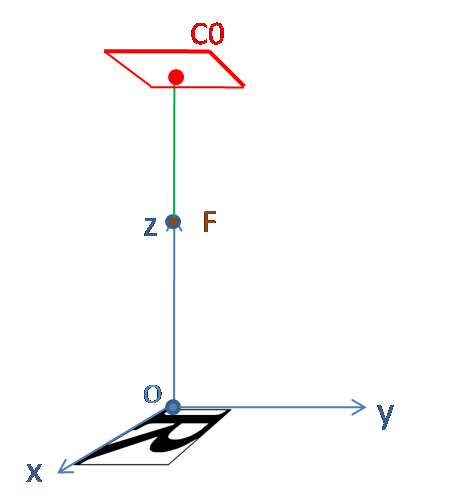
\includegraphics[scale=0.35]{vue_tps_identity.png}}}
		\subfigure[After a first rotation (of angle $\phi$)]{
		\centering
		{
\includegraphics[scale=0.24]{vue_fps_rotation_phi.png}}
		{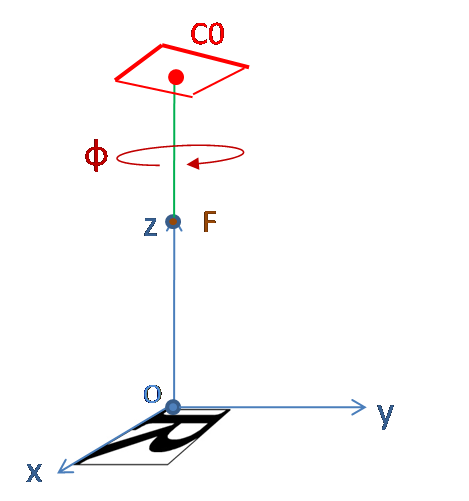
\includegraphics[scale=0.35]{vue_tps_rotation_phi.png}}}
		\subfigure[After the unidirectional homography]{
		\centering
		{
\includegraphics[scale=0.24]{vue_fps_hom_part.png}}
		{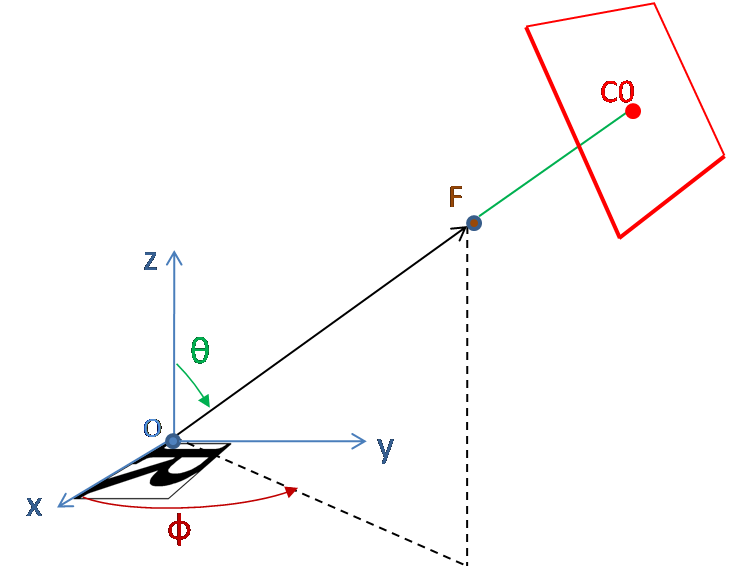
\includegraphics[scale=0.35]{vue_tps_hom_part.png}}}
		\subfigure[Output image (after the rotation of angle  $\psi$)]{
		\centering
		{
\includegraphics[scale=0.24]{vue_fps_rotation_psi.png}}
		{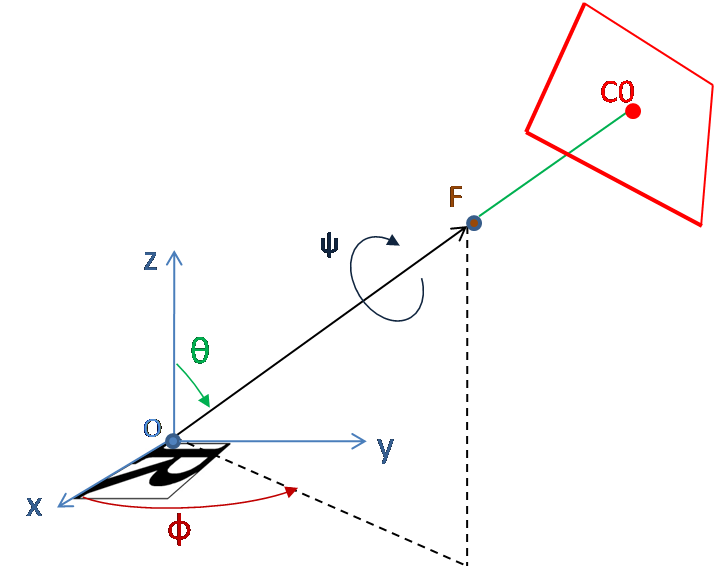
\includegraphics[scale=0.35]{vue_tps_rotation_psi.png}}}
		\caption{Steps to process a homography, represented as camera motion. On the left, the view from the camera, on the right, a motionless representation of the scene. The translations are not represented to simplify the situation. In the motionless views, $F$ is the focus of the camera, the red plane is the image plane of the camera (see section \ref{ref_schema_decomp_cool})}.
		\label{schema_decomp_cool}
		\label{SchemaEtapesDecompoGeometrique}
	\end{figure}
	\clearpage
%simon
		\subsection{Numerical implementation of unidirectional homographies}
			\label{HomoboxRipmap}
			% contient la description des différentes possibilités pour traiter l'homographie unidirectionnelle au centre de la décomposition
%simon
%Homobox refait, une relecture s'impose, manque encore les ref vers les pseudos code (elles sont en com)
%Je sais pas si on doit garder la partie sur l'interp de hermite
\subsubsection{Separation of a unidirectional homography}

By using \eqref{formule_decomposition_effective}, the problem of resampling homographies is reduced to the problem of resampling unidirectional homographies and rotations. This section deals with unidirectional homographies.


%By using formula \ref{formule_decomposition_effective} à traiter des rotations et des homographies unidirectionnelles. Cette section présente une méthode de traitement pour les homograpghies unidirectionnelles.

\label{homobox_paragraph}


Let $h$ be a unidirectional homography 
%On considère une homographie unidirectionelle $h$, de la forme 
\begin{equation*}
h:(x,y)\mapsto \left(\frac{ax+p}{rx+t},\frac{dy+q}{rx+t}\right).
\end{equation*}

Then $h$ can be split in two applications $h_1 , h_2$ defined by
%On peut décomposer cette homographie en deux applications $h_1 , h_2$
\begin{equation*}
h_1:(x,y) \mapsto \left(\frac{ax+p}{rx+t},y\right) \text{ and } h_2:(x,y) \mapsto \left(x,\frac{dy+q}{rx+t}\right),
\end{equation*}
so that $h=h_1  \circ h_2$, allowing the following scheme
\begin{equation*}
f\longrightarrow f'=f\circ h_1 \longrightarrow f''=f'\circ h_2.
\end{equation*}

Each of these mappings is unidimensionnal, resampling each row and each column independently. So the resampling can be computed efficiently :

%Chacune de ces deux transformations ne modifie l'image que dans une seule direction, cela permet d'effectuer des opérations sur des signaux unidimensionnels. Les méthodes de ré-échantillonnage sont donc plus simples, ce qui permet un gain de rapidité car les calculs sont moins coûteux. De plus, les transformations $h_1,h_2$ peuvent être appliquées en ne réalisant que des filtrages horizontaux et verticaux ; les direction de filtrage sont simples.
\begin{itemize}
\item On each column, the first transform is a unidimensional homography.%Sur chaque colonne, la première transformation est une homographie en une dimension.
\item On each row, the second transform is a zoom (which factor is different for each row).%Sur chaque ligne, la seconde transformation est un zoom (d'un facteur différent selon la ligne).
\end{itemize}

The effects of the transforms $h$, $h_1$ and $h_2$ are shown in figure \ref{image_separation_f14}.
%On peut voir sur la figure \ref{image_separation_f14} l'effet des transformations $h,h_1,h_2$.

\begin{figure}[h!]
\centering
\subfigure[identity]{
\includegraphics[scale=0.30]{damier.png}}
\subfigure[unidirectional homography $h=h_1 \circ h_2$]{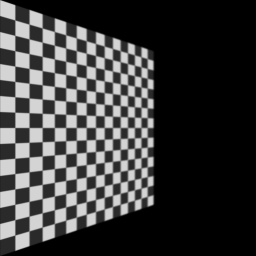
\includegraphics[scale=0.30]{homo_unidirec_f14_2.png}}
\subfigure[transform $h_1$ ]{
\includegraphics[scale=0.30]{homo_unidirec_part_1_f14_2.png}}
\subfigure[transform $h_2$]{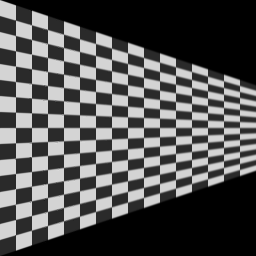
\includegraphics[scale=0.30]{homo_unidirec_part_2_f14_2.png}}
\caption{Separation of a unidirectional homography (scale $0.3$) }
\label{image_separation_f14}
\end{figure}

%\paragraph{Sous-échantillonnage gaussien}
\paragraph{Gaussian downsampling}
\label{zoom_gaussien}
The gaussian zoom is a method of downsampling which uses the convolution $f*G_{d}$, where $G_d$ is a Gaussian kernel of standard deviation $d$. Approximations of the required standard deviation are briefly described in this section, and are based on \emph{is SIFT scale invariant} \cite{morel2011sift}.

%Le zoom gaussien est une méthode de sous-échantillonnage utilisant la convolution $f*G_{d}$ , où $G_d$ est un noyau gaussien d'écart type $d$. Dans nos algorithme on utilisera la méthode développée dans l'article \emph{is SIFT scale invariant} \cite{morel2011sift}.

Let $f$ be an image, assume $f$ is of form $f=G_{c'} * f'$ where $f'$ is an infinite-resolution image. The parameter $c'$ is the Gaussian blur of the image $f$. Experiments show that the ideal blur is $c'=0.8$ \cite{morel2011sift}.\\
Let $z \in [1,+\infty[$, consider $f'_z(x)=f'(zx)$ the downsampled infinite-resolution image.
The Gaussian blur $c$ of the downsampled image $f_z : x \mapsto f(zx)$ has to be $0.8$. To achieve this goal, one may want to convolve $f$ with $G_\sigma$ (with an appropriate standard deviation $\sigma$) before downsample. Since

\begin{equation*}
(f'_z*G_{c})(x)=(f'*G_{cz})(zx)
\end{equation*}
and 
\begin{equation*}
(f*G_\sigma)(zx)=(f'*G_c'*G_\sigma)(zx)=(f'*G_{\sqrt{c'^2 + \sigma^2}})(zx)
\end{equation*}
we conclude
\begin{equation}
\sigma=\sqrt{c^2 z^2 - c'^2}.
\label{formule_zoom_gaussien}
\end{equation}
The parameter $c'$ (the Gaussian blur of the input image) is difficult to compute or to predict. Experiments show that it is between $0.8$ and $0.4$ for reasonably sampled images. A Gaussian blur of $0.7$ in the input image is assumed in our implementation.

%Si $f$ est une image on suppose que $f$ peut s'écrire sous la forme $f=G_{c'} * f'$, où $f'$ est une image de résolution infinie. Le paramètre $c'$ est le facteur de flou gaussien idéal de l'image $f$. L'expérience montre que le facteur de flou gaussien idéal se situe autour de $c=0.8$ \cite{morel2011sift}.\\
%Soit $z\le 1$ posons $f''(x)=f'(zx)$. Si on cherche à échantillonner la fonction  $x\mapsto f(zx)$,  on doit d'abord s'assurer qu'elle possède un facteur de flou gaussien égal à $0.8$. On sait que 

%Grâce à cette relation, on peut en déduire la valeur de $d$ à utiliser, sachant que l'image de départ possède un flou gaussien de $c'$. On obtient

%En identifiant ces deux expressions, on obtient

%Le paramètre $c'$ est difficile à déterminer en pratique. L'expérience montre que pour une image "correctement échantillonnée", le facteur de zoom doit être pris égal à $0.7$. Cependant, pour certaines images provenant de la photographie, on peut prendre $c'=0.5$.

\paragraph{Resampling using integral images}
%\paragraph{Ré-échantillonnage par les images intégrales}
\label{4Integral}

In this paragraph, a method to resample a unidimensional image is presented. This method relies on an approximation of Gaussian blurs using integral images.%(cf. \ref{zoom_gaussien})

%Dans ce paragraphe on présente une méthode permettant de ré-échantillonner une image 1D ; cette méthode s'appuie sur une approximation du zoom gaussien (cf. \ref{zoom_gaussien}) et utilise les images intégrales.

In the following, we denote $\Gcal_n^d$ the kernel defined by
\begin{equation}
\Gcal_1^d(x)=\frac{1}{d}\mathds{1}_{]-\frac{d}{2},\frac{d}{2}[}(x) \text{ and } \Gcal_{n+1}^d= \Gcal_n^d * \Gcal_1^d .
\label{formule_convol_n_int}
\end{equation}

\begin{prop}
The function $x\mapsto \sqrt{n}~\Gcal_n^d(\sqrt{n}~x)$ converges uniformly on $\mathbb{R}$ to a Gaussian function .
\end{prop}

%Soit $\Gcal_n^d$ le noyau définit par 

%Cette suite de fonctions vérifie la propriété suivante
%\begin{prop}
%La fonction $x\mapsto \sqrt{n}~\Gcal_n^d(\sqrt{n}~x)$ converge uniformément sur $\mathbb{R}$ vers une courbe gaussienne 
%\end{prop}
\begin{figure}
\centering
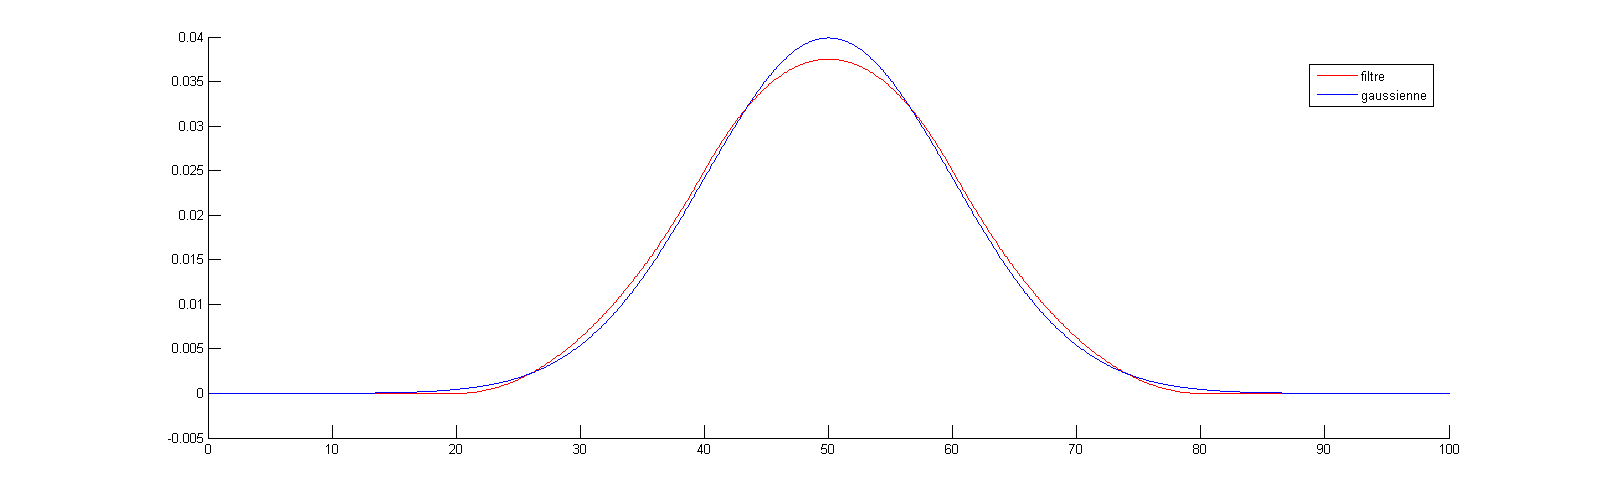
\includegraphics[width=15cm]{filtre_g3.png}
\caption{Comparison between $\Gcal_3^{20}$ and $G_{10}$ (centered on $50$)}
\end{figure}

From now on we denote $D_d$ the ''discret differentiation'' operator defined by $D_d f(x)=\frac{f(x+\frac{d}{2})-f(x-\frac{d}{2})}{d}$ and if $f$ is a compactly supported piecewise continuous function, we denote \begin{equation*}
F_{n+1}(x)= \int_{-\infty}^{x}F_{n}(y)dy~~~ \txt{ and }~~~F_{0}(x)= f(x).
\end{equation*}

Then, we have the following proposition for the continuous case :

\begin{prop} If $f$ is a compactly supported piecewise continuous function then
\begin{equation}
 (f*\Gcal_n^d)(y)=D_d^n F_{n}(y)= \frac{1}{d^n}\underset{0 \le k\le n}{\sum} \binom{n}{k}(-1)^{k} F_{n}(y+\frac{(n-2k)d}{2}).
\end{equation}
\label{continuous_approx}
\end{prop}



%Si $f$ est une fonction continue par morceaux on définit $D_d$ l'opérateur de "dérivation discrète" par $D_d f(x)=\frac{f(x+\frac{d}{2})-f(x-\frac{d}{2})}{d}$  et on pose

%On a alors lemme suivant 

\begin{proof}
Let $f$ be a compactly supported piecewise continuous function, then
\begin{eqnarray*}
(f * \Gcal_1^d )(y)&=&\frac{1}{d} \int_{[y-\frac{d}{2},y+\frac{d}{2}]} f(x) dx\\
               &=&\frac{F_{1}(y+\frac{d}{2})-F_{1}(y-\frac{d}{2})}{d}\\
               &=&D_d F_{1}(y)
\end{eqnarray*}


\noindent Let's prove by induction on $n$ that $ f*\Gcal_n^d=D_d^n F_{n}$.\\
It is true for $n=1$. If it is true for $n$ then
\begin{equation*}
f*\Gcal_{n+1}^{d}=(f * \Gcal_{n}^d) * \Gcal_{1}^{d}= (D_d^n F_{n})*\Gcal_1^d.
\end{equation*}
By linearity of the convolution
\begin{equation*}
(f*\Gcal_{n+1}^{d}) = D_d^n (F_{n}*\Gcal_1^d) = D_d^{n+1} F_{n+1}.
\end{equation*}
$D_d^n$ is the sum of translation operators
\begin{equation*}
f\mapsto f(\cdot+\frac{d}{2})~~~\txt{ and }~~~f\mapsto f(\cdot-\frac{d}{2})?
\end{equation*}
so it can be developed using a binomial formula. Therefore

%On peut développer $D_d^n$ à l'aide du binome de Newton car les deux opérateurs commutent. On obtient donc
\begin{equation*}
(f*\Gcal_n^d)(y) = \frac{1}{d^n}\underset{0 \le k\le n}{\sum} \binom{n}{k}(-1)^{k} F_{n}(y+\frac{(n-2k)d}{2}).
\end{equation*}
\end{proof}


%In the implementation, the computation of $D_d^n$ is done by induction (see algorithm \ref{pseudo_code_convol_4_int}).

An approximation of $F_{k}$ is required in order to adapt proposition \ref{continuous_approx} to a discrete signal and use these formulas.\\
\medbreak
Let $(f_k)_{k=0...m-1}$ be a discrete signal, define $(F_n)$ the piecewise polynomial interpolation of degree $n$ by

\begin{equation}
F_{0} (x) =\underset{0\le k \le m-1}{\sum}f_{k} \mathds{1}_{[k,k+1[}(x) \txt{ and }  F_{n}(x)=\int_{-\infty}^{x}F_{n-1}(y)dx.
\label{defintion_fn}
\end{equation}

\noindent Then $F_{n}$ can be computed for every $n\in\mb{N}$ : for $n=1$,

\begin{equation*}
F_{1}(x)=\underset{k\le \lfloor x\rfloor \wedge m-1}{\sum}f_{k}+ f_{\lfloor x\rfloor}
(x-\lfloor x\rfloor)
\end{equation*}

\noindent This function is a piecewise affine map. It can be shown by induction on $n\geq 1$ that

\begin{eqnarray*}
F_{n}(x)
&=&
F_n(\lfloor x\rfloor) + \displaystyle{\sum_{0 \leq k \leq n-1}}F_{k}(\lfloor x \rfloor) \frac{(x-\lfloor x \rfloor)^{n-k}}{(n-k)!} \text{ if } x<m\\
&=&
F_{n}(m) + \displaystyle{\sum_{1 \leq k \leq n-1}} F_{k}(m) \frac{(x-m)^{n-1-k}}{(n-1-k)!} \text{ if } x \geq m
\end{eqnarray*}

\noindent where values of $F_n(\lfloor x\rfloor)$ can be computed by induction using

\begin{equation*}
\forall k \in \llbracket 0 ; m-1 \rrbracket, F_{n}(k+1)=F_{n}(k)+\underset{0\le l \leq n-1}{\sum} \frac{F_{l}(k)}{(n-l)!}
\end{equation*}

%Dans nos algorithmes, on utilisera généralement cette propriété pour $n=3$ mais on calculera l'opérateur $D_d^n$ en faisant des différences successives (algorithme \ref{pseudo_code_convol_4_int}).

%On doit cependant calculer une valeur approchée des fonctions $F_{k}$  car on ne connait que les échantillons de la fonctions $f$.\\
%Si le signal discret possède $m$ valeurs non nulles $f_k,k=0...m-1$, on peut poser 


%Cette fonction est affine par morceaux. On peut démontrer la formule suivante par récurrence

%Où la valeur de $F_{n}$ se calcule par récurrence :

\noindent So the values on integers and the value of a polynomial of degree $n$ has to be computed to interpolate on non-integers.

\medbreak
With this method the signal $(f_k)$ could be resampled by interpolating it with $F_{0}$ in the first place, and then by convolving with a kernel $\Gcal_n^d$.

\noindent But when this method is used, the image is initially interpolated with a piecewise constant function, and when $d$ is small, resampling using $F_{0}*\Gcal_n^d$ is equivalent to resampling using the value of the closest point. However this problem can be solved by convolving initially with $\Gcal_1^1$, and therefore considering a piecewise affine interpolation $\tilde F = F_0*\Gcal_1^1$ of the samples $(f_k)$.

%Dans cette méthode on ré-échantillonne le signal $(f_k)$ en l'interpolant d'abord par la fonction $F_{0}$, puis on ré-échantillonne en appliquant une convolution avec un noyau $\Gcal_n^d$. On utilise dans nos algorithmes les fonctions $\Gcal_3^d$ car elles se sont de bonnes approximations de courbes gaussiennes.\\ %placer figure 
%Dans cette méthode, l'image est initialement interpolée par une fonction constante par morceaux. Lorsque le paramètre $d$ est choisi très petit, le ré-échantillonnage $F_{0}*\Gcal_3^d$ est équivalent à la méthode du point le plus proche.\\
%On peut cependant corriger ce problème


%JUJUJU

\begin{prop}
Let $(f_k)$ be a discrete signal, $(F_n)$ defined by \eqref{defintion_fn} and $\tilde F$ its piecewise affine interpolation. Then
\begin{equation*}
( \tilde{F} * \Gcal_n^d ) (x) = D_d^{n}D_1 F_{n+1}(x).
\end{equation*}
\end{prop}

\begin{proof}
We have
\begin{equation*}
\tilde{F}(x)=(F_{0} * \Gcal_1^1 )(x),
\end{equation*}
so
\begin{equation*}
\tilde{F}*\Gcal_n^d=F_{0}*\Gcal_1^1*\Gcal_n^d=F_{0}*\Gcal_n^d*\Gcal_1^1=(D_d^n F_{n})*\Gcal_1^1=D_d^n (F_{n}*\Gcal_1^1)= D_d^n (D_1 F_{n+1}).
\end{equation*}
\end{proof}


The additional interpolation can be obtained by evaluating $F_{n+1}$.
It is possible to use this method to have a more regular representation of the input signal, but $F_0 * \Gcal_p^1~$ is not exact on the integers if $2\le p$.\\
In practice the implementation uses $\Gcal_3^d * \Gcal_1^1$, and therefore approximations of $F_n$ for $n=1...4$ are required.



To compute the values of $F_n$ for $n=1...4$, values on integers are precomputed and then polynomials are evaluated.


To precompute the values on integers, the relations
\begin{eqnarray}
F_{1}(k+1)&=&  F_{1}(k)+f_{k}, \label{formula_discret_integral_1}\\
F_{2}(k+1)&=&  F_{2}(k)+F_{1}(k)+\frac{f_{k}}{2}, \label{formula_discret_integral_2}\\
F_{3}(k+1)&=&  F_{3}(k)+F_{2}(k)+\frac{F_{1}(k)}{2}+\frac{f_{k}}{6}, \label{formula_discret_integral_3}\\
F_{4}(k+1)&=&  F_{4}(k)+F_{3}(k)+\frac{F_{2}(k)}{2}+\frac{F_{1}(k)}{6}+\frac{f_{k}}{24}, \label{formula_discret_integral_4}
\end{eqnarray}
are used (see algorithm \ref{pseudo_code_built_4_int}).


%On doit calculer une composante constante par morceaux afin d'avoir la valeur de $F_{n}$ aux entiers ainsi qu'un terme polynomial de degré $n$ pour effectuer l'interpolation sur des valeurs non-entières.

To compute values on non-integers, the following scheme is used :

\begin{itemize}
\item If $x\le 0$ then
\begin{equation}
\label{formula_nonint_integral_case1}
F_{4}(x)=0.
\end{equation}
\item If $x\in ]0 , m[$ then
\begin{equation}
\label{formula_nonint_integral_case2}
F_{4}(x)-F_{4}(\lfloor x \rfloor)=P_{\lfloor x \rfloor}(x-\lfloor x \rfloor)
\end{equation}
where $P_k$ is a polynomial of degree $4$ defined by
\begin{equation*}
P_k (r) =r \left( F_{3}(k) +\frac{r}{2} \left(F_{2}(k)+ \frac{r}{3}\left(F_{1}(k)+\frac{r}{4} f_{k}\right)\right)\right), k=0...m-1.
\end{equation*}
\item If $x\ge m$ then
\begin{equation}
\label{formula_nonint_integral_case3}
F_{4}(x)-F_{4}(m)=Q(x-m)
\end{equation}
where  $Q$ is a polynomial of degree 3 defined by
\begin{equation*}
Q(r)=r \left(F_{3}(m)+\frac{r}{2} \left( F_{2}(m) + \frac{r}{3} F_1 (m)\right)\right).
\end{equation*}\
\end{itemize}

These formulas are used in the algorithm \ref{pseudo_code_eval_4_int}.

%Dans la pratique, on a utilisé cette formule pour $n=4$. Afin d'évaluer $F_4$, on procède de la façon suivante 

%Ces formules sont utilisées dans l'algorithme permettant d'évaluer l'intégrale quatrième de l'image (algorithme \ref{pseudo_code_eval_4_int}).

%Pour calculer la valeur $F_4$ aux entiers, on peut applique la relation de récurrence suivante

%Ces formules sont utilisées dans le pseudo-code (algorithme \ref{pseudo_code_built_4_int}).


\medbreak


To implement this method, the parameter $d$ has to be chosen with respect to the local zoom $z$ in the point considered. The zoom factor $z$ is given by the derivative of the transform.\\
The results from the previous paragraph (cf. \ref{zoom_gaussien}) are used since $\Gcal_3^d$ is a good approximation of a Gaussian function. According to Wells \cite{wells1986efficient}, the parameter $d$ so that $\Gcal_3^d$ approximates $G_\sigma$ should check $\sigma^2 = \frac 1 4 \left((d+1)^2-1\right)$. Thus, for $z \geq 1$, by \eqref{formule_zoom_gaussien}

\begin{equation*}
d=\sqrt{2(c^2 z^2 - c'^2)+1}-1 \text{ with } c=0.8 \text{ and } c'=0.7.
\end{equation*}

The value of $c'$ is fixed to $0.7$ in our implementation, but it could be chosen accordingly to the input image : for sharp image, it has to be around $0.5$ to avoid aliasing. A too small value introduces an excessive blur.

%L'interpolation supplémentaire peut donc être obtenue en évaluant $F_{n+1}$. La méthode de calcul est donc la même que dans le cas précédent, la convolution avec $\Gcal_3^d$ nécessite l'utilisation l'intégrale quatrième de l'image dans la pratique.\\
%Il est possible d'utiliser cette méthode pour obtenir une représentation plus régulière du signal de départ mais la courbe $F_0 * \Gcal_p^1~$ n'est pas interpolante si $2\le p$.\\
%à faire mieux 
%Afin d'implémenter cette méthode, nous devons déterminer la valeur du paramètre $d$ en fonction du facteur de zoom local $z$ que l'on doit effectuer en ce point. $z$ sera choisi égal à la dérivé de la transformation au point où l'on ré-échantillonne.\\ 
%On réutilise les résultats du paragraphe précédent (cf. \ref{zoom_gaussien}), car les  fonctions $\Gcal_3^d$ sont de bonnes approximations de courbes gaussiennes. L'écart type $\sigma$ de $\Gcal_3^d$ est donné par la formule 

%Par la formule du zoom gaussien (formule \ref{formule_zoom_gaussien}), on en déduit que si $z\ge 1$, alors

%La valeur de $c'$ peut être choisie en fonction de l'image d'entrée : pour des images très nettes, si l'on souhaite que le résultat final ne soit pas aliasé, on doit prendre une valeur de $c'$ autour de $0.5$. Pour la majorité des image utilisée lors de nos expériences une valeur de $0.7$ était suffisante. Une valeur trop faible de $c'$ aboutit à un flou excessif.
%simon
		%\subsection{A method for rotations} %placé dans la partie experiments
			\label{YaroSzeli}
			%% contient la description des différentes méthodes pour traiter les rotations de la décomposition

There are numerous methods to process the two rotations of the geometric decomposition. In addition to the multi-pass resampling method for affinity \cite{szeliski2010high}, the method in Fourier due to Yaroslavky \cite{unser1995convolution} is well-known for its efficiency. This section briefly compares the two. The multi-pass method has also numerous alternatives since it is a decomposition which allow several interpolation methods. Here convolutions with a raised cosine-weighted sinc and interpolations with splines are compared.




%Pour les deux rotations dans la décomposition, plusieurs méthodes sont possibles : en plus de la méthode de traitement des affinités multi-étapes \cite{szeliski2010high}, la méthode de Yaroslavsky \cite{unser1995convolution} est connue pour son efficacité à traiter les rotations. On cherchera donc à les comparer. La méthode multi-étapes n'étant qu'une décomposition d'une affinité en quatre opérations, la comparaison se fera aussi entre plusieurs implémentations de cette méthode, en faisant varier la manière d'interpoler (convolution par un \emph{raised cosine-weighted sinc}, interpolation par des splines).

Theoretically it is not correct to use splines here since the decompositon has been conceived for filtering with $h(\frac{\dot{}}{s})$ which has a variable support. However with rotations $u_{max}=v_{max}=1$, so the parameter $s$ does not impact the two first call to $\mathcal R$. If the rotation has a small angle, $r_v$ and $r_h$ are close to 1, so $s$ has very little impact, and the generally variable support is constant. In this case there is no theoretical problem.

The results are shown figure \ref{troiscentrotations} and \ref{rotalena}. The multi-pass method is used in the algorithms.


%Il est théoriquement incorrect d'utiliser des splines pour cette interpolation (on rappelle qu'on convole avec $h(\frac{\dot{}}{s})$ pour filtrer les fréquences voulues ; le support du filtre est adaptatif). Cependant, dans le cas des rotations, $u_{max}$ et $v_{max}$ valent 1, donc le paramètre $s$ n'a pas d'influence sur les deux premiers $\mathcal R$. Si de plus la rotation est d'angle faible, $r_v$ et $r_h$ sont proches de 1, donc $s$ a très peu d'influence. Donc dans ce dernier cas, convoler avec un filtre à support adaptatif (qui sera finalement un support fixé) ou interpoler par des b-splines ne change rien au niveau théorique.
 %Jean-Thomas a fait une partie sur Yaroslavsky...
	\clearpage
	\section*{Conclusion}
			%ici une conclusion chouette

%La décomposition géométrique permet ainsi une réalisation des homographies de meilleure qualité, et un contrôle plus rigoureux de l'\emph{aliasing} et du flou introduits. Les solutions proposées ici pour implémenter les différentes étapes ne sont que des exemples. Elles sont coûteuses en calcul bien que linéaires. Cependant, chaque étape n'agit que sur les lignes ou que sur les colonnes, ce qui permet une parallélisation efficace.

%On peut ainsi imaginer des approximations moins satisfaisantes mais beaucoup plus rapides, par exemple en utilisant une méthode triple intégrale pour les rotations. De même le traitement de l'homographie unidirectionnelle peut-être simplifié, par exemple en n'intégrant que sur les entiers et en réalisant une interpolation bilinéaire.

%A l'inverse si le temps de calcul n'est pas critique on peut utiliser des splines d'ordre élevé pour les rotations, ou même lors du traitement de l'homographie unidirectionnelle.

%On a ainsi proposé une décomposition géométrique des homographies autour de laquelle de nombreux algorithmes peuvent s'articuler.






The geometric decomposition allows a resampling by homography of higher quality and a stricter control of introduced aliasing and blurring. The solutions presented here to implement each step are computationally intensive but they are linear (with respect to the number of pixels) and since they act independently on rows or on columns, they can by efficiently parallelized.

There can still be less rigorous but faster approximations, for example by adapting the 4-integral image for the multi-pass resampling of rotations. The resampling of the unidirectional homography can also be simplified, for example by integrating only on integers and using bilinear interpolation between them.

On the contrary, if computational time is not important, splines of high order can be used to resample the unidirectional homography.

To conclude, we have proposed a geometric decomposition of homographies on which a lot of algorithms can be based.

	\clearpage
	\section{Experiments}
		\label{experiences}
		Our experiments were implemented in C. First the spectral behaviour of the multi-pass resampling method for an affine transform was checked. Then the new geometric method was compared to the Ripmap.

%On présente ici des expériences réalisées en C. On vérifie d'abord le comportement spectral du traitement multi-étape d'une affinité. On compare ensuite la nouvelle méthode au Ripmap.

\subsection{Multi-pass resampling method for an affine transform}

%\subsection{Décomposition multi-étapes d'une affinité}
 
 
 The results of multi-pass resampling method for an affine transform \cite{szeliski2010high} (part \ref{szeliski_section}) as well as the image's spectrum at the successive steps are examined in this section. The affine transform being here a shear, the decomposition has three basic steps, instead of four for a general affine transform.  
 
 %On présente ici les résultats de la décomposition multi-étapes d'une affinité \cite{szeliski2010high} (section \ref{szeliski_section}), ainsi que le spectre de l'image aux différentes étapes. L'affinité utilisée étant elle-même un \emph{shear}, la décomposition se réduit à trois étapes élémentaires, au lieu des quatres d'une affinité quelconque.
 \begin{figure}
		\centering
		\subfigure[Initial image (scale 3/8)]{
			{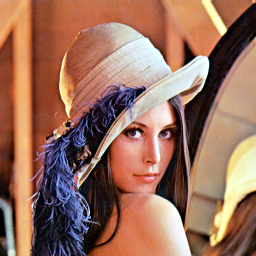
\includegraphics[scale=0.375]{decompoSzeliski_sinc_image_entree.png}}
			{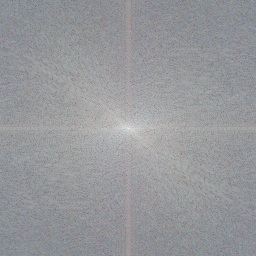
\includegraphics[scale=0.375]{decompoSzeliski_sinc_fourier_entree.png}}
		}
		\subfigure[Initial image in a nine times larger one (scale 1/8)]{
			{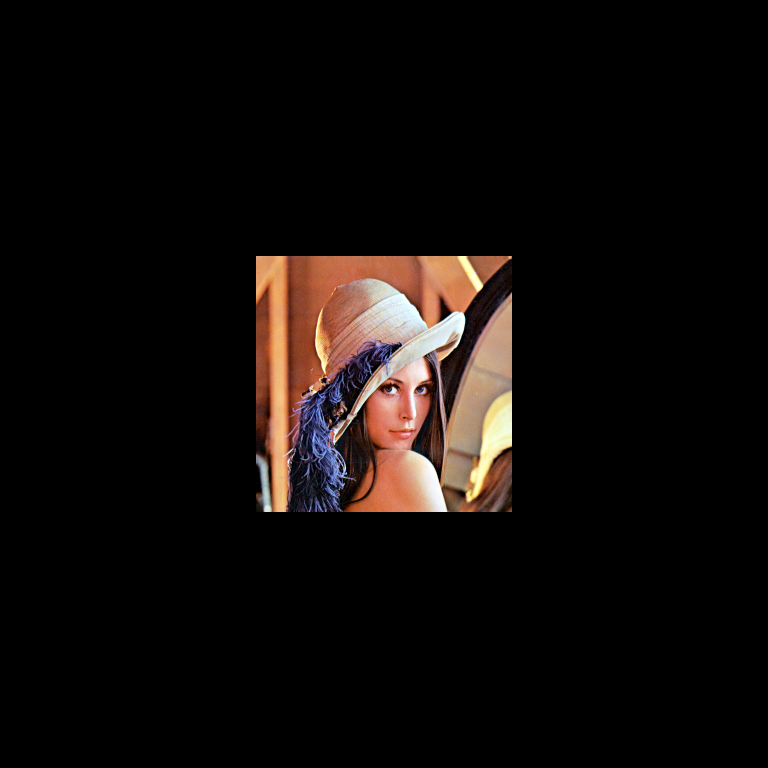
\includegraphics[scale=0.125]{decompoSzeliski_sinc_image1.png}}
			{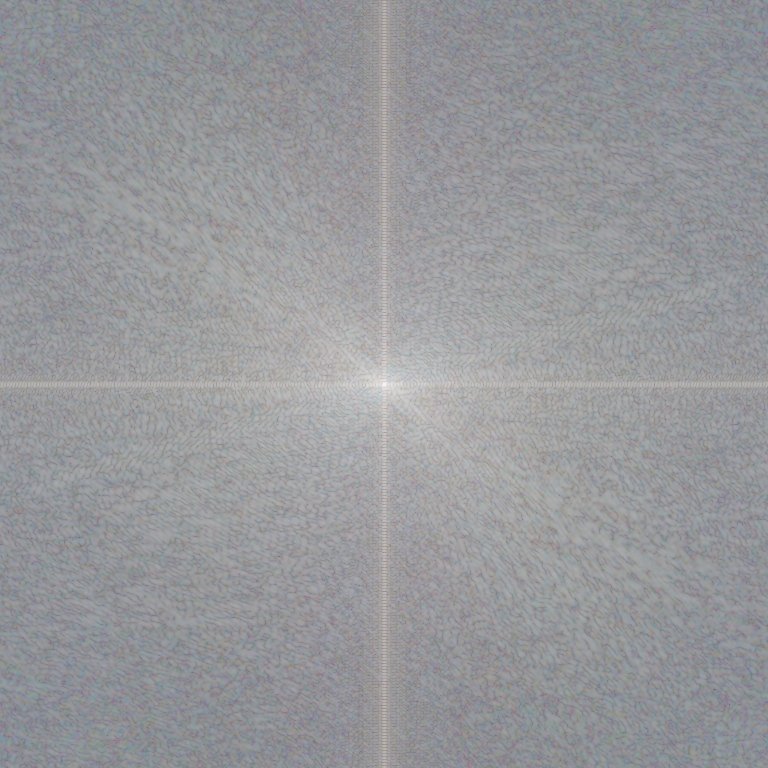
\includegraphics[scale=0.125]{decompoSzeliski_sinc_fourier1.png}}
		}
		\subfigure[After the first $\mathcal R$ (scale 1/8)]{
			{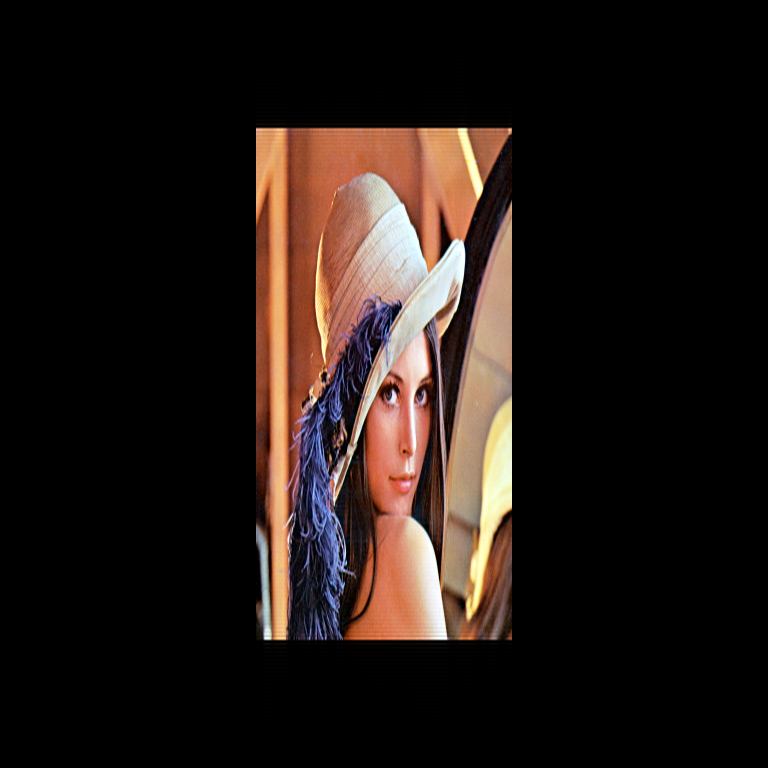
\includegraphics[scale=0.125]{decompoSzeliski_sinc_image2.png}}
			{
\includegraphics[scale=0.125]{decompoSzeliski_sinc_fourier2.png}}
		}
		\subfigure[After the second $\mathcal R$ (scale 1/8)]{
			{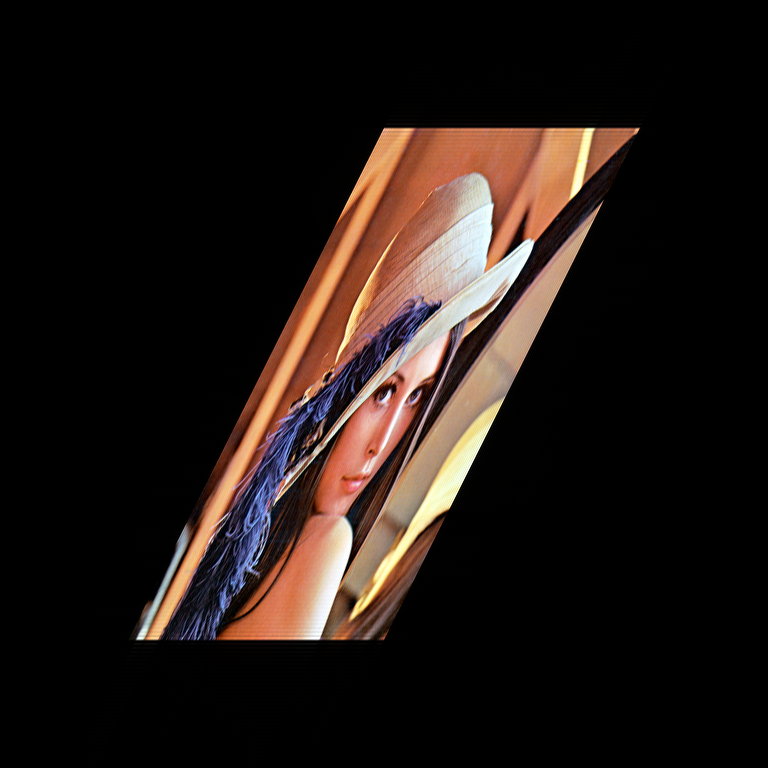
\includegraphics[scale=0.125]{decompoSzeliski_sinc_image3.png}}
			{
\includegraphics[scale=0.125]{decompoSzeliski_sinc_fourier3.png}}
		}
		\subfigure[After the third $\mathcal R$ (scale 1/8)]{
			{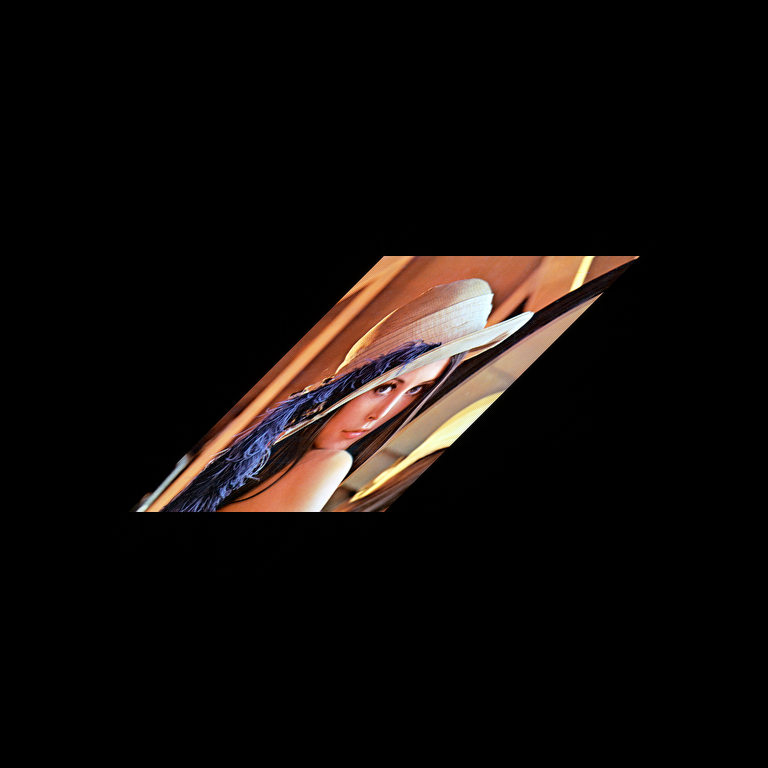
\includegraphics[scale=0.125]{decompoSzeliski_sinc_image4.png}}
			{
\includegraphics[scale=0.125]{decompoSzeliski_sinc_fourier4.png}}
		}
		\subfigure[Final image (scale 3/8)]{
			{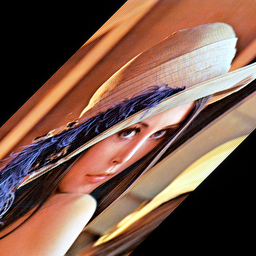
\includegraphics[scale=0.375]{decompoSzeliski_sinc_image_sortie.png}}
			{
\includegraphics[scale=0.375]{decompoSzeliski_sinc_fourier_sortie.png}}
		}
		\caption{Steps of the multi-pass resampling method for an affine transform explained in section \ref{szeliski_section} (on the left is the image at each steps, on the right is the logarithm of the modulus of the Fourier transform of this image). The interpolation filter is a sinc function (with period 1). To appreciate the quality of the final result it is advised to zoom  it in by a factor 3.}
		\label{experiments_decompoSzeliski_sinc}
	\end{figure}
	%\begin{figure}
	%	\centering
	%	\subfigure[Image initiale (échelle 3/8)]{
	%		{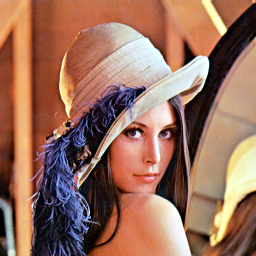
\includegraphics[scale=0.375]{decompoSzeliski_sinc_image_entree.png}}
	%		{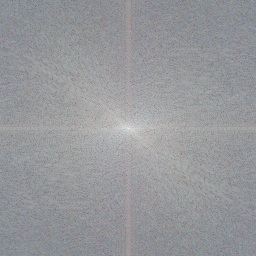
\includegraphics[scale=0.375]{decompoSzeliski_sinc_fourier_entree.png}}
	%	}
	%	\subfigure[Image plongée dans une image neuf fois plus grande (échelle 1/8)]{
	%		{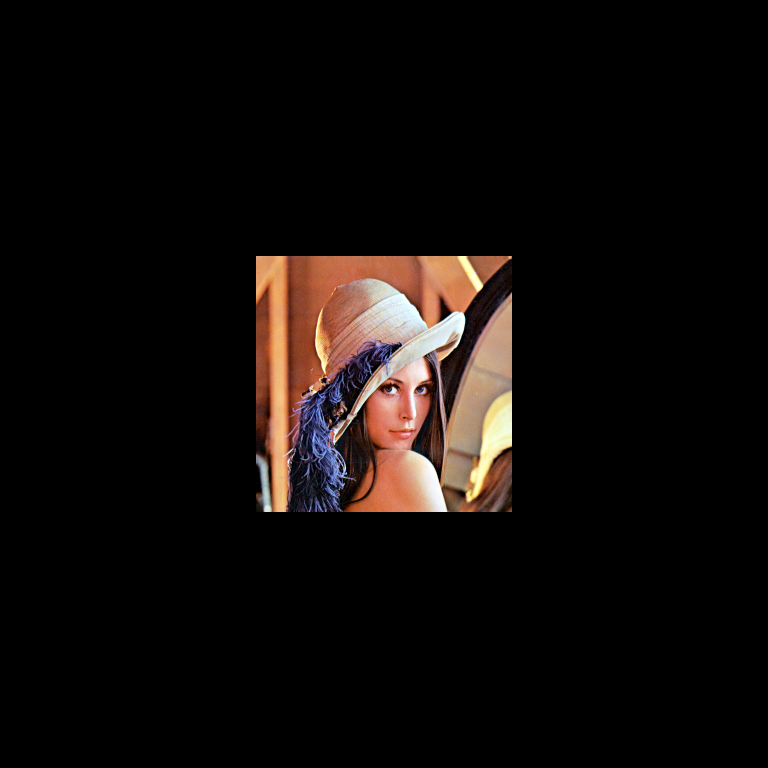
\includegraphics[scale=0.125]{decompoSzeliski_sinc_image1.png}}
	%		{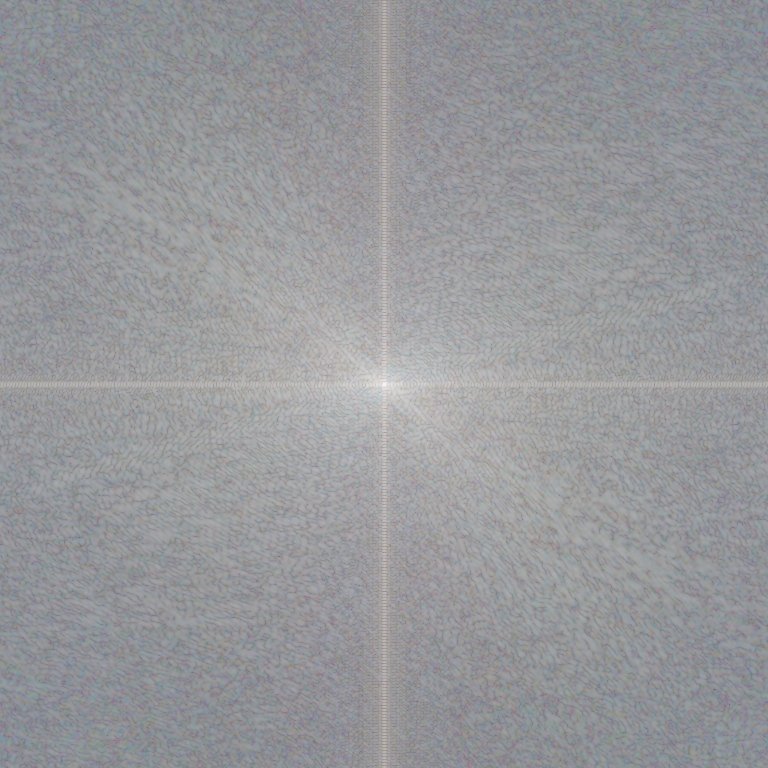
\includegraphics[scale=0.125]{decompoSzeliski_sinc_fourier1.png}}
	%	}
	%	\subfigure[Après le premier $\mathcal R$ (échelle 1/8)]{
	%		{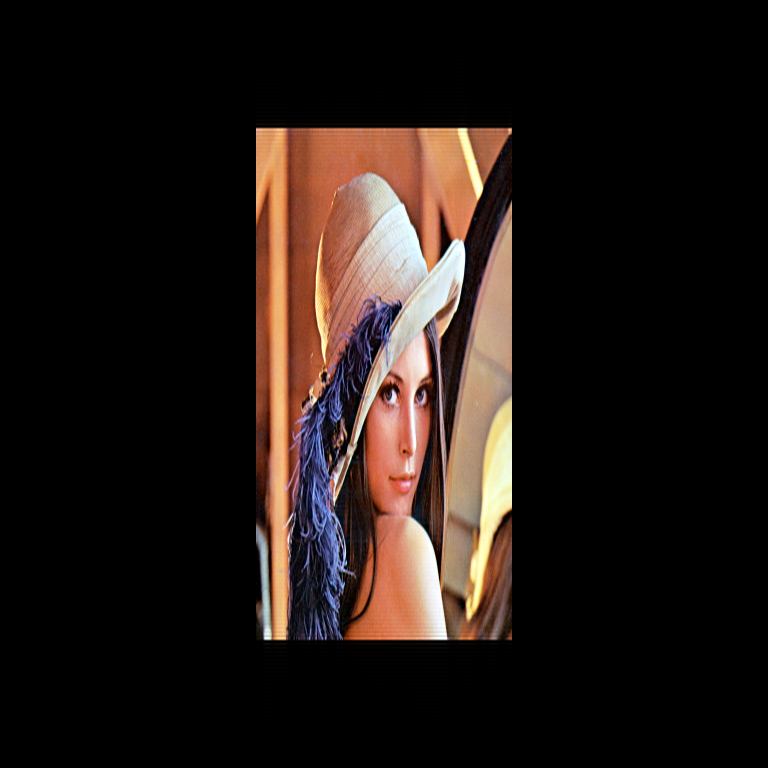
\includegraphics[scale=0.125]{decompoSzeliski_sinc_image2.png}}
	%		{
\includegraphics[scale=0.125]{decompoSzeliski_sinc_fourier2.png}}
	%	}
	%	\subfigure[Après le deuxième $\mathcal R$ (échelle 1/8)]{
	%		{\includegraphics[scale=0.125]{decompoSzeliski_sinc_image3.png}}
	%		{\includegraphics[scale=0.125]{decompoSzeliski_sinc_fourier3.png}}
	%	}
	%	\subfigure[Après le troisième $\mathcal R$ (échelle 1/8)]{
	%		{\includegraphics[scale=0.125]{decompoSzeliski_sinc_image4.png}}
	%	}
	%	\subfigure[Image finale (échelle 3/8)]{
	%		{\includegraphics[scale=0.375]{decompoSzeliski_sinc_image_sortie.png}}
	%		{\includegraphics[scale=0.375]{decompoSzeliski_sinc_fourier_sortie.png}}
	%	}
	%	\caption{Étapes du traitement des affinités présenté en \ref{szeliski_section} (à gauche l'image à chaque étape, à droite le logarithme du module de la transformée de Fourier de cette image). Le filtre d'interpolation est un \emph{sinc} (de période 1)}
	%	\label{experiments_decompoSzeliski_sinc}
	%\end{figure}
	For figure \ref{experiments_decompoSzeliski_sinc}, we used  a raised cosine-weighted sinc filter of the form (see formula \eqref{szeliski_definition_raisedCosineWeightedSinc}) 
		\[h : x \mapsto \sinc(\frac{x}{T})\frac{\cos(\frac{\pi\beta x}{T})}{1-\frac{4\beta^2x^2}{T^2}}\].
		There is no loss of visual quality if one reduces the convolution with this filter to a large enough finite number of terms.
		
	%En figure \ref{experiments_decompoSzeliski_sinc}, le filtre utilisé est un \emph{sinc}, correspondant au \emph{raised cosine-weighted sinc} avec $\beta = 0$ ; pour rappel, le filtre a pour forme
	%\[h : x \mapsto \sinc(\frac{x}{T})\frac{\cos(\frac{\pi\beta x}{T})}{1-\frac{4\beta^2x^2}{T^2}}\]
	%On ne perd pas en qualité visuelle en réduisant la convolution à un nombre fini de termes suffisamment grand.

 	\begin{figure}
		\centering
		\subfigure[Initial image (scale 3/8)]{
			{\includegraphics[scale=0.375]{decompoSzeliski_image_entree.png}}
			{\includegraphics[scale=0.375]{decompoSzeliski_fourier_entree.png}}
		}
		\subfigure[Inital image in a nine times larger one (scale 1/8)]{
			{\includegraphics[scale=0.125]{decompoSzeliski_image1.png}}
			{\includegraphics[scale=0.125]{decompoSzeliski_fourier1.png}}
		}
		\subfigure[After the first $\mathcal R$ (scale 1/8)]{
			{\includegraphics[scale=0.125]{decompoSzeliski_image2.png}}
			{\includegraphics[scale=0.125]{decompoSzeliski_fourier2.png}}
		}
		\subfigure[After the second $\mathcal R$ (scale 1/8)]{
			{\includegraphics[scale=0.125]{decompoSzeliski_image3.png}}
			{\includegraphics[scale=0.125]{decompoSzeliski_fourier3.png}}
		}
		\subfigure[After the third $\mathcal R$ (scale 1/8)]{
			{\includegraphics[scale=0.125]{decompoSzeliski_image4.png}}
			{\includegraphics[scale=0.125]{decompoSzeliski_fourier4.png}}
		}
		\subfigure[Final image (Scale 3/8)]{
			{\includegraphics[scale=0.375]{decompoSzeliski_image_sortie.png}}
			{\includegraphics[scale=0.375]{decompoSzeliski_fourier_sortie.png}}
		}
		\caption{Steps of the multi-pass resampling method for an affine transform explained in section \ref{szeliski_section} (on the left is the image at each step, on the right is the logarithm of the modulus of the Fourier transform of this image). The interpolation filter is a raised cosine-weighted sinc (with period 1 and with a roll-off factor $\beta = 0.25$).To appreciate the quality of the final result it is advised to zoom  it in by a factor 3. Compare with Figure \ref{experiments_decompoSzeliski_sinc}.}
		\label{experiments_decompoSzeliski}
	\end{figure}

	%\begin{figure}
	%	\centering
	%	\subfigure[Image initiale (échelle 3/8)]{
	%		{\includegraphics[scale=0.375]{decompoSzeliski_image_entree.png}}
	%		{\includegraphics[scale=0.375]{decompoSzeliski_fourier_entree.png}}
	%	}
	%	\subfigure[Image plongée dans une image neuf fois plus grande (échelle 1/8)]{
	%		{\includegraphics[scale=0.125]{decompoSzeliski_image1.png}}
	%		{\includegraphics[scale=0.125]{decompoSzeliski_fourier1.png}}
	%	}
	%	\subfigure[Après le premier $\mathcal R$ (échelle 1/8)]{
	%		{\includegraphics[scale=0.125]{decompoSzeliski_image2.png}}
	%		{\includegraphics[scale=0.125]{decompoSzeliski_fourier2.png}}
	%	}
	%	\subfigure[Après le deuxième $\mathcal R$ (échelle 1/8)]{
	%		{\includegraphics[scale=0.125]{decompoSzeliski_image3.png}}
	%		{\includegraphics[scale=0.125]{decompoSzeliski_fourier3.png}}
	%	}
	%	\subfigure[Après le troisième $\mathcal R$ (échelle 1/8)]{
	%		{\includegraphics[scale=0.125]{decompoSzeliski_image4.png}}
	%		{\includegraphics[scale=0.125]{decompoSzeliski_fourier4.png}}
	%	}
	%	\subfigure[Image finale (échelle 3/8)]{
	%		{\includegraphics[scale=0.375]{decompoSzeliski_image_sortie.png}}
	%		{\includegraphics[scale=0.375]{decompoSzeliski_fourier_sortie.png}}
	%	}
	%	\caption{Étapes du traitement des affinités présenté en \ref{szeliski_section} (à gauche l'image à chaque étape, à droite le logarithme du module de la transformée de Fourier de cette image). Le filtre d'interpolation est un \emph{raised cosine-weighted sinc} (de période 1, de \emph{roll-off factor} $\beta = 0.25$)}
	%	\label{experiments_decompoSzeliski}
	%\end{figure}

		\clearpage
		%\subsubsection*{Comparaison entre la méthode de Yaroslavsky et la méthode de traitement des affinités multi-étapes}

\subsection{Comparison between Yaroslavsky's method and the multi-pass resampling method}

	In the following experiments, the RMSE (Root Mean Square Error) is the $L^2$ norm of the difference between the initial image and the final image, the MAE (Mean Absolute Error) is the $L^1$ norm of this difference and the maximal error is the maximum ($L^\infty$ norm) of this difference.\\


There are numerous methods to process the two rotations of the geometric decomposition. In addition to the multi-pass resampling method for affine maps \cite{szeliski2010high}, the method in Fourier due to Yaroslavky \cite{unser1995convolution} is well-known for its efficiency. They are compared through an experiment figure \ref{rotalena} : beginning from the original image, 10 rotations of 36 degrees are processed using different methods (including the naive linear interpolation).

 \begin{figure}[h!]
   \centering
   \subfigPDP{original lena.png}{lena.png}
   \subfigPDP{lena.png after 10 rotations by linear interpolation}{linear_10rot_lena.png}
   \subfigPDP{lena.png after 10 rotations by the multi-pass resampling method (interpolation filter : raised cosine-weighted sinc)}{lena_10_rotations_szeli.png}
   \subfigPDP{lena.png after 10 rotations by Yaroslasky's method}{lena_10_rotations_yaro.png}
   \subfigPDP{difference between lena.png and lena.png after ten rotations by multi-pass resampling method (interpolation filter : raised cosine-weighted sinc)}{raised-cosine_beta0_36_10rot_lena_error.png}
   \subfigPDP{difference between lena.png and lena.png after 10 rotations by Yaroslasky's method}{lena_10_rotations_yaro_error.png}
 \subfigure[Errors on 10 rotations of 36 degrees]{\begin{tabular}{|c|c|c|c|c|}
  \hline
  Method & RMSE  & MAE & maximal error  \\
  \hline
  linear interpolation & 14.722 & 8.5485 & 147.43  \\
  Yaroslavsky's method & 12.817 & 7.3749 & 159.84  \\
  multi-pass resampling &   \bf{5.9791} & \bf{3.6243} & \bf{72.129} \\
  \hline
 \end{tabular}}
 \caption{Effect for 10 rotations (see section \ref{pleinsderotations})}
 \label{rotalena}
 \end{figure}
 
 The multi-pass resampling method using raised cosine-weighted sinc as interpolation filter and Yaroslavsky's method seem perfect.\\

	To enhance the difference between rotation methods, and to mesure significant differences between computation duration, this experiment were redone but in an extreme case : 360 rotations of 1 degree were performed on the same image. The results are not significant in terms of practical issues (the geometric decomposition use at most two rotations), but they show how much information of the image is preserved through each method. The results are presented in figure \ref{troiscentrotations}.
	
	The implemented multi-pass resampling method does not resist that many rotations, but it can also be modified by replacing the method of interpolation. For example, one could think of replacing convolutions with a raised cosine-weighted sinc by interpolations with splines.
In theory, it is not correct to use splines as interpolator in the multi-pass method since the decompositon has been conceived for filtering with $h(\frac{\dot{}}{s})$ which has a variable support (splines can not take into account the parameter $s$, and thus can not filter frequencies beyond the maximal preserved frequencies $u_{max}$ and $v_{max}$). However, in the case of rotations, $u_{max}=v_{max}=1$, so there is no need to filter beyond those frequencies. Moreover, if the rotation has a small angle, $r_v$ and $r_h$ are close to 1, so $s$ has very little impact on the support of the convolution. Thus, the use of splines is not a problem anymore.

\label{pleinsderotations}

 \begin{figure}[h!]
 \centering
   \subfigPDP{original lena.png}{lena.png}
   \subfigPDP{lena.png after 360 rotations by linear interpolation}{linear_lena.png}
   \subfigPDP{lena.png after 360 rotations by the multi-pass resampling method (interpolation filter : raised cosine-weighted sinc)}{raised-cosine_beta0-36_lena.png}
   \subfigPDP{lena.png after 360 rotations by the multi-pass resampling method (interpolation by B-spline of order 3)}{b-spline_order3_lena.png}
   \subfigPDP{lena.png after 360 rotations by the multi-pass resampling method (interpolation by B-spline of order 9)}{b-spline_order9_double_lena.png}
   \subfigPDP{lena.png after 360 rotations with Yaroslasky's method}{lena_360_rotations_yaro.png}
  
 \subfigure[Errors on the 360 rotations of 1 degree]{\begin{tabular}{|c|c|c|c|c|}
  \hline
  Method & RMSE  & MAE & maximal error & duration (s) \\
  \hline
  linear interpolation & 38.090 & 27.526 & 184.13 &  \bf{17.909}\\
  multi-pass resampling, b-spline of order 9 & \bf{6.8430} &  \bf{4.0370} & \bf{86.855} &  6114.1\\
  multi-pass resampling, b-spline of order 3 & 14.869 & 8.5208 & 158.04 & 1268.1\\
  Yaroslavsky & 14.187 & 7.7791 & 211.17 & 1839.9 \\
  multi-pass resampling, raised cosine-weighted sinc &  828.85 & 503.15 & 13638 & 778.42\\
  \hline
\end{tabular}} 
\caption{Resampling error after applying 360 rotations of 1 degree}
\label{troiscentrotations}
 \end{figure}
\ \\

	Even if Yaroslavsky's method had larger errors than multi-pass resampling method on 10 rotations (figure \ref{rotalena}), its errors on 360 rotations are of the same scale. It proves that Yaroslavsky's method preserves the information contained on the image, even if on few rotations the result is less correct.
	
	The errors of the multi-pass resampling method proves that the use of the raised cosine-weighted sinc introduces few aliasing at each rotation, but this aliasing is negligeable in practice, especially in the geometric decomposition which uses only two rotations.\\

	Computationnally, Yaroslavksy's method is more expensive ($O(n \log(n))$, $n$ the number of pixels) than the multi-pass resampling method ($O(n)$). Thus, for large-sized images, the multi-pass resampling method is better.\\
	
	In the following experiments, the multi-pass resampling method has been chosen, since it is quiet fast and gives the best results on few rotations.
	
	The convolution must not be replaced by b-spline interpolation unless the computation time is less important and the rotations are ensured to have small angles, which is not the general case for geometric decomposition.

		\clearpage
		%contient des exemples d'homographies traité par nous et ripmap

\sse{Comparison between the Ripmap and the new geometric decomposition}
%\sse{Comparaison du Ripmap et de la décomposition géométrique}

This part briefly describes the experiments shown in figures \ref{Homo1}, \ref{Homo2}, \ref{Homo3}, \ref{Homo4}, \ref{Homo5} and \ref{Homo5det}.
%Cette section décrit succintement les expériences représentées aux figures \ref{Homo1}, \ref{Homo2}, \ref{Homo3}, \ref{Homo4}, \ref{Homo5} et \ref{Homo5det}. On a choisit des homographies éloignées des cas dégénérés.


One can notice that the decompostion reduces aliasing on some homographies (homographies 1, 4 and 5). For homographies squeezing the image in a diagonal direction, the decomposition reduces the blur (homography 2). Nevertheless for some homographies both the new method and the Ripmap give similar results (homography 3). 


%On peut remarquer que la décomposition permet pour certaines homographies de limiter l'\emph{aliasing} (Homographies 1, 4 et 5). Dans le cas d'une déformation en diagonale elle limite le flou (Homographie 2). Il existe néanmoins des cas où les deux méthodes ont des performances comparables (Homographie 3).

The execution time of the program was of about one second for an image of size $512\times 512$ on a dual-core laptop computer.

%Le programme a un temps d'éxecution de l'ordre d'une seconde sur une image $512\times 512$ avec un laptop à deux processeurs.

\begin{figure}
\subfigure[Geometric decomposition]{\includegraphics[scale=0.4]{img_f_1.png}}
\subfigure[Ripmap]{\includegraphics[scale=0.4]{img_ripmap_1.png}}
\caption{Homography 1 : The geometric decomposition method creates less aliasing}
\label{Homo1}
\end{figure}

%\begin{figure}
%\subfigure[Décomposition géométrique]{\includegraphics[scale=0.4]{img_f_1.png}}
%\subfigure[Ripmap]{\includegraphics[scale=0.4]{img_ripmap_1.png}}
%\caption{Homographie 1 : La décomposition géométrique produit moins d'\emph{aliasing}}
%\label{Homo1}
%\end{figure}

\begin{figure}
\subfigure[Geometric decomposition]{\includegraphics[scale=0.4]{img_f_2.png}}
\subfigure[Ripmap]{\includegraphics[scale=0.4]{img_ripmap_2.png}}
\caption{Homography 2 : The geometric decomposition method does not create excess blur (see section \ref{Ripmap}).}
\label{Homo2}
\end{figure}



%\begin{figure}
%\subfigure[Décomposition géométrique]{\includegraphics[scale=0.4]{img_f_2.png}}
%\subfigure[Ripmap]{\includegraphics[scale=0.4]{img_ripmap_2.png}}
%\caption{Homographie 2 : La décomposition n'entraine pas d'\emph{over-blurring} (voir section \ref{Ripmap})}
%\label{Homo2}
%\end{figure}


\begin{figure}
\subfigure[Geometric decomposition]{\includegraphics[scale=0.4]{img_f_3.png}}
\subfigure[Ripmap]{\includegraphics[scale=0.4]{img_ripmap_3.png}}
\caption{Homography 3 : None of the methods seems to clearly prevail, still the decomposition introduced a bit less aliasing.}
\label{Homo3}
\end{figure}


%\begin{figure}
%\subfigure[Décomposition géométrique]{\includegraphics[scale=0.4]{img_f_3.png}}
%\subfigure[Ripmap]{\includegraphics[scale=0.4]{img_ripmap_3.png}}
%\caption{Homographie 3 : Aucune des deux méthodes n'est clairement meilleure}
%\label{Homo3}
%\end{figure}

\begin{figure}
\subfigure[Geometric decomposition]{\includegraphics[scale=0.4]{img_f_4.png}}
\subfigure[Ripmap]{\includegraphics[scale=0.4]{img_ripmap_4.png}}
\caption{Homography 4 : The geometric decomposition method creates less aliasing.}
\label{Homo4}
\end{figure}

%\begin{figure}
%\subfigure[Décomposition géométrique]{\includegraphics[scale=0.4]{img_f_4.png}}
%\subfigure[Ripmap]{\includegraphics[scale=0.4]{img_ripmap_4.png}}
%\caption{Homographie 4 : La décomposition géométrique produit moins d'\emph{aliasing}}
%\label{Homo4}
%\end{figure}



\begin{figure}
\subfigure[Geometric decomposition]{\includegraphics[scale=0.4]{img_geo_5.png}}
\subfigure[Ripmap]{\includegraphics[scale=0.4]{img_ripmap_5.png}}
\subfigure[Naive method]{\includegraphics[scale=0.4]{img_naive_5.png}}
\subfigure[Mipmap]{\includegraphics[scale=0.4]{img_mipmap_5.png}}
\caption{Homography 5 : The geometric decomposition method creates less aliasing. See the detail on figure \ref{Homo5det}.}
\label{Homo5}
\end{figure}

%\begin{figure}
%\subfigure[Décomposition géométrique]{\includegraphics[scale=0.4]{img_geo_5.png}}
%\subfigure[Ripmap]{\includegraphics[scale=0.4]{img_ripmap_5.png}}
%\subfigure[Méthode naive]{\includegraphics[scale=0.4]{img_naive_5.png}}
%\subfigure[Mipmap]{\includegraphics[scale=0.4]{img_mipmap_5.png}}
%\caption{Homographie 5 : La décomposition produit moins d'aliasing, un détail est présenté dans la figure \ref{Homo5det}}
%\label{Homo5}
%\end{figure}


\begin{figure}[t]
\centering
\subfigure[Naive method]{\includegraphics[scale=1.25]{img_det_naive.png}}\hfill
\subfigure[Mipmap]{\includegraphics[scale=1.25]{img_det_mipmap.png}}\hfill
\subfigure[Ripmap]{\includegraphics[scale=1.25]{img_det_ripmap.png}}\hfill
\subfigure[Geometric decomposition]{\includegraphics[scale=1.25]{img_det_geo.png}}
\caption{Detail of homography 5 from figure \ref{Homo5} }
\label{Homo5det}
\end{figure}



%\begin{figure}[t]
%\centering
%\subfigure[Méthode naive]{\includegraphics[scale=1.25]{img_det_naive.png}}\hfill
%\subfigure[Mipmap]{\includegraphics[scale=1.25]{img_det_mipmap.png}}\hfill
%\subfigure[Ripmap]{\includegraphics[scale=1.25]{img_det_ripmap.png}}\hfill
%\subfigure[Décomposition géométrique]{\includegraphics[scale=1.25]{img_det_geo.png}}
%\caption{Détail de l'homographie 5 qui a été présentée dans la figure \ref{Homo5} }
%\label{Homo5det}
%\end{figure}

		\clearpage
		%\sse{Stabilité de la décomposition lorsque l'on tend vers une application affine}

%La décomposition géométrique ne s'applique pas dans le cas des applications affines,  on doit utiliser la méthode multi-étapes. L'expérience suivante montre la continuité de la méthode lorsque l'on considère une suite d'homographies qui converge ponctuellement vers une affinité (cf figure \ref{image_converge_building}). Il n'y a pas de flou ou d'\emph{aliasing} notable juste avant de passer à une affinité, ni de différence visuelle.

%\begin{figure}[h!]
%		\centering
%		\subfigure{
%		{\includegraphics[width=40mm]{test_homo_conv1.png}}
%		{\includegraphics[width=40mm]{test_homo_conv3.png}}
%	    {\includegraphics[width=40mm]{test_homo_conv4.png}}}
%		\subfigure{
%		{\includegraphics[width=40mm]{test_homo_conv5.png}}
%		{\includegraphics[width=40mm]{test_homo_conv6.png}}
%		{\includegraphics[width=40mm]{test_homo_conv9.png}}}\\
%		\caption{Convergence vers une application affine la dernière image est la limite}
%\label{image_converge_building}
%\end{figure}

\subsection{Continuity of the decomposition when approaching an affinity}

The geometric decomposition proposed in section \ref{DecompositionGeometrique} cannot resample an affinity (which is a limit case). Thus the multi-pass resampling must be used. The following experiment shows the continuity of the geometric method when a sequence of homographies tends pointwise to an affinity (see figure \ref{image_converge_building}). It permits to verify the compatibility of both methods as there is no visible difference in blur or aliasing.
\begin{figure}[h!]
	\centering
	\subfigure{
	{\includegraphics[width=40mm]{test_homo_conv1.png}}
	{\includegraphics[width=40mm]{test_homo_conv3.png}}
	{\includegraphics[width=40mm]{test_homo_conv4.png}}}
	\subfigure{
	{\includegraphics[width=40mm]{test_homo_conv5.png}}
	{\includegraphics[width=40mm]{test_homo_conv6.png}}
	{\includegraphics[width=40mm]{test_homo_conv9.png}}}\\
	\caption{Convergence of simulated homographies to an affinity. The last image represents the affinity}
	\label{image_converge_building}
\end{figure}

		\clearpage
	\appendix
	\section{Mipmap and Ripmap}
           \label{Mipmap_pseudo_code_jt}
		% contient une explication du fonctionnement du Mip Map et du Rip Map, et des schémas explicatifs. En bref, un résumé de l'article de Williams
% parler éventuellement de la méthode naïve, ou d'autres méthodes actuelles qui ne fonctionnent pas

Many fast methods implementing homographies are inspired by the Mipmap method presented by Williams in 1983 \cite{williams1983pyramidal}. This section presents the Mipmap and one of its alternative, the Ripmap. In the experimental section \ref{experiences} Ripmap will be compared to the method proposed in this paper.

  %Afin de traiter les homographies plusieurs méthodes ont été développées. Elles sont pour la plupart des variantes de Mipmap présentée par Williams en 1983 \cite{williams1983pyramidal}. Cette partie présente le Mipmap et le Ripmap. Le Ripmap comparé avec la nouvelle méthode dans les expériences.

\sse{Presentation of the Mipmap}
\label{Mipmap}
The principle of the Mipmap method is to precompute local averages of the input image at several scales, in order to compute a homography in real-time. To reach this goal it is assumed that the input image is a square with size a power of two.

Pixels are grouped by $2\times 2$ disjoint blocks. The averages of these blocks form a twice smaller image. This process is iterated to build an image pyramid. An example of Mipmap is represented figure \ref{MipMap_real}. To compute the value of a pixel of the output image, the the corresponding region in the input image is approximated by applying to the square pixel the differential of the inverse homography. This yields a parallelogram which is itself approximated by a bounding square. The size of the approximation square is called distance since the "farther" a pixel, the bigger the square.

%\sse{Présentation du Mipmap}
%\label{Mipmap}
%Le principe du Mipmap est de précalculer des  moyennes locales de l'image à plusieurs échelles, pour pouvoir ensuite calculer en temps réel une homographie. 

%Pour cela on choisit de supposer que l'image est carrée de taille une puissance de 2 (quitte à faire un premier zoom). On calcule ensuite la valeur moyenne de certains carrés de l'image de taille une puissance de 2.
%Le Mipmap est donc représenté par une suite d'images chacune deux fois plus petite que la précédente. Ainsi c'est un suite de \emph{zoom-out} de l'image d'origine de facteur une puissance de 2. 

%Un exemple est représenté figure \ref{MipMap_real}.

\label{exemple_de_mipmap_figure}
\begin{figure}[h!]
\centering
\includegraphics[scale=0.4]{MipMap_real} %scale=0.4 ça fait vachement petit, non ?
\caption{An example of Mipmap (see section \ref{exemple_de_mipmap_figure})}
\label{MipMap_real}
\end{figure}


%Quand on cherche la valeur d'un pixel de l'image d'arrivée, on approche la zone de l'image de départ à laquelle il correspond à l'aide de la différentielle de l'homographie inverse. On obtient alors un parallélogramme, qu'on essaye d'approcher avec des carrés. 

%On appelle distance d'un pixel la taille du carré choisi pour l'approximation (car plus un pixel est "loin", plus les carrés qui l'approchent sont grands). 

%On suppose que l'on dispose d'une formule qui nous donne la distance d'un point quelconque. La géométrie du Mipmap ne permettant que des distances puissance de 2, on fait une approximation trilinéaire : 

%\begin{itemize}
  %\item d'une part, on fait une interpolation linéaire entre deux étages dont les profondeurs encadrent la distance.
 % \item d'autre part, dans chaque étage du Mipmap, on fait une interpolation bilinéaire entre les quatre carrés qui encadrent le pixel.
%\end{itemize}

%La figure \ref{intertrilineaire} schématise cette interpolation. 

\label{figure_schema_inter_trilin}
\begin{figure}[h!]
\centering
\includegraphics[scale=0.5]{intertrilineaire.jpg}
\caption{Trilinear interpolation (cf. section \ref{figure_schema_inter_trilin})}
\label{intertrilineaire}
\end{figure}

\sse{Distance function}
\label{fonctiondistance}

The choice of the distance function is now discussed. It is a crucial point in the Mipmap method because if the distance $d$ is overestimated, the image will be blurred, and if it is underestimated the image will be aliased.

Let $(u,v)$ be the coordinate in the input image and $(x,y)$ the coordinate in the output image. Let $H$ be the inverse homography, so that $(u,v)=H(x,y)$. We denote by $\frac{\dr u}{\dr x}$ the partial derivative of $u$ with respect to $x$.

After testing several methods to approximate the parallelogram by a square, as is required by Mipmap, we found that the best compromise was obtained by computing the largest side of the parallelogram, namely

%\sse{Les fonctions de distance}
%\label{fonctiondistance}

%On a supposer l'existence d'une fonction qui a un point associe une distance, on va maintenant s'intéresser au fonctions possibles.

%Le choix de la distance est crucial car si $d$ est trop grand, l'image est inutilement floutée (on parle d'\emph{over-blurring}), et si $d$ est trop petit, l'image est aliasée.

%Toutes les fonctions de distance dépendent de la différentielle de l'homographie inverse.
%On note $(u,v)$ les coordonnées dans l'image d'origine et $(x,y)$ celles dans la fenêtre d'arrivée.

%Il est aisé de calculer les coefficients des dérivées partielles. On note $H$ l'homographie inverse.

%re image prgm, avec les dérivé partielle indiqués

% On a jugé de la performance des méthodes "à vue". On compte à terme l'évaluer sur des cosinus/sinus.

%On a ainsi $(u,v)=H(x,y)$, et on note par exemple $\frac{\dr u}{\dr x}$ la dérivée partielle de $u$ par rapport à $x$.

%On donne ici sa formule.

$$ D(x,y) = \max \left(\sqrt{\left(\frac{\dr u}{\dr x}\right)^2 + \left(\frac{\dr v}{\dr x}\right)^2},\sqrt{\left(\frac{\dr u}{\dr y}\right)^2 + \left(\frac{\dr v}{\dr y}\right)^2}\right).$$

This formula is proposed in Heckbert \cite{heckbert1983texture} and is represented in figure \ref{methode_plus_grand_cote}.

%On prend le plus grand côté du parallélogramme comme côté du carré. Cette formule vient d'un article de Heckbert \cite{heckbert1983texture}. On la représente figure \ref{methode_plus_grand_cote}.

\begin{figure}[h!]
\centering
\includegraphics[scale=0.5]{methode_plus_grand_cote.jpg}
\caption{The method of the largest side  (here $A$).}
\label{methode_plus_grand_cote}
\end{figure}


\sse{An improved algorithm : the Ripmap}
\label{Ripmap}

The main weakness of Mipmap is its isotropy. If the parallelogram to approximate is a flat rectangle there is no reasonable approximation with a square.

The Ripmap method \cite{akenine2008real} is an attempt to  palliate this problem. Ripmap is an extension of Mipmap computing averages of the image on rectangles with independent dyadic scales for their width and height. There is an example of Ripmap figure \ref{Ripmap_real}, and two algorithms to build one in appendix in \ref{pseudo_code_Ripmap}. 

Ripmap is illustrated in figure \ref{Ripmap_real}. The full description of the building of a Ripamp is given by algorithms \ref{buildRipmap1} and \ref{buildRipmap2} in appendix \ref{pseudo_code_Ripmap}. Algorithm \ref{buildRipmap1}, which  uses block filtering is a naive implementaztion. The real, aliasing-free, implementation uses algorithm \ref{buildRipmap2}, convolving the image with the adequate Gaussian before each down-sampling. The distance function returns two values, one for each side of the rectangle. Then a quadri-linear interpolation is computed (it is bilinear between the levels and bilinear inside each level). This interpolation scheme is represented in figure \ref{interbibilineaire}. This implementation is described by algorithm \ref{interbibi1} in appendix \ref{pseudo_code_Ripmap}. The parallelogram is approximated by the smallest rectangle in which it is contained, so the distance function is defined by

%On a utilisé le plus petit rectangle qui contient le parallélogramme. Ainsi la formule est :
$$D(x,y) = \left( \left|\frac{\dr u}{\dr x}\right|+\left|\frac{\dr u}{\dr y}\right|,\left|\frac{\dr v}{\dr x}\right|+\left|\frac{\dr v}{\dr y}\right|\right),$$

\noindent and the reference point is translated in order for the rectangle to contain the parallelogram, as seen in figure \ref{methode_distance_ripmap}.


%\sse{Algorithme amélioré : Le Ripmap}
%\label{Ripmap}
%Une des grandes faiblesses du Mipmap est l'isotropie : il ne privilégie aucune direction. Ainsi si le parallélogramme à approcher est un rectangle très plat, il n'y a pas d'approximation raisonnable à l'aide d'un carré.

%Pour tenter de résoudre ce problème on utilise le Ripmap \cite{akenine2008real}. C'est en fait un Mipmap où l'on a aussi calculé la moyenne de tous les rectangles dont les côtés sont des puissances de deux. Un exemple est présenté dans la figure \ref{Ripmap_real}, ainsi que deux algorithmes de construction en annexe en \ref{pseudo_code_Ripmap}. L'algorithme \ref{buildRipmap1} est naïf, en pratique c'est l'algorithme \ref{buildRipmap2} qui est implémenté, il convole par une gaussienne avant chaque sous-échantillonage.

%La fonction de distance ne renvoie plus une seule valeur mais une pour chaque côté du rectangle. On réalise alors une interpolation quadrilinéaire (bilinéaire entre les étages et bilinéaire dans chacun d'eux). Elle est représentée dans la figure \ref{interbibilineaire}. L'algorithme \ref{interbibi1} disposé en annexe en \ref{pseudo_code_Ripmap} décrit cette interpolation.


\label{label_figure_Ripmap_jt}
\begin{figure}[h!]
\centering
\includegraphics[scale=0.4]{Ripmap_real}
\caption{An example of Ripmap (see section \ref{label_figure_Ripmap_jt})}
\label{Ripmap_real}
\end{figure}


\label{label_schema_interp_quadrilin_jt}
\begin{figure}[h!]
\centering
\includegraphics[scale=0.5]{interbibilineaire.jpg}
\caption{Quadri-linear interpolation (see section \ref{label_schema_interp_quadrilin_jt})}
\label{interbibilineaire}
\end{figure}

\label{label_meth_petit_rect_jt}
\begin{figure}[h!]
\centering
\includegraphics[scale=0.5]{methode_distance_ripmap.jpg}
\caption{Smallest rectangle method for the Ripmap (see section \ref{label_meth_petit_rect_jt})}
\label{methode_distance_ripmap}
\end{figure}

Ripmap is an improvement of the Mipmap, but it does not solve for instance the case of a thin rectangle oriented in the $(1,1)$ direction.

%On peut consulter le pseudo-code pour le Ripmap en section \ref{pseudo_code_Ripmap}.

%Cela améliore certes la méthode, mais ne résout pas par exemple le cas d'un rectangle fin en diagonale.
%hugo
	\label{pseudo_code}
	\section{The Ripmap algorithm}
                 \label{Ripmap_pseudo_code_jt}
		%pseudo-code mipmap/ripmap
%Hugo s'en charge


\label{pseudo_code_Ripmap}


\sse{Conventions}

The Ripmap $R$ is four-dimensional  : the two first indices indicate which rectangle is considered, the other two are the coordinated in the rectangle. So $R[2][4]$ is an image of width $\frac{1}{2}$ and heights $\frac{1}{16}$ of the input image. The input image is assumed to be a square of size $n=2^l$.


%The Ripmap $R$ is quadri-dimensional  : les deux premiers indices indiquent le rectangle, les deux autres indiquent le pixel du rectangle. Ainsi appeler $R[2][4]$ appelle une image simple, de largeur $\frac{1}{2}$ et de hauteur $\frac{1}{16}$ de l'image d'origine. On suppose l'image de départ carrée de taille $n=2^l$.

\sse{The  Ripmap pseudocodes}

%\sse{Pseudo-code pour le Ripmap}

\medbreak
\medbreak
\begin{algorithm}[H]
\caption{$mainFunction(img,H,img_f)$, the main function}
\KwData{An input image $img[1..n][1..n]$, a homography $H = \left( \begin{array}{ccc} a &b & p\\ c & d & q \\ r & s & t\\ \end{array}\right)$, an output image $img_f[1..m][1..m]$}
$R = buildRipMap(img)$\tcc*{Algorithm \ref{buildRipmap2}}
Compute the inverse homography $H^{-1}$ (and precompute the functions $\frac{\dr u}{\dr x},\frac{\dr u}{\dr y},\frac{\dr v}{\dr x},\frac{\dr v}{\dr y}$ of $x,y$ at the same time)\;
\For{$(x,y) \in \llb 1,m \rrb^2$}{
Compute $d_1=|\frac{\dr u}{\dr x}(x,y)|+|\frac{\dr u}{\dr y}(x,y)|$\;
Compute $d_2=|\frac{\dr v}{\dr x}(x,y)|+|\frac{\dr v}{\dr y}(x,y)|$\tcc*{see figure \ref{methode_distance_ripmap} }
Compute $c_1 = \min(0,\frac{\dr u}{\dr x}(x,y))+\min(0,\frac{\dr u}{\dr y}(x,y))$\;
Compute $c_2 = \min(0,\frac{\dr v}{\dr x}(x,y))+\min(0,\frac{\dr v}{\dr y}(x,y))$\;
$img_f[x][y] = evalPixel(H^{-1}(x,y)+(c_1,c_2),d_1,d_2,R)$\tcc*{Algorithm \ref{interbibi1}}
}
\KwRet{I}
\end{algorithm}

\medbreak
\medbreak
\medbreak
\medbreak

\begin{algorithm}[H]
\caption{$evalPixel((u,v),d_1,d_2,M)$, the bilinear interpolation between the rectangular images as described in section \ref{Ripmap}.
The auxiliary variables $m_{ij}$ are used here to unify the notation to cope with the cases where the distances $d_1$ and $d_2$  reach their upper or lower bounds.}
\label{interbibi1}
\KwData{Two coordinates $(u,v) \in \mb{R}^2$, two distances $d_1,d_2 \in \mb{R}$, a Ripmap $R[1..l][1..l]$ made of rectangular images}
\For{$i\in \llb 1,2\rrb$}{
$x_i = \floor{\log_2(d_i)}$\;
\uIf{$x_i \leq 0$}{$m_{i1}=m_{i2} = 0$\;}
\uElseIf{$x_i\geq l-1$}{$m_{i1}=m_{i2}=l-1$\;}
\Else{$m_{i1} = x_i -1$ \;$m_{i2} = x_i$\;}
}
$u_1=\frac{u-(2^{m_{11}}-1)/2}{2^{m_{11}}}$\;
$u_2=\frac{u-(2^{m_{12}}-1)/2}{2^{m_{12}}}$\;
$v_1=\frac{v-(2^{m_{21}}-1)/2}{2^{m_{21}}}$\;
$v_2=\frac{v-(2^{m_{22}}-1)/2}{2^{m_{22}}}$\;

$a=bilinearRipmap(u_1,v_1,R[m_{11}+1][m_{21}+1])$\tcc*{Algorithm \ref{intertri2}}
$b=bilinearRipmap(u_2,v_1,R[m_{12}+1][m_{21}+1])$\;
$c=bilinearRipmap(u_1,v_2,R[m_{11}+1][m_{22}+1])$\;
$d=bilinearRipmap(u_2,v_2,R[m_{12}+1][m_{22}+1])$\;

$x = m_{12} - \log_2(d_1)$\;
$y = m_{22} - \log_2(d_2)$\;

\KwRet{$xy * a + (1-x)y * b + x(1-y) * c + (1-x)(1-y) * d$\;}
\end{algorithm}


\begin{algorithm}[H]
\caption{$bilinearRipmap((u,v),M)$, computes the bilinear interpolation in the level $(d_1,d_2)$ as described in section \ref{Ripmap}}
\label{intertri2}
\KwData{Two coordinates $(u,v) \in \mb{R}^2$, an image $img[1..k][1..k]$}
$u'=floor(u)$\;
$v' = floor(v)$\;
$x=u-u'$\;
$y = v-v'$\;
\KwRet{$(1-x)(1-y)*img[u'][v'] + (1-x)y*img[u'][v'+1] + x(1-y)*I[u'+1][v']+xy*img[u'+1][v'+1]$}\;
\end{algorithm}



\sse{Building the Ripmap}
\medbreak
\medbreak
\begin{algorithm}[H]
\caption{$buildRipMap(img)$, a naive algorithm to build the Ripmap.}
\label{buildRipmap1}
\KwData{An image $img[1..n][1..n]$, where $n = 2^l$}
$R[1][1] = img$\;
\For{$j\in\llb 2,l\rrb$}{
	\For{$(u,v)\in \llb 1,n\rrb \times \llb1,\frac{n}{2^{j-1}}\rrb$}{
		$R[1][j][u][v] = \frac{R[1][j-1][u][2v] + R[1][j-1][u][2v-1]}{2}$\;
	}
}

\For{$j\in\llb 1,l\rrb$}{
\For{$i\in\llb 2,l\rrb$}{
\For{$(u,v)\in \llb 1,\frac{n}{2^{i-1}}\rrb \times \llb1,\frac{n}{2^{j-1}}\rrb$}{
		$R[i-1][j][u][v] = \frac{R[i-1][j][2u][v] + R[i-1][j][2u-1][v]}{2}$\;
	}}}
\KwRet{$R$}
\end{algorithm}
\medbreak
\medbreak
\medbreak
\medbreak
\begin{algorithm}[H]
\caption{$buildRipMapGaussian(img)$, the image is filtered in the compression direction before each down-sampling}
\label{buildRipmap2}
\KwData{An image $img[1..n][1..n]$, with $n = 2^l$}
$R[1][1] = img$\;
\For{$j\in\llb 2,l\rrb$}{
	\For{$(u,v)\in \llb 1,n\rrb \times \llb1,\frac{n}{2^{j-1}}\rrb$}{
		$R[1][j][u][v] = horizontaleConvolve(R[1][j-1])[u][2v]$\;
	}
}

\For{$j\in\llb 1,l\rrb$}{
\For{$i\in\llb 2,l\rrb$}{
\For{$(u,v)\in \llb 1,\frac{n}{2^{i-1}}\rrb \times \llb1,\frac{n}{2^{j-1}}\rrb$}{
		$R[i-1][j][u][v] = verticaleConvolve(R[i-1][j])[2u][v]$\;
	}}}
\KwRet{$R$}
\end{algorithm}
\medbreak
\medbreak

\noindent Here the functions $horizontaleConvolve$ and $verticaleConvolve$ convolve by a Gaussian of standard deviation $1.4$ \cite{morel2011sift} (a Gaussian blur of standard deviation 0.8 is aimed at for the output image. We assume a Gaussian blur with standard deviation 0.7 for the input image.).

%Ici les fonctions $convolution$ convolent dans la direction indiquée par une gaussienne d'écart-type $1,4$ \cite{morel2011sift} (on vise un flou de $0,8$, en supposant celui de l'image de départ de $0,7$).

\sse{Computational complexity} 

To compute the value of a pixel of the output image, the computation of the $d_i$ and $c_i$ is constant in time, and there are four calls of $bilinearMipmap$, wich run in constant time. So the computation of a homography is linear in the size of the output image.

During the pre-computation, the computation of the inverse of $H$ and of the coefficients of the partial derivatives are constant in time. The computation of a level of the Ripmap from the previous one is linear if the filter is assumed to have a compact support, which a reasonable approximation since the standard derivation of the Gaussian is constant. Moreover each level is twice smaller than the last one, so the complexity is a geometric sum and is finally linear in the size of the input image.

In short, the algorithm for computing $k$ homographies is in $O(k n_1 + n_2)$ where $n_1$ the size of the output image and $n_2$ the size of the input image.




%On étudie la complexité du Ripmap.

%Pour l'évaluation d'un pixel de l'image d'arrivée, on effectue un nombre constant de calcul pour les $d_i$ et $c_i$ ou juste de $d$, puis on fait au plus 4 appels à $bilinearMipmap$, qui est elle même en temps constant. Ainsi le calcul d'une homographie est en temps linéaire en l'image d'arrivée.

%Pour le précalcul, l'inversion de $H$ et le calcul des coefficients des dérivées partielles sont clairement négligeables. La construction d'un étage du Mipmap / Ripmap à partir du précédent se fait en temps linéaire, en prenant une approximation de filtre gaussien avec un nombre fini fixe de coefficients non-nuls. Cette approximation est raisonnable car l'écart-type est constant. De plus chaque étage est deux fois plus petit que le précédent, ainsi on a une somme géométrique et finalement un temps linéaire en l'image d'entrée.

%L'algorithme est donc en $O(k n_1 + n_2)$ où $k$ est le nombre d'homographie, $n_1$ la taille de l'image d'arrivée et $n_2$ celle de l'image de départ.



%hugo
	\section{The Proof of theorem \ref{thepropdecomp}}
	        First some useful properties of homographies will be recalled. A homography is a bijective map of the form 
\[h:(x,y)\ra \left(\frac{ax+by+p}{rx+sy+t},\frac{cx+dy+q}{rx+sy+t}\right)\]
(its target set is $\mathbb R^2$ minus a straight line). Affine maps are a special case of homography, and non-affine homography domains are $\mathbb R^2$ minus a straight line. The set of homographies is a group for composition. A homography $h$ is associated with the matrix $H$,

\begin{equation*}
	H=\begin{pmatrix}
	a&b&p\\c&d&q\\r&s&t
	\end{pmatrix}.
\end{equation*}
We also set
 \begin{equation*}
 H^{-1}=\begin{pmatrix} \hat a&\hat b&\hat p\\ \hat c&\hat d&\hat q\\ \hat r&\hat s&\hat t \end{pmatrix}.
 \end{equation*}

\noindent $H$ is invertible since $h$ is, $H$ is not unique because $\lambda H$ corresponds to the same homography for all $\lambda \in \mathbb{R}_+$. We shall denote by $\sim$ the equivalence relation on $GL_{3}(\mathbb{R})$ defined by \[A\sim B \iff \exists \lambda\in \mathbb{R}^{*} , A=\lambda B,\] i.e $A\sim B$ if and only if they defined the same homography. 

We know proceed with the proof of Theorem \ref{thepropdecomp}. 

%Le but de cette partie est d'établir la théorème (\ref{thepropdecomp}).

 %On rappelle d'abord les notions sur les homographies qui seront utiles dans la suite. Le lien entre les homographies et les espaces projectifs ne sera pas utlisé. On rappelle que dans ce document, une homographie $h$ est une application bijective de la forme :
%	\[h:(x,y)\ra \left(\frac{ax+by+p}{rx+sy+t},\frac{cx+dy+q}{rx+sy+t}\right)\]
%(l'ensemble d'arrivée est $\mathbb R^2$ privé d'une droite).

%Les applications affines sont un cas particulier d'homographie ; si une homographie n'est pas une application affine alors elle est définie sur le plan privé d'une droite.

%L'ensemble des homographies a une structure de groupe pour la loi de composition.

%On peut associer à l'homographie $h$ la matrice $H$ définie par
  

%Cette matrice est inversible car $h$ est inversible ; elle n'est pas unique car la matrice $\lambda H$ définit la même homographie pour $\lambda \in \mathbb{R}_+$.

%Cette notation rend compatible le produit matriciel et la composition des homographies. On obtient un morphisme de groupe de $GL_{3}(\mathbb{R})$ dans le groupe des homographies du plan. Ce morphisme n'est pas injectif, la matrice d'une homographie est définie à proportionnalité près, mais il se factorise à travers $SL_{3}(\mathbb{R})$ en un isomorphisme.

%Dans la suite on notera $\sim$ la relation d'équivalence  sur $GL_{3}(\mathbb{R})$ définie par \[A\sim B \iff \exists \lambda\in \mathbb{R}^{*} , A=\lambda B\] c'est-à-dire si, et seulement si, $A$ et $B$ définissent la même homographie.


\begin{proof}

Let $h$ be a homography and $H$ a matrix associated to it, assuming $\det (H)=1$ without loss of generality. We want to prove that there exist parameters $(\theta,\phi,\psi,\delta,\delta',\cbf,\xbf_v)$ such that
\begin{equation*}
h= \tau_{\cbf} \circ z_{\frac{\delta}{\delta'}}\circ R_{\psi} \circ h_{\theta,\delta'} \circ R_{\phi} \circ \tau_{\xbf_v}.
\end{equation*}

\noindent Since every transform in the decomposition is an homography, it can be written in matrix form as well. So we want $(\theta,\phi,\psi,\delta,\delta',\cbf,\xbf_v)$ such that
 \begin{equation*}
H\sim T_{\cbf} Z_{\frac{\delta}{\delta'}}  R_{\psi}  H_{\theta,\delta'} R_{\phi}  T_{\xbf_v},
\end{equation*}
with
\begin{equation*}
R_{\alpha}=\begin{pmatrix}
\cos(\alpha)&\sin(\alpha)&0\\-\sin(\alpha)&cos(\alpha)&0\\0&0&1
\end{pmatrix}
, H_{\theta,\delta'}=\begin{pmatrix}
-\cos(\theta)&0&0\\0&-1&0\\-\frac{\sin(\theta)}{\delta'}&0&1
\end{pmatrix},
\end{equation*}
\begin{equation*}
Z_{\lambda}=\begin{pmatrix}
\lambda&0&0\\0&\lambda&0\\0&0&1
\end{pmatrix}
\text{ and } T_{(a,b)}=\begin{pmatrix}
1&0&-a\\0&1&-b\\0&0&1
\end{pmatrix}.
\end{equation*}
First the translations are determined. Let $(x_1 , y_1 )$ and $(x_2 , y_2 )$ be two vectors and denote by $H_t$ the matrix $T_{-(x_2 , y_2 )}  \cdot H \cdot T_{(x_1 , y_1 )}$. Let's determine $(x_1 , y_1 )$ and $(x_2 , y_2 )$ in such a way that there are  $(\theta,\phi,\psi,\delta,\delta')$ such that $H_t=Z_{\frac{\delta}{\delta'}} \cdot R_{\psi} \cdot H_{\theta,\delta} \cdot R_{\phi}$.

\noindent A straightforward computation shows that $(\theta,\phi,\psi,\delta,\delta')$ the matrix $Z_{\frac{\delta}{\delta'}} \cdot R_{\psi} \cdot H_{\theta,\delta} \cdot R_{\phi}$  is equal to 

  \begin{equation*}
\begin{pmatrix}
 -\frac{\delta}{\delta'}\cos(\psi)\cos(\theta)\cos(\phi)+\frac{\delta}{\delta'}\sin(\psi)\sin(\phi)& -\frac{\delta}{\delta'}\cos(\psi)\cos(\theta)\sin(\phi)-\frac{\delta}{\delta'}\sin(\psi)\cos(\phi)&0\\
  \frac{\delta}{\delta'}\sin(\psi)\cos(\theta)\cos(\phi)+\frac{\delta}{\delta'}\cos(\psi)\sin(\phi)& \frac{\delta}{\delta'}\sin(\psi)\cos(\theta)\sin(\phi)-\frac{\delta}{\delta'}\cos(\psi)\cos(\phi)&0\\ -\frac{\sin(\theta)}{\delta'}\cos(\phi)&-\frac{\sin(\theta)}{\delta'}\sin(\phi)& 1
 \end{pmatrix},
 \end{equation*}

\noindent and that for all $(x_1,y_1,x_2,y_2)$

 \begin{equation*}
 H_t=\begin{pmatrix}
 a-x_2 r&b-x_2 s& a x_1 + b y_1 + p -x_2 (r x_1 +s y_1 +t)\\
  c-y_2 r&d-y_2 s& c x_1 + d y_1 + q -y_2 (r x_1 +s y_1 +t)\\
  r & s & r x_1 + s y_1 +t
 \end{pmatrix},
 \end{equation*}
 
 \noindent so 
 
 \begin{equation*}
 (H_t)_{1,3}=(H_t)_{2,3}=0 \iff (x_2,y_2)=h(x_1,y_1) \iff (x_1,y_1)=h^{-1}(x_2,y_2).
 \end{equation*}

\noindent Assume that $(x_1,y_1)=h^{-1}(x_2,y_2)$ to simplify the intermediate calculations and assume that $(x_2,y_2)$ satisfies $\hat r x_2 +\hat s y_2 + \hat t \ne 0$.

\noindent We have 
 \begin{equation*}
H_t
  \sim 
  \begin{pmatrix}
 (a-x_2 r)(\hat r x_2 + \hat s y_2 +\hat t)&(b-x_2 s)(\hat r x_2 + \hat s y_2 +\hat t)& 0\\
  (c-y_2 r)(\hat r x_2 + \hat s y_2 +\hat t)&(d-y_2 s)(\hat r x_2 + \hat s y_2 +\hat t)& 0\\
  r(\hat r x_2 + \hat s y_2 +\hat t) & s(\hat r x_2 + \hat s y_2 +\hat t) &1
  \end{pmatrix}
\end{equation*}
and
  \begin{equation*}
 -\frac{\sin(\theta)}{\delta'}\cos(\phi)=r(\hat r x_2 + \hat s y_2 +\hat t)\text{ and } -\frac{\sin(\theta)}{\delta'}\sin(\phi)=s(\hat r x_2 + \hat s y_2 +\hat t).
 \end{equation*}
 
 \noindent Notice that $r^{2}+s^{2}=0$ if and only if $h$ is an affinity. This case will be treated independently, it is assumed here that $h$ is not affine. So it can be assumed that
 \begin{eqnarray*}
 \cos(\psi) &=& \sgn\left(-\frac{\sin(\theta)}{ \delta'}\right)\sgn(\hat r x_2 + \hat s y_2 +\hat t)\frac{r}{\sqrt{r^{2}+s^{2}}},\\
 \sin(\psi) &=& \sgn\left(-\frac{\sin(\theta)}{ \delta'}\right)\sgn(\hat r x_2 + \hat s y_2 +\hat t)\frac{s}{\sqrt{r^{2}+s^{2}}}.
 \end{eqnarray*}
 Assuming $\frac{\sin(\theta)}{\delta'}>0$ can be done without loss of generality because if $\frac{\sin(\theta)}{\delta'}<0$ then  \begin{equation*}
 R_{\psi} \cdot H_{\theta,\delta'} \cdot R_{\phi}=R_{\psi} \cdot Z_{-1}\cdot H_{\theta,-\delta'}\cdot Z_{-1} \cdot R_{\phi}= R_{\psi+\pi} \cdot H_{\theta,-\delta'}\cdot R_{\phi+\pi},
 \end{equation*}
 and  $-\frac{\sin(\theta)}{\delta'}>0$. So
 \begin{equation*}
 \cos( \phi )= -\sgn(\hat r x_2 +\hat s y_2 +\hat t) \frac{r}{\sqrt{r^2 + s^2}} \text{ and } \sin( \phi )= -\sgn(\hat r x_2 +\hat s y_2 +\hat t) \frac{s}{\sqrt{r^2 + s^2}}.
 \end{equation*}
 
 
 Since on the one hand
 \begin{equation*}
 H_t \cdot R_{\phi}^{-1} \sim
 \begin{pmatrix}
 -|\hat r x_2 +\hat s y_2 +\hat t|\frac{(ar+sb)-(r^2 + s^2)x_2}{\sqrt{r^2 + s^2}}&-|\hat r x_2 +\hat s y_2 +\hat t|\frac{\hat s}{\sqrt{r^2 + s^2}}&0\\
 -|\hat r x_2 +\hat s y_2 +\hat t|\frac{(cr+sd)-(r^2 + s^2)y_2}{\sqrt{r^2 + s^2}}&|\hat r x_2 +\hat s y_2 +\hat t|\frac{r}{\sqrt{r^2 + s^2}}&0\\
 -|\hat r x_2 +\hat s y_2 +\hat t|\sqrt{r^2 + s^2}&0&1
 \end{pmatrix},
 \end{equation*}
and on the other hand
 \begin{equation*}
Z_{\frac{\delta}{\delta'}} \cdot R_{\psi} \cdot H_{\theta,\delta}  \sim 
 \begin{pmatrix}
 -\frac{\delta}{\delta'}\cos(\psi)\cos(\theta)&
-\frac{\delta}{\delta'}\sin(\psi)&
0\\
\frac{\delta}{\delta'}\sin(\psi)\cos(\theta)&
-\frac{\delta}{\delta'}\cos(\psi)&
0\\
-\frac{\sin(\theta)}{\delta'}&
0&
1
 \end{pmatrix},
 \end{equation*}
finally noting $h$ is not an affinity so we have $\hat r^2 + \hat s^2 \ne 0$, we obtain by identification 
 \begin{equation*}
  \cos( \psi ) =- \sgn(\frac{\delta}{\delta'})\frac{\hat r}{\sqrt{\hat r^2 + \hat s^2}}\text{ and } \sin( \psi ) = \sgn(\frac{\delta}{\delta'})\frac{\hat s}{\sqrt{\hat r^2 + \hat s^2}}.
 \end{equation*}
 
\noindent It can be assumed that $\frac{\delta}{\delta'}>0$ without loss of generality since
if $\frac{\delta}{\delta'}<0$ then $Z_{\frac{\delta}{\delta'}} \cdot R_{\psi}=Z_{\left|\frac{\delta}{\delta'}\right|}\cdot Z_{-1} \cdot R_{\psi}=Z_{\left|\frac{\delta}{\delta'}\right|}\cdot R_{\pi} \cdot R_{\psi}=Z_{\left|\frac{\delta}{\delta'}\right|}\cdot R_{\psi+\pi}$.

\noindent Thus,
 \begin{equation*}
  \cos( \psi ) =- \frac{\hat r}{\sqrt{\hat r^2 + \hat s^2}} \text{ et } \sin( \psi ) = \frac{\hat s}{\sqrt{\hat r^2 + \hat s^2}},
 \end{equation*}

\noindent and
\begin{equation*}
R_{\psi}^{-1} \cdot H_t \cdot R_{\phi}^{-1} \sim 
 \begin{pmatrix}
 -|\hat r x_2 +\hat s y_2 +\hat t|(\hat r x_2 +\hat s y_2 +\hat t)\sqrt{\frac{r^2 + s^2}{\hat r^2 + \hat s^2}}&0&0\\
 |\hat r x_2 +\hat s y_2 +\hat t|\frac{\Delta_H(x_2 , y_2)}{\sqrt{r^2 + s^2}\sqrt{\hat r^2 + \hat s^2}}&-|\hat r x_2 +\hat s y_2 +\hat t|\sqrt{\frac{\hat r^2 + \hat s^2}{r^2 + s^2}}&0\\
 -|\hat r x_2 +\hat s y_2 +\hat t|\sqrt{r^2 + s^2}&0&1
 \end{pmatrix}
\end{equation*}
where 
\begin{equation*}
\Delta_H(x_2 , y_2 ) =\hat r ((rc+sd)-(r^2 + s^2)y_2) - \hat s ((ar+sb)-(r^2 + s^2 )x_2).
\end{equation*}
Solutions of $\Delta_H(x_2 , y_2 )=0$ are 
\[ \left\lbrace \left( x_2=\frac{ar+sb+ \hat r \lambda}{r^2 +s^2}, y_2=\frac{cr+sd+\hat s \lambda}{r^2 +s^2}\right), \lambda \in \mathbb R \right\rbrace.\]
In this case
\begin{equation*}
\hat r x_2 +\hat s y_2 +\hat t = \frac{\hat r^2 +\hat s^2}{r^2 + s^2} \lambda.
\end{equation*}

\noindent Thus the parameter $\lambda$ has to be different from zero since
\begin{equation*}
R_{\psi}^{-1} \cdot H_t \cdot R_{\phi}^{-1} \sim 
 \begin{pmatrix}
 -| \lambda | \lambda \sqrt{\frac{\hat r^2 + \hat s^2}{s^2 + r^2}}^{3}&0&0\\
0&-| \lambda | \sqrt{\frac{\hat r^2 + \hat s^2}{r^2 + s^2}}^{3}&0\\
 -|\lambda|\frac{\hat r^2 + \hat s^2}{\sqrt{r^2 + s^2}}&0&1
 \end{pmatrix}.
\end{equation*}
 
 
\noindent Let us set
 \begin{equation*}
 \frac{\delta}{\delta'}=|\lambda|\sqrt{\frac{\hat r^2 + \hat s^2}{r^2 + s^2}}^{3}.
 \end{equation*}
Finally
\begin{equation*}
Z_{\frac{\delta}{\delta'}}^{-1} \cdot R_{\psi}^{-1} \cdot H_t \cdot R_{\phi}^{-1} \sim 
 \begin{pmatrix}
 -\lambda&0&0\\
0&-1&0\\
 -|\lambda|\frac{\hat r^2 + \hat s^2}{\sqrt{r^2 + s^2}}&0&1
 \end{pmatrix}.
 \end{equation*}
 
\noindent This matrix has to be of the form $H_{\theta,\delta'}$. In order to have that, it is sufficient to have
 \begin{equation*}
  \lambda^2 + \lambda^2 \delta'^2 \frac{(\hat r^2 + \hat s^2)^2}{r^2 + s^2}=1,
 \end{equation*}
\noindent which lead us to set
 \begin{equation*}
  \delta'^2 = (r^2 + s^2) \frac{1-\lambda^2}{\lambda^2 (\hat r^2+\hat s^2)^2}.
 \end{equation*}
\end{proof}

	\section{Algorithm for the geometric decomposition}
		\subsection{Algorithm for the geometric decomposition}
 
 In the algorithms the following convention is used : $H = \pmatrice{a&b&p\\c&d&q\\r&s&t}$ is the $3\times 3$ matrix characterizing the homography, so that $img$ is the input image and $img_f$ the output image, $img_f(x) = img(H(x))$. The decomposition $H \sim T_{c} R_{\psi}  \tilde H R_{\phi}$ (obtained in formula \ref{formule_decomposition_effective}) is processed from left to right. We denote by $A \tilde H B$ the decomposition that will be returned by the algorithm $decomposition$. 
 
 %On rappelle que dans les algorithmes qui suivent, on prend la convention suivante : $H = \pmatrice{a&b&p\\c&d&q\\r&s&t}$ est la matrice carrée de taille 3 (ou l'application homographique) telle que si $img$ est l'image d'entrée et $img_f$ est l'image de sortie, $img_f(x) = img(H(x))$. Ainsi, la décomposition $H \sim T_{c} R_{\psi}  \tilde H R_{\phi}$ est exécutée de gauche à droite. On notera cette décomposition $A \tilde H B$, et ces trois matrices seront les objets renvoyés par $decomposition$.
 
 The $decomposition$ algorithm (algorithm \ref{pseudoCodeDecompo}) implements the decomposition described in figure \ref{SchemaEtapesDecompoGeometrique}. The degree of freedom left in the decomposition of the theorem \ref{thepropdecomp} is set in order to cancel the translation $T_{(x_2,y_2)}$ on  the left of the decomposition. To achieve this we remind that $(x_2,y_2)$ verify
 \begin{equation}
 \Delta_H(x_2 , y_2 ) \stackrel{\text{def}}{=} \hat r ((rc+sd)-(r^2 + s^2)y_2) - \hat s ((ar+sb)-(r^2 + s^2 )x_2) = 0,
 \label{equationAlgo6}
 \end{equation}
 so it is possible to choose $x_2 = -\frac{\Delta_H(0,0)}{(r^2+s^2)\hat s}, y_2 = 0$ or $x_2 = 0, y_2 = -\frac{\Delta_H(0,0)}{(r^2+s^2)\hat r}$, depending on whether $\hat r$ or $\hat s$ is different from zero (if $\hat r=0$ and $\hat s=0$ then $H$ is an affine mapping). 
 
 %Cet algorithme $decomposition$ (algorithme \ref{pseudoCodeDecompo}) présente la décomposition correspondant aux schémas \ref{SchemaEtapesDecompoGeometrique}. Arbitrairement, on choisit le degré de liberté de sorte à annuler une des translations (verticale ou horizontale) de $T_c$ : pour cela, on rappelle que $(x_2,y_2)$ (nommés $x_2,y_2$ dans l'algorithme) doivent vérifier
% \[\Delta_H(x_2 , y_2 ) \stackrel{\text{déf}}{=} \hat r ((rc+sd)-(r^2 + s^2)y_2) - \hat s ((ar+sb)-(r^2 + s^2 )x_2) = 0 \]
% On prend donc $x_2 = x_2 = -\frac{\Delta_H(0,0)}{(r^2+s^2)\hat s}, y_2 = y_2 = 0$ ou $x_2 = x_2 = 0, y_2 = y_2 = -\frac{\Delta_H(0,0)}{(r^2+s^2)\hat r}$, en choisissant de sorte à ne pas diviser par zéro.
 
   \begin{algorithme}
     \label{pseudoCodeDecompo}
     \caption{$decomposition(H)$}
     \KwData{A homography matrix which is not affine $H = \pmatrice{a&b&p\\c&d&q\\r&s&t} \in \mathcal M_{3,3}$, its inverse $H^{-1}=\pmatrice{\hat a&\hat b&\hat p\\ \hat c&\hat d&\hat q\\ \hat r&\hat s&\hat t} $.}
     \eIf{$as-br\neq0$}{
      $x_2 = -\frac{\Delta_H(0,0)}{(r^2+s^2)\hat s}$\tcc*{see \eqref{equationAlgo6}}
      $y_2 = 0$\;
     }{
      $x_2 = 0$\;
      $y_2 = -\frac{\Delta_H(0,0)}{(r^2+s^2)\hat r}$\tcc*{see \eqref{equationAlgo6}}
     }
     $N_\phi = \sqrt{r^2+s^2}$\;
     $R_\phi = \pmatrice{
      \frac{r}{N_\phi} & \frac{s}{N_\phi} & 0\\
      -\frac{s}{N_\phi} & \frac{r}{N_\phi} & 0\\
      0 & 0 & 1}$\;
     $N_\psi = \sqrt{((a+x_2r)s-(b+x_2s)r)^2+((c+y_2r)s-(d+y_2s)r)^2}$\;
     $R_\psi = \pmatrice{
      \frac{(c+y_2r)s-(d+y_2s)r}{N_\psi} & \frac{(a+x_2r)s-(b+x_2s)r}{N_\psi} & 0\\
      -\frac{(a+x_2r)s-(b+x_2s)r}{N_\psi} & \frac{(c+y_2r)s-(d+y_2s)r}{N_\psi} & 0\\
      0 & 0 & 1}$\;
     $A = \pmatrice{1&0&-x_2\\0&1&-y_2\\0&0&1}R_\psi$\;
     $\tilde H = \pmatrice{
      -\frac{((a+x_2r)(d+y_2s)-(b+x_2s)(c+y_2r))N_\phi}{N_\psi} & 0 & \frac{p((c+y_2r)s-(d+y_2s)r)-q((a+x_2r)s-(b+x_2s)r)}{N_\psi}\\
      0 & -\frac{N_\psi}{N_\phi} & \frac{p((a+x_2r)s-(b+x_2s)r)+q((c+y_2r)s-(d+y_2s)r)}{N_\psi}\\
      N_\phi & 0 & t}$\;
     $B = R_\phi$\;
     \KwRet{$A,\tilde H,B$}
   \end{algorithme}
   
   In a practical implementation, the computation of $H^{-1}$ is not necessary to obtain $x_2$ and $y_2$ since we have
   \[\frac{\Delta_H(0,0)}{(r^2+s^2)\hat s} = \frac{(as-br)(ar+bs)+(cs-dr)(cr+ds)}{(r^2+s^2)(as-br)},\]
 \[\frac{\Delta_H(0,0)}{(r^2+s^2)\hat r} = \frac{(as-br)(ar+bs)+(cs-dr)(cr+ds)}{(r^2+s^2)(cs-dr)}.\]
 ($\Delta_H$ is defined in \eqref{equationAlgo6}).
%Moreover the condition $as-br=0$ is never true so it is replaced by a condition $as-br<cs-dr$.
   
 %  Dans une implémentation pratique, on n'inverse pas la matrice $H$ pour obtenir les valeurs de $x_2$ et $y_2$, car les quantités susmentionnées se simplifient en
 %\[\frac{\Delta_H(0,0)}{(r^2+s^2)\hat s} = \frac{(as-br)(ar+bs)+(cs-dr)(cr+ds)}{(r^2+s^2)(as-br)}\]
 %\[\frac{\Delta_H(0,0)}{(r^2+s^2)\hat r} = \frac{(as-br)(ar+bs)+(cs-dr)(cr+ds)}{(r^2+s^2)(cs-dr)}\]
% De plus, en pratique, la condition $as-br=0$ n'est jamais vérifiée, on préfère donc la remplacer par une condition $as-br<cs-dr$.

\subsection{The global algorithm}
 \label{translainsta}
 
 Using the decomposition and the algorithms for homographies and affinities presented in next sections, all homographies can be processed. For affinities we apply the multi-pass resampling. For the other homographies, we proceed as follows.
  
% À partir de la décomposition, en utilisant les algorithmes de traitement d'homographie et d'affinités des sections suivantes, on peut donc traiter une homographie quelconque :
 
 Auxiliary images are created for each step (between rotation and homography, and between homography and rotation). These auxiiliary images are large enough to contain the whole image. Each image (input, auxiliary or output) is in some rectangle of the plan $rect$, which is characterized by
 \begin{itemize}
  \item its size (its width and its height are noted $w$ and $h$ in all algorithms)
  \item its position in the plane, given by the coordinates of the origin of the rectangle (i.e. the coordinates of its top-left pixel in the plane). Those coordinates are noted $(\mu,\nu)$. By convention, the coordinates $(\mu,\nu)$ are $(0,0)$ for the input and the output images
 \end{itemize}
 It is possible to compute the smallest rectangle of the plane containing the information thus minimizing the size of the auxiliary images and processing translation only by adjusting $(\mu,\nu)$.
 
 \begin{prop}
 The size of auxiliary images is bounded independently of the homography.
 \end{prop}
 
 
 %On crée des images intermédiaires pour entre chaque étape (entre affinité et homographie et entre homographie et affinité) d'une taille suffisamment grande pour contenir toute l'image entre les transformations. Chaque image (d'entrée, intermédiaire ou de sortie) se situe dans un rectangle du plan, $rect$, qui peut être caractérisé par ses tailles (largeur, hauteur) et sa position dans le plan, par exemple par les coordonnées $(\mu,\nu)$ de son origine (son pixel supérieur gauche). On peut donc caractériser la portion du plan qui contient l'information d'une image intermédiaire, et donc minimiser la taille de celles-ci ou encore traiter les translations uniquement en changeant les paramètres $\mu$ et $\nu$.
 
  \begin{proof}
  The first auxiliary image is smaller than the smallest rectangle containing the result of the first affinity. This affine transform being $A^{-1}$, the size and position of this first image is given by $rect_{\text{inter},1} \supset A^{-1}(rect_\text{input})$, where $rect_\text{input}$ is the rectangle containing the input image (this is a rectangle which size is the one of the input image and with origin $(\mu,\nu)=(0,0)$ ). Since the translation is processed by changing $(\mu,\nu)$, the size of the auxiliary image only depends on the linear part of $A^{-1}$, i.e. a rotation. So its size is bounded by $\sqrt{2}$ times the largest dimension of the input image plus one, to take into account that this size must be an integer.
  
  The second auxiliary image should \emph{a priori} be the smallest rectangle containing $\tilde H^{-1}(rect_{\text{inter},1})$. This is not bounded when $H$ (so $\tilde H$) vary. However the parts which will not appear on the final image after the last rotation can be forgotten. Let $rect_{\text{inter},2} \supset B(rect_{\text{output}})$ be the smallest rectangle containing the inverse image of the output window by the second affinity. In this case, as before, the second auxiliary image is bounded by $\sqrt{2}$ times the largest dimension of the output image.
   \end{proof}
 
\noindent{\bf Complexity:} We show in section \ref{decompCompexity} that, assuming a bounded width/height ratio, the application of the functions processing homographies and rotations has complexity $O(n_1+n_2)$ where $n_1$ is the size of the auxiliary input image and $n_2$ the size of the auxiliary output image. Let $N_1$ be the size of the input image and $N_2$ the size of the output image. Since the auxiliary images are in $O(N_1+N_2)$, the whole algorithm is in $O(N_1+N_2)$.
 
 %\begin{proof}
 %La première image intermédiaire sera le plus petit rectangle du plan contenant le résultat de la première affinité. L'affinité appliquée étant $A^{-1}$, la taille et la position de la première image intermédiaire dans le plan sont données par $rect_{\text{inter},1} \supset A^{-1}(rect_\text{entrée})$, où $rect_\text{entrée}$ est le rectangle du plan où est stockée l'image d'entrée (sa taille est celle de l'image d'entrée, son origine a pour coordonnées $(\mu,\nu)=(0,0)$). Les translations étant prises en compte en choisissant la position $(\mu,\nu)$ de l'image intermédiaire, sa taille ne dépend plus que de la partie linéaire de $A^{-1}$, i.e. une rotation. Sa taille est donc bornée par $\sqrt{2}$ fois la plus grande dimension de l'image d'entrée (plus ou moins 1 pixel, pour avoir des tailles entières).
 
 %La seconde image intermédiaire devrait, a priori, être le plus petit rectangle du plan contenant $\tilde H^{-1}(rect_{\text{inter},1})$. Cependant, la taille d'un tel rectangle n'est pas bornée quand $\tilde H$ (et donc $H$) varie. Cependant, puisqu'il ne reste plus qu'une affinité après cette image intermédiaire, on peut s'autoriser à perdre les parties de l'image (et du plan) qui n'apparaitront pas dans la fenêtre de sortie. On peut donc définir $rect_{\text{inter},2} \supset B(rect_{\text{sortie}})$ le plus petit rectangle contenant l'antécédent de la fenêtre de sortie par la dernière affinité ($rect_{\text{sortie}}$ est le rectangle du plan où sera stockée l'image finale (sa taille est celle de la fenêtre de sortie, son origine a pour coordonnées $(\mu,\nu)=(0,0)$)). Dans ce cas, pour la même raison que plus haut, la taille de la seconde image intermédiaire est bornée par $\sqrt{2}$ fois la plus grande dimension de l'image de sortie (plus ou moins 1 pixel).
 %\end{proof}
 
%On verra plus tard que, en supposant le rapport hauteur sur largeur borné, l'appel des fonctions qui effectuent les affinités et l'homographie sont en $O(n_1+n_2)$ où $n_1$ est la taille de l'image intermédiaire d'entrée et $n_2$ celle de l'image intermédiaire de sortie. Ainsi comme les tailles des images intermédiaires sont en $O(N_1+N_2)$ où $N_1$ est l'image d'entrée et $N_2$ celle de sortie, on peut conclure que le calcul total est en $O(N_1+N_2)$.

		%contient le pseudo-code de homo-box, simple et avec triple intégrale

\sse{Algorithms for unidirectional homographies}

\ssse{Conventions}

Images are encoded as matrices of real numbers. Indeed, each color is treated independently.

Usually, the top-left pixel of the image is considered as the origin of the plane, which means that its coordinates are supposed to be $(0,0)$. But here, for the sake of the global algorithm, the top-left pixel of the image has some coordinates $(\mu,\nu)$ which are non necessarily zero.

%Les images sont des matrices. On a ignoré les éventuelles multiples niveaux de couleurs (qui seront traités indépendamment).

%Il y a en fait une origine $(\mu,\nu)$ sur les images (pour pouvoir faire des translations instantanées).

In this algorithm $img2D$ is the input image, $img$ is a column/row of size $wh$ and $Img$ is a column/row of size $4(wh+1)$ containing the images $i-integrales$ for $i\in \llb 1,4 \rrb $ at the points $\llb 0,wh \rrb$. This computation is justified in section \ref{4Integral}.

 %Dans ce pseudo-code $img2D$ est l'image de départ, $img$ est une colonne/ligne de taille $wh$ et $Img$ est un vecteur de taille $4(wh+1)$ contenant les valeurs des images $i-integrales$ pour $i\in \llb 1,4 \rrb $ aux points $\llb 0,wh \rrb$. La justification des calculs est décrite dans la section \ref{4Integral}.

\ssse{Main algorithm}

\begin{algorithm}[H]
\caption{$applyHomography(img,imgf,H)$}
\KwData{An input image $img2D[1..w][1..h]$, an output image $img2D_f[1..w_f][1..h_f]$, a homography $H = \left( \begin{array}{ccc} a_1 & 0 & t_1 \\ 0 & a_2 & t_2 \\  \lambda & 0 & t_3\\ \end{array} \right)$}
$f_1 = x\mapsto \frac{a_1x + t_1}{\lambda x + t_3}$ \;
$f_2 = x,y\mapsto \frac{a_2y + t_2}{\lambda x + t_3}$ \;
\For{$j \in \llbracket 1, h \rrbracket$}{
	$img = j^{th} \text{ column of } img2D$\;
	$Img = build4Integrale(img)$ \;
	\For{$i \in \llbracket 1, w_f \rrbracket$}{
		$x = f_1(i)$\;
		$d = |f_1'(i)|$\;
		$img2D_{aux}(i,j) = convolImg(img,Img,x,d)$\;
	}
}
\For{$i \in \llbracket 1, w_f \rrbracket$}{
	$img = i^{th} \text{ row of } img2D_{aux})$\;
	$Img = build4Integrale(img)$\;
	$d=\frac{\dr}{\dr y} f_2(i,0)$ \tcc*{it's independent on $j$}
	\For{$j \in \llbracket 1, h_f \rrbracket$}{
		$y=f_2(i,j)$\;
		$img2D_f(i,j)=convolImg(img,Img,y,d)$\;
	}
}

\end{algorithm}


\ssse{Building the fourth integral image}


 \begin{algorithm}[H]
 \caption{$build4Integrale(img)$, which returns the four first integrals of $img$ (corresponds to the formulas \ref{formula_discret_integral_1}, \ref{formula_discret_integral_2}, \ref{formula_discret_integral_3} and \ref{formula_discret_integral_4} in section \ref{4Integral})}
 \KwData{A row/column of the image $img[1..wh]$}
 \For{$i\in \llb 0,3 \rrb $}{
 $Imgwh[i(wh+1)+1]=0$\;
 }
 \For{$i\in \llb 1,wh \rrb $ }{
 $Img[i+1]=Img[i]+img[i]$\tcc*{1-integral image} 
 $Img[wh+i+2]=Img[wh+i+1]+Img[i]+\frac{img[i]}{2}$\tcc*{2-integral image}
 $Img[2 wh+i+3]=Img[2 wh+i+2]+Img[wh+i+1]+\frac{Img[i]}{2}+\frac{img[i]}{6}$\tcc*{3-integral image}
 $Img[3 wh+i+4]=Img[3wh+i+3]+Img[2wh+i+2]+\frac{Img[wh+i+1]}{2}+\frac{Img[i]}{6}+ \frac{img[i]}{24}$\tcc*{4-integral image}
 }
 \KwRet{Img}
 \label{pseudo_code_built_4_int}
 \end{algorithm}
 
 
 \ssse{Convolution using the 4-integral image}
 
 
  \begin{algorithm}[H]
 \caption{$convolImg(img,Img,xy,d)$, which convolves the image with $\Gcal_3^d * \Gcal_1^1$ (defined by formula \ref{formule_convol_n_int} in \ref{4Integral})}
 \KwData{A row/column of the image $img[1..wh]$, its four first integrals $Img[1..4(wh+1)]$, the point of evaluation $xy\in\mb{R}$, the zoom factor $d\in\mb{R}$}
 \tcc{computation of $D$ the standard derivation of the box to be convolve, the thresholding is arbitrary}
 $d_{aux} = 0.64 * d^{2} - 0.49$\;
 \eIf{$d_{aux}>0.01$}{$D = 2\sqrt{d_{aux}}$}{$D=0.2$}
 $xy_{1}  = xy + \frac{3D}{2}$\; 
 $xy_{2}  = xy + \frac{D}{2}$\; 
 $xy_{3}  = xy - \frac{D}{2}$\; 
 $xy_{4}  = xy - \frac{3D}{2}$\;
 \tcc{a first convolution to smooth the interpolation}
 \For{$i\in \llb 1,4 \rrb $}{
 $a_{2i-1}=eval4Integrale(img,Img,xy_i+\frac{1}{2})$\; 
 $a_{2i}=eval4Integrale(img,Img,xy_i-\frac{1}{2})$\; 
 $b_i = a_{2i-1} - a_{2i}$\; 
 }
\tcc{Computation of the third discret derivatives to convolve with the convolution of three boxes}
 $c_1 = \frac{b_1 - b_2}{D}; c_2=\frac{b_2 - b_3}{D}; c_2=\frac{b_3 - b_4}{D}$\; 
 $d_1 = \frac{c_1 - c_2}{D}; d_2=\frac{c_2 - c_3}{D}$\; 
 \KwRet{$\frac{d_1 - d_2}{D}$}
  \label{pseudo_code_convol_4_int}
 \end{algorithm}
 
 
 
  \begin{algorithm}[H]
 \caption{$eval4Integral(img,Img,x)$, which evaluates in any given real point (using formulas \ref{formula_nonint_integral_case1}, \ref{formula_nonint_integral_case2} and \ref{formula_nonint_integral_case3} in \ref{4Integral})}
 \KwData{A row/column of the image $img[1..wh]$, its four first integrals $Img[1..4(wh+1)]$, the point of evaluation $x$}
 \uIf{$x \ge wh$}{$r = x - wh$\; 
 \KwRet{$Img[4wh+3] + r \left (Img[3wh+2] + \frac{r}{2}  \left(Img[2wh+1] + \frac{r}{3}  Img[wh]\right)\right)$}}
 \uElseIf{$x<0$}{
  \KwRet{$0$}
 }
 \Else{
  $x_s=\lfloor x\rfloor$\; 
  $r = x-x_s$\; 
  \KwRet{$Img[3wh+3+x_s] + r \left( Img[2wh+2+x_s] + \frac{r}{2}  \left(Img[wh+1+x_s] + \frac{r}{3}  \left(Img[x_s]+ \frac{r}{4} img[x_s] \right)\right)\right)$}}
  \label{pseudo_code_eval_4_int}
 \end{algorithm}





\ssse{Computational complexity}
\label{decompCompexity}
The function $eval4Integrale$ is constant in time, and so is $convolImg$. So in $applyHomography$ there is loop on constant functions and $build4Integral$. So the first loop is in $O(h(w+w_f))$ because the call to $build4Integral$ is on a column of size $w$. Similarly the second loop is in $O(w_f(h_f+h))$. So there is an unusual $O(w_f h)$. But on "reasonable" images, which are not too thin, it is linear.

In fact assuming a bounded width/heights ratio, the algorithm is in $O(n_1+n_2)$ where $n_1$ is the size of the input image and $n_2$ the size of the output image. Notice that it does not depend on the homography being computed.

%La fonction $eval4Integrale$ est clairement en temps constant. Ainsi on en conclu sans problème que $convolImg$ le sont aussi. Dans $applyHomography$ on a ainsi des boucles sur des fonctions constantes et des intégrations. Ainsi la première boucle est en $O(h(w+w_f))$ car l'appel de $build4Integral$ se fait sur une colonne de taille $w$. De même la deuxième boucle est en $O(w_f(h_f+h))$. Il y a donc un terme en $w_f h$ qui est spécifique pour cette méthode. Mais sur des images "raisonnable", c'est dire qui ne sont pas trop fine, on a néanmoins un temps linéaire.
%\medbreak
%En effet en admettant que le rapport largeur sur longueur est borné, l'algorithme est en $O(n_1+n_2)$ où $n_1$ est la taille de l'image de départ et $n_2$ celle de l'image d'arrivée. On remarque que cela ne dépend pas des coefficients de l'homographie.


%hugo
		\subsection{Algorithm of the multi-pass resampling method for affine transforms}
%\subsection{Pseudo-code pour la méthode multi-étapes de traitement des affinités}


 In the algorithm, the notations
 %On définit des notations utilisées dans les pseudo-codes suivants :
 \begin{itemize}
 \item $x \ppcm y = \max(x,y)$, $x \pgcd y = \min(x,y)$
 \item $x^+ = 0 \ppcm x$, $x^- = 0 \ppcm (-x)$ for the positive and negative parts of $x$
 \end{itemize}
 are used.
 	The following algorithms explain how the multi-pass resampling method for affine transforms works. The method in the article by Szeliski, Winder et Uyttendaele \cite{szeliski2010high} only do the affine transform from an image of a given size to an other one of the same size. In the algorithm below, a special attention during the first step to not throw away a part of the image when increasing the size of the array representing the image has been paid. Therefore the size of the input and output arrays - which represents the intial and final images- must be controllable.
 
 
 
 %Les algorithmes qui suivent correspondent à l'implémentation de la méthode multi-étapes de traitement des affinités. La méthode proposée dans l'article de Szeliski, Winder et Uyttendaele \cite{szeliski2010high} effectue uniquement l'affinité, d'une image de taille donnée dans une autre de même taille. Ici, on évite que la première étape de la décomposition ne rogne une partie de l'image en agrandissant le tableau sur lequel on travaille. On veut donc pouvoir préciser la taille des tableaux d'entrée et de sortie qui stockeront les images.
  

\subsubsection{The algorithm in itself}
% \subsubsection{Corps de l'algorithme}
 The first algorithm do an affine transform using the lower algorithms. The variables $x_i,y_i$ and $x_f,y_f$ represents the coordinates different points. Those points are the centers of some rectangles : the one containing the inital image and the one on which will be the final image. Thus, translation can be made by changing  $x_i,y_i$ befor doing the transformation $\mathcal R$. It avoids to take into acount a translation in $\mathcal R$, and so to need for values that are not in the array.
 
 In order to upsample (of a factor at most three in each direction), the input image has to be put into an image three times bigger. In order to create symmetrical boundaries conditions, the remaining of the "three times bigger image"  must be filled by symmetry. Then one must consider to put some black pixels, at the end of the homography, where there be black pixels ( so as not to have the mirrored parts on the output image).

 % Cet algorithme applique une affinité en appelant chacun des algorithmes qui suivent. On introduit des variables $x_i,y_i$ et $x_f,y_f$ qui représentent des coordonnées de points. Ces point est les centres de rectangles du plan, respectivement le rectangle contenant l'image initiale et le rectangle sur lequel créer l'image finale. Ainsi, on peut prendre en compte une translation en changeant $x_i,y_i$ avant d'effectuer l'opération $\mathcal R$. Cela évite de prendre en compte une translation dans $\mathcal R$, et donc de faire sortir l'image du tableau.
  
 % Pour pouvoir sur-échantillonner (d'un facteur au plus 3 dans chaque direction), on doit plonger l'image d'entrée dans une image de dimensions 3 fois plus grandes. Pour créer des conditions au bords symétriques, il faut remplir par symétrie le reste de l'image plus grande. Il faut alors penser à mettre du noir, à la fin du traitement de l'homographie, là où il devait y en avoir (pour ne pas avoir des répliques symétrisées de l'image initiale autour de l'image de sortie).
  
   \begin{algorithme}
    \KwData{An input image $img[1..m][1..n]$, the size for the output image $[1..m'][1..n']$, an affine transform array $A = \pmatrice{a_{00} & a_{01} & t_0\\ a_{10} & a_{11} & t_1}$}
    $transpoOpt(img,A)$\;\ \\
    $u_{max}, v_{max} = MaxFrequencies(A)$\;
	$b_0 = a_{00}-\frac{a_{01}a_{10}}{a_{11}}$\;
	$b_1 = \frac{a_{01}}{a_{11}}$\;
	$r_v = \min(3,\max (1,|a_{01}|u_{max}+\min (1,|a_{11}|v_{max})$\;
	$r_h = \min(3,\max (1,|a_{10}/a_{11}|r_vv_{max}+\min (1,|b_0|u_{max})))$\;
	\ \\
	$dm,dn = \frac{m'-m}{2},\frac{n'-n}{2}$\;
	$img_0 = $ an empty image which size is $3(m \ppcm m') \times 3(n \ppcm n')$\;
	Copy $img$ at the center of $img_0$ and fill the remaining parts of $img_0$ by symmetry)\;
	\ \\
	$x_i = \frac{m}{2}, y_i = \frac{n}{2}$\;
	$x_f = x_i, y_f = \frac{r_v}{a_{11}}y_i$\;
	$img_1 = \mathcal{R}_v(img_0,\frac{1}{v_{max}},\frac{a_{11}}{r_v},0,(x_i,y_i),(x_f,y_f))$\;
	$x_i = x_f-t_2, y_i = y_f$;\tcc{translation on the rows}
	$x_f = \frac{r_h}{b_0} x_i - \frac{a_{01}r_h}{r_v b_0} y_i, y_f = y_i$\;
	$img_2 = \mathcal{R}_h(img_1,\frac{1}{u_{max}},\frac{b_0}{r_h},\frac{a_{01}}{r_v},(x_i,y_i),(x_f,y_f))$\;
	$x_i = x_f, y_i = y_f - \frac{t_1r_v}{a_{11}}$;\tcc{translation on the columns}
	$x_f = x_i, y_f = \frac{n \ppcm n'}{2}$\;
	$img_3 = \mathcal{R}_v(img_2,r_v,r_v,\frac{a_{10}r_v}{a_{11}r_h},(x_i,y_i),(x_f,y_f))$\;
	$x_i = x_f, y_i = y_f$;
	$x_f = \frac{m \ppcm m'}{2}, y_f = \frac{n \ppcm n'}{2}$\;
	$img_4 = \mathcal{R}_h(img_3,r_h,r_h,0,(x_i,y_i),(x_f,y_f))$\;
	\KwRet{$img_4[m \ppcm m' .. (m \ppcm m') + m'][n \ppcm n' .. (n \ppcm n') + n']$}
    \caption{Multi-pass resampling method for affine transforms $applyAffinity(img,A)$}
    \label{algoPresqueAussiUniqueQueLesDeuxAutres}
    \label{szeliski_affine}
   \end{algorithme}
   
 During the computation of the whole affine transform, the image (and the affinity) can be transposed so as to avoid the bottleneck problem.
 % Dans le traitement de l'affinité totale, on transpose éventuellement l'image (et l'affinité) pour éviter le \emph{bottleneck problem}.
  
   \begin{algorithme}
    \KwData{An image $img[1..m][1..n]$, an affine transform array $A = \pmatrice{a_{00} & a_{01} & t_0\\ a_{10} & a_{11} & t_1}$}
    \bloc{Normalization of $A$'s rows}{
     \For{$k \in \{0,1\}$}{
      $l_k=\sqrt{a_{k0}^2+a_{k1}^2}$\;
      $\hat{a}_{k0}=a_{k0}/l_k$\;
      $\hat{a}_{k1}=a_{k1}/l_k$\;
     }
    }
    \bloc{Transposition}{
     \If{$|\hat{a}_{00}|+|\hat{a}_{11}| < |\hat{a}_{01}|+|\hat{a}_{10}|$}{
      $img_{temp} = $ an array which size is $n \times m$\;
      \For{$(i,j) \in \llbracket 1,m \rrbracket \times \llbracket 1,n \rrbracket$}{
       $img_{temp}[j][i]=img[i][j]$\;
      }
      $img=img_{temp}$\;
      $A=\pmatrice{a_{10} & a_{11} & t_1\\ a_{00} & a_{01} & t_0}$\;
      $\pmatrice{a_{00} & a_{01} & t_0\\ a_{10} & a_{11} & t_1}=A$\;
      $(m,n) = (n,m)$\;
     }
    }
    \caption{The potential transposition $transpoOpt(img,A)$ (discribed in section\ref{szeliski_transpoOpt_section})}
    \label{szeliski_transpoOpt}
   \end{algorithme}

 \subsubsection{Maximal frequencies $u_{max}, v_{max}$}

In $MaxFrequencies$, $u_{max}$ et $v_{max}$ - which are the maximal frequencies kept in the spectrum - are determined. This algorithm uses both $verticalIntersections$ and $horizontalIntersections$, which compute the intersections of a segment (whose bounds' coordinates are $(U_1,V_1)$ and $(U_2,V_2)$) and two parallel sides of the $[-1,1]^2$ square (either the two vertical ones, or the two horizontal ones). The knowledge of those intersections and the symmetry with respect to the $(0,0)$ point of the linear mapping are sufficient to know all the vertices of the polygon $[-1,1]^2 \cap \ ^t\!\!A^{-1}[-1,1]^2$, and thus all points of maximal coordinates.
 
 % Dans $frequencesMax$, on détermine $u_{max}$ et $v_{max}$ les fréquences conservées maximales, au-delà desquelles appliquer l'affinité coupera le spectre. Ce pseudo-code s'appuie sur deux autres, $verticalIntersections$ et $horizontalIntersections$, qui intersectent un segment (dont les extrémités ont pour coordonnées $(U_1,V_1)$ et $(U_2,V_2)$) avec deux côtés parallèles du carré $[-1,1]^2$ (soit les deux côtés verticaux, soit les deux horizontaux). La connaissance de ces intersections et la symétrie par rapport au point $(0,0)$ de l'application linéaire suffisent à connaître la totalité des sommets du polygone $[-1,1]^2 \cap \ ^t\!\!A^{-1}[-1,1]^2$, et donc les points de coordonnées maximales.
  
  NB : $^t\!\!A^{-1}[-1,1]^2$ are all the frequencies kept by the affine transforme $A$.

 %NB : $^t\!\!A^{-1}[-1,1]^2$ est l'ensemble des fréquences conservées par l'effet de l'affinité $A$.

  \begin{algorithme}
   \KwData{$A$ linear mapping array $2 \times 2$}
   $\pmatrice{u_1\\v_1} =\ ^t\!\!A^{-1}\pmatrice{1\\1}$\;
   $\pmatrice{u_2\\v_2} =\ ^t\!\!A^{-1}\pmatrice{1\\-1}$\;
   $M = $Empty array which size is $2 \times 0$\;
   \If{$|u_1|\leq1$ and $|v_1|\leq1$}{
    Concatenate $M$ and $(u_1,v_1)^T$\;
   }
   \If{$|u_2|\leq1$ and $|v_2|\leq1$}{
    Concatenate $M$ and $(u_2,v_2)^T$\;
   }
   \uIf{$u_1=u_2$}{
    \eIf{$v_1=-v_2$}{
     \KwRet{$(\min(|u_1|,1),\min(|v_1|,1)$}
    }{
     Concatenate $M$ and $horizontalIntersections(u_1,v_1,u_2,v_2)$\;
     Concatenate $M$ and $verticalIntersections(u_1,v_1,-u_2,-v_2)$\;
     Concatenate $M$ and $horizontalIntersections(u_1,v_1,-u_2,-v_2)$\;
    }
   }
   \uElseIf{$u_1=-u_2$}{
    \eIf{$v_1=v_2$}{
     \KwRet{$(\min(|u_1|,1),\min(|v_1|,1)$}
    }{
     Concatenate $M$ and $horizontalIntersections(u_1,v_1,-u_2,-v_2)$\;
     Concatenate $M$ and $verticalIntersections(u_1,v_1,u_2,v_2)$\;
     Concatenate $M$ and $horizontalIntersections(u_1,v_1,u_2,v_2)$\;
    }
   }
   \Else{
    Concatenate $M$ and $verticalIntersections(u_1,v_1,u_2,v_2)$\;
    Concatenate $M$ and $verticalIntersections(u_1,v_1,-u_2,-v_2)$\;
    \uIf{$v_1=v_2$}{
     Concatenate $M$ and $horizontalIntersections(u_1,v_1,-u_2,-v_2)$\;
    }
    \uElseIf{$v_1=-v_2$}{
     Concatenate $M$ and $horizontalIntersections(u_1,v_1,u_2,v_2)$\;
    }
    \Else{
     Concatenate $M$ and $horizontalIntersections(u_1,v_1,u_2,v_2)$\;
     Concatenate $M$ and $horizontalIntersections(u_1,v_1,-u_2,-v_2)$\;
    }
   }
   \tcc{At that stage, $M$ the list of nearly all the vertices $(M[1][i],M[2][i])$ of the polygon one want to know all maximal frequencies}
   \eIf{$M$ is empty}{
    \KwRet{$(1,1)$}
   }{
   \KwRet{$(\max_{i}\{|M[1][i]|\},\max_{i}\{|M[2][i]|\})$}
   }
   \caption{$MaxFrequencies(A)$ (described in \ref{szeliski_frequencesMax_section})}
   \label{pseudo-code_umax_vmax}
  \end{algorithme}
  
  \begin{algorithme}
   \KwData{$(U_1,V_1)$ et $(U_2,V_2)$ coordinates of the bounds of a non-vertical segment ($U_1\neq U_2$)}
   $u_+ = 1$\;
   $u_- = -1$\;
   $v_+ = V_1+(u_+-U_1)\frac{V_2-V_1}{U_2-U_1}$\;
   $v_- = V_1+(u_--U_1)\frac{V_2-V_1}{U_2-U_1}$\;
   $l =$ array of size $2 \times 0$\;
   \If{$|u_+|\leq1$ and $|v_+|\leq1$ and ($U_1 \leq u_+ \leq U_2$ or $U_2 \leq u_+ \leq U_1$)}{
    Concatenate $l$ and $(u_+,v_+)^T$\;
   }
   \If{$|u_-|\leq1$ and $|v_-|\leq1$ and ($U_1 \leq u_- \leq U_2$ or $U_2 \leq u_- \leq U_1$)}{
    Concatenate $l$ and $(u_-,v_-)^T$\;
   }
   \caption{$verticalIntersections(U_1,V_1,U_2,V_2)$ (décrit en \ref{szeliski_frequencesMax_section})}
   \label{szeliski_intersectionsVerticales}
  \end{algorithme}

  \begin{algorithme}
   \KwData{$(U_1,V_1)$ et $(U_2,V_2)$ coordinates of the bounds of a non-horizontal segment ($V_1 \neq V_2$)}
   $v_+ = 1$\;
   $v_- = -1$\;
   $u_+ = U_1+(v_+-V_1)\frac{U_2-U_1}{V_2-V_1}$\;
   $u_- = U_1+(v_--V_1)\frac{U_2-U_1}{V_2-V_1}$\;
   $M =$ array of size $2 \times 0$\;
   \If{$|u_+|\leq1$ and $|v_+|\leq1$ and ($V_1 \leq v_+ \leq V_2$ or $V_2 \leq v_+ \leq V_1$)}{
    Concatenate $M$ and $(u_+,v_+)^T$\;
   }
   \If{$|u_-|\leq1$ and $|v_-|\leq1$ and ($V_1 \leq v_- \leq V_2$ or $V_2 \leq v_- \leq V_1$)}{
    Concatenate $M$ and $(u_-,v_-)^T$\;
   }
   \caption{$horizontalIntersections(U_1,V_1,U_2,V_2)$ (described in section \ref{szeliski_frequencesMax_section})}
   \label{szeliski_intersectionsHorizontales}
  \end{algorithme}
  
  \subsubsection{Implementation of the transformations $\mathcal R$}
  
	Both ($\mathcal{R}_h$ and $\mathcal{R}_v$) algorithms work in the following way : first the values of the filter $h(\frac{\dot{}}{s})$ on $\{k+p2^{-b},(k,p)\in \llbracket -N,N \rrbracket \times \llbracket 0,2^b-1 \rrbracket\}$ are kept in memory. The parameter $s$ expands the support of the filtering mapping ; $b$ is a parameter which can change the computation precision. Then the values kept in memory are used to convolve along one direction with the filter.


%  Les deux algorithmes ($\mathcal{R}_h$ et $\mathcal{R}_v$) fonctionnent de la manière suivante : dans un premier temps, on stocke à l'avance les valeurs prises par le filtre $h(\frac{\dot{}}{s})$ sur $\{k+p2^{-b},(k,p)\in \llbracket -N,N \rrbracket \times \llbracket 0,2^b-1 \rrbracket\}$. $s$ est donc un paramètre pour élargir éventuellement le support de la fonction filtre ; $b$ est un paramètre de précision des calculs. Dans un second  temps on utilise ces valeurs stockées pour convoler selon une direction avec ledit filtre.
  

In those algorithms, it is possible to call some values in the image $img[i][j]$ without checking if $i$ and $j$ are within the image boundaries. Otherwise, these values are fixed to zero. Even if it creates some ringing, this will only occur in the symetrized part of the image, which will not remain in the final image.

  % Dans ces pseudo-codes, on s'autorise à appeler des valeurs de l'image $img[i][j]$ sans vérifier que $i$ et $j$ sont compris dans l'image. On peut dans ce cas considérer le terme comme nul : même si cela crée de l'effet Gibbs, celui-ci ne sera visible que sur la réplique symétrisée de l'image, réplique qui sera mise à noir plus tard.
  
   \begin{algorithme}
    \KwData{An input image $img[1..m][1..n]$, some coefficients $s, a_0, a_1 \in \mathbb{R}$, the coordinates (in the plane) of the center of the input image $x_i,y_i$, the coordinates (in the plane) of the center of the output image $x_f,y_f$, an interpolation filter $h$, $M$ such that $\supp h \subset [-M,M]$, a computation precision in bits $b$}
    $N = \lceil sM \rceil$\;
    $H = $ an array of size $(2N+1) \times 2^b$\;
    Storage in $H$ of $h$ ($H[k][p] = h(\frac{k+2^{-b}p}{s}$) values\;\ \\
    $img_f = $ empty array of size $m \times n$\;
    \bloc{Convolution (along $i$) with a kernel centered on $i'$ ; $\red j$ is constant(formula \ref{formule_convolution_discrete})}{
     \For{$(i,j)\in \llbracket 1,m \rrbracket \times \llbracket 1,n \rrbracket$}{
      $i' = \frac{m}{2}-x_i+a_0(i+x_f-\frac{m}{2})+a_1(j+y_f-\frac{n}{2})$\;
      $k^* = \lfloor i' \rfloor$\;
      $\phi = i'-k^*$\;
      $p = \lfloor 2^b\phi \rfloor$\;
      $img_f[i][\red j]=\displaystyle{\sum_{k=k^*-N}^{k^*+N}} H[k^*-k][p]*img[k][\red j]$\tcc*{see \eqref{formule_convolution_discrete}}
     }
    }
    \KwRet{$img$}
    \caption{$\mathcal{R}_h(img,s,a_0,a_1,(x_i,y_i),(x_f,y_f))$}
    \label{algoUniqueEnSonGenre}
    \label{szeliski_rh}
   \end{algorithme}

   \begin{algorithme}
    \KwData{An image $img[1..m][1..n]$, some coefficients $s, a_0, a_1, t \in \mathbb{R}$, the coordinates (in the plane) of the center of the input image $x_i,y_i$, the coordinates (in the plane) of the center of the ouput image $x_f,y_f$, an interpolation filter $h$, $M$ such that $\supp h \subset [-M,M]$,  a computation precision in bits $b$}
    $N = \lceil sM \rceil$\;
    $H = $ an array of size $(2N+1) \times 2^b$\;
    Storage in $H$ of $h$ values\;\ \\
    $img_f = $ array of size $m \times n$\;
    \bloc{Convolution (along $j$) with a kernel centered on $j'$ ; $\red i$ is constant(equation \eqref{formule_convolution_discrete}}{
     \For{$(i,j)\in \llbracket 1,m \rrbracket \times \llbracket 1,n \rrbracket$}{
      $j' = \frac{n}{2}-y_i+a_1(i+x_f-\frac{m}{2})+a_0(j+y_f-\frac{n}{2})$\;
      $k^* = \lfloor j' \rfloor$\;
      $\phi = j'-k^*$\;
      $p = \lfloor 2^b\phi \rfloor$\;
      $img_f[\red i][j]=\displaystyle{\sum_{k=k^*-N}^{k^*+N}} H[k^*-k][p]*img[\red i][k]$\tcc*{see \eqref{formule_convolution_discrete}}
     }
    }
    \KwRet{$img_f$}
    \caption{$\mathcal{R}_v(img,s,a_0,a_1,(x_i,y_i),(x_f,y_f))$}
    \label{algoToutAussiUnique}
    \label{szeliski_rv}
   \end{algorithme}

   \subsubsection{Computational complexity}
   
 $TranspoOpt$ has a computation cost that is linear with the size of the input image. $frequenceMax$ has a constant input size, and has no loop, its computation time is therefore constant. Assuming that the ratio height/width is bounded, the allocation and filling of $img_0$ has a computation time in $O(n_1+n_2)$ where $n_1$ is the size of the input image and $n_2$ the size of the output image.
  % $TranspoOpt$ est clairement linéaire en l'image d'entrée. $frequenceMax$ a une entrée de taille constante, et n'a pas de boucle, elle s'évalue donc en temps constant. En supposant le rapport hauteur/largeur borné, $img_0$ se déclare en $O(n_1+n_2)$ où $n_1$ est la taille de l'image d'entrée et $n_2$ celle de l'image de sortie.
  In ${\mathcal R}_v$ for instance, each pixel evaluation has a computation time in $O(N)$, that is to say in $O(s)$. Thus the function seems to be in $O(mns)$, but in the algorithm $s$ is either equal to $r_v$ which is bounded by $3$, or $\frac{1}{v_{max}}$. In the second case, the number of pixels to evaluate is proportional to $v_{max}$. Thus ${\mathcal R}_v$ and ${\mathcal R}_h$ have a computational cost linear in their input image for this algorithm. In our algorithms, we evaluate at every pixel (even those for which it is unneccesary) but since $u_{max} = v_{max} = 1$ for a rotation, $\frac{1}{v_{max}}$ is still bounded.

 %  Pour ${\mathcal R}_v$ par exemple, chaque pixel s'évalue en $O(N)$, c'est-à-dire en $O(s)$. Ainsi la fonction est a première vue en $O(mns)$, mais dans l'algorithme $s$ vaut soit $r_v$ qui est borné par $3$, ou $\frac{1}{v_{max}}$. Dans le second cas on n'évalue qu'un nombre proportionnel à $v_{max}$ de pixels. Ainsi les ${\mathcal R}_v$ et ${\mathcal R}_h$ sont linéaire en leur image d'entrée dans cet algorithme.
   
    Notice that the auxiliary images $img_i$ have sizes which are in $O(n_1+n_2)$.
  % Or on voit que les $img_i$ sont de taille $O(n_1+n_2)$.
   \medbreak
   Finally, the algoritm has a computational cost in $O(n_1+n_2)$ with $n_1$ the size of the input image and $n_2$ the size of the output image.
 %  Finalement l'algorithme est donc en $O(n_1+n_2)$ où $n_1$ est la taille de l'image d'entrée et $n_2$ celle de l'image de sortie.
%shmuel
	\nocite{*}
	\bibliographystyle{plain}
	\bibliography{biblio}
\end{document}
